\documentclass[11pt,a4paper]{article}
\usepackage[utf8]{inputenc}
\usepackage[margin=1in]{geometry}
\usepackage{amsmath,amssymb,amsthm,mathtools}
\usepackage{booktabs}
\usepackage{graphicx}
\usepackage{float}
\usepackage{caption}
\usepackage[hidelinks]{hyperref}
\usepackage{natbib}
\bibliographystyle{plainnat}
\usepackage[expansion=false]{microtype}
\usepackage{setspace}
\onehalfspacing
\setlength{\emergencystretch}{3em}

\theoremstyle{plain}
\newtheorem{proposition}{Proposition}
\newtheorem{corollary}[proposition]{Corollary}
\newtheorem{lemma}[proposition]{Lemma}
\theoremstyle{definition}
\newtheorem{definition}{Definition}
\newtheorem{remark}{Remark}
\newtheorem{assumption}{Assumption}

\DeclareMathOperator*{\argmax}{arg\,max}
\newcommand{\Prob}{\mathbb{P}}
\newcommand{\E}{\mathbb{E}}
\newcommand{\ind}[1]{\mathbf{1}\{#1\}}

\title{\bfseries Quantitative risk assessment for data privacy:\\
probability models, estimation uncertainty and governance thresholds}

\author{Ronald Rethabile Malamule Mahomane\thanks{Corresponding author:
\texttt{ron@basisenergygroup.com}. An earlier and shorter version was prepared
for Session 5 of the Workshop on Data Security and Privacy, Banco de Portugal
and Irving Fisher Committee, Lisbon, 14 and 15 September 2026. Every
empirical table and quoted study result in this paper is produced by the
packaged pipeline in the companion repository; Section \ref{sec:repro} describes
what a run writes. The SENTRY-R example is a separate synthetic illustration.}\\
\small Department of Computing, Mathematical and Statistical Sciences,
University of Namibia, Windhoek\\
\small School of Pathology, Faculty of Health Sciences,
University of the Witwatersrand, Johannesburg\\
\small Basis Energy, Victoria, Australia}

\date{This version: September 2026}

\begin{document}
\maketitle

\begin{abstract}
\noindent Statistical agencies and central banks hold mature protection
methods for confidential microdata but no agreed rule for deciding when a
release may go out. This paper builds that rule in three separable parts. It
first formulates re-identification as a probability conditional on a declared
adversary, derives the prosecutor, journalist and marketer measures from one
linkage experiment, and shows which assumptions the familiar
reciprocal-frequency formulas hide. It then treats the risk figure as an
estimate: we give the Monte Carlo estimator, the exact one-sided bound, the
number of simulated attacks needed to certify a small tolerance, and the
direction of the bias carried by plug-in frequency measures. Finally it treats
the tolerance itself as a policy quantity with an owner, an expiry date and a
declared harm class, and shows that the tolerance is not free: on a
differentiable risk--utility frontier it is determined by the institution's
relative harm weight, given the declared utility measure. Two results limit what a release
programme can claim. Marginal risks bound the probability that some single
release is attacked successfully, and the bounds are sharp; but an adversary
who pools releases is not bounded by the marginals at all, and for any
tolerance there exist releases that each satisfy it while the pooled attack
succeeds with certainty. \medskip
\noindent A simulation study on a synthetic register of 200,000
records and a 5 per cent sample reproduces each result, and a second study on a
granular credit register measures five disclosure risks that a single lever cannot
govern together, and the framework is then run on two real public microdata files,
where 86 per cent of census records are unique on their key, the worst record in a
5-anonymous release is identified with probability 0.98, and four releases from one
file admit a pooled attack at 1.86 times the bound their marginals imply. An adversarial evaluation then puts seven stylised protection policies, from the three-contributor rule to $k$-anonymity and noisy counts, against four attacks on a monthly credit release system, and reports them as attacks are reported: success rate, precision on the attempts the adversary acts on, worst subgroup, and the auxiliary information the attack requires. With the minimum cell count chosen by the exact upper bound against a tolerance of 0.12, calibration on one release selects no suppression, while calibration on the pooled programme selects a count of 40, the smallest tested level that passes, which cuts the file from 32{,}581 loans to 23{,}068. With the same auxiliary information, pooling the six vintages alone takes the success rate under no suppression from 0.079 to 0.136, with an upper bound of 0.145. Four releases that are
each 3-anonymous, none containing a single unique record, admit a pooled attack
that identifies the target with probability 0.46, which is 1.8 times the upper
bound implied by the marginals. The practical recommendation is to publish, with
every release decision, the risk estimate, its uncertainty, the tolerance, the
adversary specification, the mechanism setting, the accountable owner and the
expiry date. We additionally define a multidimensional trust position and a
deep neural proposal model, SENTRY-R, that ranks mechanism settings across
declared risk coordinates. Language models may propose scenarios for measured
development attacks; independent simultaneous attack audits remain the
decision gate. This extension is methodological and has a separate synthetic
demonstration, not a measured improvement on the reported credit or census
evaluations.

\bigskip
\noindent\textbf{Keywords:} statistical disclosure control; record linkage;
re-identification risk; data governance; differential privacy; official
statistics.
\end{abstract}

\clearpage

\section{Introduction}\label{sec:intro}

Central banks, statistical offices and health registries release granular data
under a statutory duty of confidentiality. The technical means of protection
are well developed. Cell suppression, minimum cell counts, global recoding,
record swapping, the cell-key method, additive noise, synthetic data and formal
privacy mechanisms are all documented, implemented and taught
\citep{willenborg1996,willenborg2001,duncanelliot2011,hundepool2012,templ2015,dwork2014}. The object that
remains underdeveloped is the decision rule that turns a measured risk into an
admissible or inadmissible release.

Practice usually settles this by committee. A disclosure control officer
presents a table of risk measures, a panel weighs them against the public value
of the release, and a decision follows. The decision is often sound. It is
rarely reproducible, and it is hard to audit after the fact, because the
quantity that did the work, namely how much residual risk the institution was
willing to carry, was never written down. Improving the protection mechanism
does not repair this. A mechanism with a formal guarantee can still be governed
by an unstated tolerance, and an institution can adopt a carefully accounted $\varepsilon$ without being
able to say what probability of harm it accepted.

This paper separates three objects that are routinely run together.

\begin{enumerate}
\item A probability model for an adversary's attempted linkage, conditional on
a declared attack scenario.
\item A statistical estimate of the resulting risk, with its uncertainty.
\item A policy decision that states how much residual risk is acceptable, for
which harm class, on whose authority, and until when.
\end{enumerate}

The first is a modelling problem, the second an inference problem, the third a
governance problem. Confusing them produces two familiar failures. A committee
that treats a point estimate as the risk releases at the boundary of its own
tolerance about half the time. An institution that treats a protection
parameter as a tolerance never states the probability it accepted.

\subsection{Contribution}

The contribution is mathematical as well as institutional.

First, we derive the prosecutor, journalist and marketer measures from a single
linkage experiment (Section \ref{sec:experiment}). The reciprocal-frequency
formula $1/f_k$ is a theorem under four stated assumptions, not a definition of
disclosure risk. Two of those assumptions, exchangeability of the records
sharing a key and uniform selection among them, fail whenever the adversary
holds informative side information, and then the posterior linkage probability
exceeds $1/f_k$.

Second, we show that $k$-anonymity is exactly the decision rule
$\sup_t R \leq 1/k$ under those four assumptions (Proposition
\ref{prop:kanon}), which gives the popular criterion a precise scope and a
precise failure mode. In the simulation of Section \ref{sec:sim}, a
10-anonymous release contains a record whose own re-identification probability
is 0.74, with a one-sided 95 per cent lower bound of 0.64, and even the average
risk over released targets, 0.1129, exceeds the nominal 0.100.

Third, we treat the risk figure as an estimate. We give the Monte Carlo
estimator and its variance, the exact one-sided bound when no simulated attack
succeeds, and the number of replicates needed to certify a tolerance
(Proposition \ref{prop:cert}): certifying $\tau = 10^{-3}$ at the 5 per cent
level needs 2,995 independent attacks, and $\tau = 10^{-5}$ needs 299,572.
Observing no successful attack in a small experiment is not evidence of a small
risk.

Fourth, we sign the bias of plug-in frequency measures (Proposition
\ref{prop:plugin}). Sample-frequency risk dominates population-frequency risk
pathwise, so the two are not interchangeable summaries of the same release; in
the simulation they differ by a factor of 7.3.

Fifth, we show that the tolerance is not a free parameter (Proposition
\ref{prop:tau}). If the institution values utility at $\lambda$ and harm at
$c_h$, the admissible risk at the optimum is the point on the risk--utility
frontier where the frontier slope equals the relative harm weight $\kappa = c_h /
\lambda$. A fixed tolerance applied across releases is efficient only when the
frontier slope at that tolerance is common to them (Corollary
\ref{cor:uniform}). The economics here is that of
\citet{abowd2019}; what is new is its use as an operating rule for a release
committee rather than as a social-choice argument.

Sixth, we settle what marginal risks can and cannot say about a release
programme. The sharp bounds from the marginals are $\max_i R_i \leq R_\cup \leq
\min(1, \sum_i R_i)$ (Proposition \ref{prop:boole}), and both ends are
attainable. But the event that some single release is attacked successfully is
not the event that the programme is attacked successfully. For an adversary who
pools releases, no bound in terms of the marginals exists: for every
$\nu > 0$ and every $m \geq 2$ there are $m$ releases with marginal risk at most
$\nu$ whose pooled attack succeeds with probability one
(Proposition \ref{prop:nopool}). The simulation shows it with ordinary
keys, not a contrived construction.

Seventh, we relate scenario-conditional risk to formal privacy in a way that
lets an institution hold both without comparing them on one scale (Proposition
\ref{prop:dpbound}). Differential privacy bounds the movement of
posterior odds; it does not name a linkage probability, and the linkage
probability it permits depends on the prior.

Eighth, we extend certification to an adversary and an institution that may stop
adaptively. A beta--binomial e-process gives a confidence sequence valid at every
monitoring time (Proposition \ref{prop:anytime}); a payoff model derives the
posterior at which a rational adversary acts (Proposition
\ref{prop:attack-threshold}); and a KL-neighbourhood gives an explicit upper
bound under declared distribution shift. Each is measured in Section
\ref{sec:sequential-evidence}. An institution that watches its own simulation and
stops when the fixed-sample bound first passes is wrong in 20 per
cent of runs at a nominal 5 per cent; the confidence sequence costs
1.06 times the width and is not. An adversary that gains ten times
what a false allegation costs it acts at a posterior of 0.136,
not one half, and collects more than double the yield.

Ninth, we evaluate the framework as a system rather than as a formula. Seven
protection policies that institutions operate are attacked on one monthly credit
release programme, with the same adversary and the same auxiliary information, and
reported the way attacks are reported: success rate, precision on the attempts the
adversary acts on, the worst subgroup with a simultaneous bound, the auxiliary
information the attack needs, and what happens when the adversary's own error model
is wrong (Section \ref{sec:eval}). The evaluation measures the operational cost described by Proposition
\ref{prop:nopool}. At a tolerance of 0.12, with the minimum cell count chosen by
the upper bound, per-release calibration selects no suppression and programme
calibration selects a minimum cell count of 40, and the difference between them
is the difference between 32{,}581 released loans and 23{,}068 (Table
\ref{tab:kchoice}). The results are on a synthetic register.

Tenth, Section \ref{sec:neural} defines a trust position over $n$ declared
adversary, group and vintage coordinates, gives an explicit neural prediction
and independent audit protocol, and proves a simultaneous release guarantee
for a fixed shortlist. The additional method is not used to generate the
existing numerical results.

A simulation study on a synthetic register reproduces every result and supplies
the numbers quoted above (Section \ref{sec:sim}). Section \ref{sec:real} runs the framework on two real
public microdata files, and Section \ref{sec:cases} applies it to five settings,
starting with a granular credit register of the kind central banks collect, where identification, relationship disclosure,
attribute inference, reconstruction from aggregates and differencing across
monthly vintages are measured against one protection lever. Section \ref{sec:eval} turns that
case into an attack evaluation: the operational protection policies are put against
the same four attacks on the same register, and per-release calibration is compared
with programme calibration. Section \ref{sec:falsify}
turns the framework into six falsification tests, each of which the simulation
either passes or fails in a way that is informative. Section \ref{sec:protocol}
states the record an institution should file with each release.

\subsection{Relation to existing work}\label{sec:lit}

The measurement literature is long and we do not restate it. Disclosure risk as
a probability conditional on an intruder scenario goes back to
\citet{duncan1989} and \citet{elliot1999}; the sample and population uniqueness
measures and their estimation under a population-frequency model are due to
\citet{skinner2002}, \citet{reiter2005} and \citet{skinner2008}, with smoothing
models developed by \citet{rinott2006} and earlier by \citet{bethlehem1990}.
\citet{elamir2004} and \citet{franconi2004} estimate per-record risk from
log-linear and superpopulation models, and \citet{shlomoskinner2010} extend the
estimation to files perturbed by misclassification. \citet{skinner2012}
separates the potential for disclosure from the harm it causes, the distinction
this paper keeps through the harm class of Section \ref{sec:gov}.
Record linkage under error is \citet{fellegi1969}. The risk--utility trade-off
was formalised as a map by \citet{duncan2001}, with utility measures developed
by \citet{karr2006}, \citet{woo2009} and \citet{snoke2018}.
\citet{trottini2002} model the user's uncertainty on both axes of the map, and
\citet{gomatam2005} apply it to remote analysis servers that release query
answers instead of microdata. \citet{stadler2022} tested synthetic data, which
\citet{drechsler2011} sets out as a release strategy, against inference attacks
and found that it either left the attacks open or lost utility, and that the
outcome varied from one dataset to the next. Formal privacy
begins with \citet{dinur2003} and \citet{dwork2006a,dwork2006b}, and
\citet{mcsherry2007} extend it from numeric answers to general outputs, with the
composition and accounting machinery in \citet{dwork2010}, \citet{kairouz2017},
\citet{dwork2014},
\citet{bun2016}, \citet{mironov2017} and \citet{dong2022}, and the statistical
reading in \citet{wasserman2010} and \citet{duchi2018}. The economic reading of
the trade-off as a social choice is \citet{abowd2019}, with the census
application in \citet{abowd2022} and the counterargument in \citet{hotz2022}.
The governance literature, in particular the Five Safes
\citep{desai2016} and the anonymisation decision-making framework
\citep{elliot2020}, is where tolerances and accountability are discussed, and it
is largely disjoint from the measurement literature.

Three of this paper's components have close antecedents, and it is worth saying
exactly what is taken from them. The result that a tolerance is pinned by the
relative harm weight assigned to disclosure risk and public value is a restatement,
in a per-release governance setting, of the social-choice argument of
\citet{abowd2019}; the economics is theirs and the contribution here is only to
carry it into a decision rule that a release committee can operate. The threshold
at which an adversary acts follows from its payoffs rather than from the
convention of one half, which is the premise of the game-theoretic analyses of
re-identification risk \citep{wan2015}; what is added is the requirement that an
evaluation report the precision and coverage curve over that threshold rather
than one point on it. And the anytime-valid machinery of Section
\ref{sec:sequential} is standard: the martingale bound is \citet{ville1939}, the
modern confidence sequences are \citet{howard2021}, and the framework is set out
in \citet{ramdas2023}, with the adaptive-analysis problem in its statistical form
in \citet{dwork2015}. The contribution is the application, which is to certify a
disclosure risk while the simulation is being monitored, and the measurement of
what monitoring costs.

The two bodies of work are not joined. The measurement literature produces
numbers without saying which decision they license; the governance literature
produces accountability structures without saying which number triggers them. Two specific gaps motivate this paper. Neither literature
treats the risk figure as an estimate with a stated error probability that
enters the decision rule, though \citet{brown2001} and the exact binomial
interval of \citet{clopper1934} give the required tools. And neither states
what a programme of releases may claim, as opposed to a single release, once the
adversary is allowed to combine them, though the reconstruction attacks of
\citet{dinur2003}, \citet{garfinkel2019} and \citet{dick2023} and the
de-anonymisation work of \citet{narayanan2008} and \citet{rocher2019} show that
combination is the operative threat. The evidence that a few attributes single
people out is older. \citet{sweeney2000} and \citet{golle2006} found that date
of birth, sex and postcode identify most of the US population, and
\citet{demontjoye2013,demontjoye2015} found that four points in space and time
identify nine in ten people in mobile phone and card payment records. A review
of published attacks on health data \citep{elemam2011} found that most were
small and targeted data that had not been de-identified to any standard, which
is a reason to report the adversary with the risk figure.

\section{Population, sample, keys and mechanisms}\label{sec:setup}

Let the finite population be $P = \{1, \dots, N\}$. A confidential sample is
indexed by the random set $I \subseteq P$ with $|I| = n$. Its inclusion
indicators and first-order inclusion probabilities are
\begin{equation}
S_i = \ind{i \in I}, \qquad \pi_i = \Prob(S_i = 1), \qquad i \in P .
\end{equation}
Under simple random sampling without replacement, $\pi_i = n/N$ for every $i$;
under Bernoulli sampling the $S_i$ are independent with common $\pi$. A census
is the limiting case $I = P$ and $\pi_i = 1$.

Let $X_i \in \mathcal{X}$ be the confidential record of unit $i$. An adversary
does not necessarily observe all of $X_i$. It uses a declared key map
\begin{equation}
K_a : \mathcal{X} \longrightarrow \mathcal{K}_a ,
\end{equation}
where the subscript $a$ records the assumed attack scenario. For $k \in
\mathcal{K}_a$, define the population and sample key frequencies
\begin{equation}
F_k = \sum_{i \in P} \ind{K_a(X_i) = k}, \qquad
f_k = \sum_{i \in P} S_i \ind{K_a(X_i) = k} .
\label{eq:freq}
\end{equation}
Thus $0 \leq f_k \leq F_k$. The statements ``sample unique'' and ``population
unique'' mean $f_k = 1$ and $F_k = 1$.

A protection mechanism is a Markov kernel $M_\theta(dy \mid x)$ indexed by
$\theta \in \Theta$. The notation covers deterministic transformations as the
degenerate case. Applied to the confidential sample $X_I = (X_i : i \in I)$, it
generates a release
\begin{equation}
Y_\theta \sim M_\theta(\,\cdot \mid X_I) .
\label{eq:mech}
\end{equation}
The randomness in \eqref{eq:mech} matters for everything that follows. Risk is
a probability over four sources at once: the sampling design, the mechanism, the
noisy or incomplete auxiliary information held by the adversary, and any
randomisation in the adversary's own decision rule. An assessment that
integrates over some of these and conditions on others must say which.

\begin{remark}
Nothing in this section requires $\theta$ to carry a formal guarantee. A
minimum cell count of five, a coarser age classification and a Laplace mechanism
with $\varepsilon = 1$ are all points in $\Theta$. Section \ref{sec:dp} explains
why the last of these supports a claim the others do not, and why that claim is
not a linkage probability.
\end{remark}

\section{A unified linkage experiment}\label{sec:experiment}

Fix a target $t \in P$. The adversary observes auxiliary information $Z_t$ and
the release $Y_\theta$, then applies a measurable linkage rule
\begin{equation}
\delta_a : \mathcal{Z} \times \mathcal{Y} \longrightarrow I \cup \{\emptyset\} .
\label{eq:rule}
\end{equation}
The value $\delta_a(Z_t, Y_\theta) = j$ asserts that released record $j$
belongs to $t$, and $\emptyset$ denotes abstention. Correct identification is
the event
\begin{equation}
C_t(\theta, a) = \{S_t = 1, \ \delta_a(Z_t, Y_\theta) = t\} .
\end{equation}

\begin{definition}[Scenario-conditional target risk]\label{def:risk}
Given background information $\mathcal{B}_a$ declared by scenario $a$, the unconditional
and file-membership-conditional risks are
\begin{equation}
R_a^{\mathrm{unc}}(t, \theta) = \Prob\{C_t(\theta, a) \mid \mathcal{B}_a\}, \qquad
R_a^{\mathrm{in}}(t, \theta) = \Prob\{\delta_a(Z_t, Y_\theta) = t \mid S_t = 1,
\mathcal{B}_a\} .
\label{eq:tworisks}
\end{equation}
\end{definition}

The distinction in \eqref{eq:tworisks} prevents a common error. If membership
in the file is not known to the adversary, the unconditional risk carries an
inclusion-probability factor,
\begin{equation}
R_a^{\mathrm{unc}}(t, \theta) = \pi_t \, R_a^{\mathrm{in}}(t, \theta) ,
\label{eq:factor}
\end{equation}
provided a correct association is impossible when $S_t = 0$. Equation
\eqref{eq:factor} is the multiplication rule $\Prob(A \cap B) = \Prob(A \mid
B)\Prob(B)$ and not an independence assumption. Reporting the two quantities
under one label, which happens whenever a sampling fraction is quietly applied
or quietly omitted, changes the reported risk by an order of magnitude in the
simulation of Section \ref{sec:sim}.

\subsection{Exact matching as a special case}

Consider four assumptions.

\begin{assumption}\label{as:key}
The released key is unperturbed: $K_a$ applied to the release agrees with $K_a$
applied to the confidential sample.
\end{assumption}
\begin{assumption}\label{as:obs}
The adversary observes the target's key without error.
\end{assumption}
\begin{assumption}\label{as:exch}
All records sharing the target's key are exchangeable in the adversary's
information.
\end{assumption}
\begin{assumption}\label{as:unif}
The adversary selects uniformly among the compatible records.
\end{assumption}

\begin{proposition}[Reciprocal frequency]\label{prop:recip}
Under Assumptions \ref{as:key} to \ref{as:unif}, conditional on $S_t = 1$ and
$K_a(X_t) = k$,
\begin{equation}
\Prob\{\delta_a = t \mid S_t = 1, K_a(X_t) = k, f_k\} = \frac{1}{f_k} .
\label{eq:recip}
\end{equation}
\end{proposition}

\begin{proof}
See Appendix \ref{app:proofs}.
\end{proof}

Proposition \ref{prop:recip} is worth stating as a theorem because it is
routinely used as a definition. Once it is a theorem, its assumptions can fail,
and two of them fail often. Assumption \ref{as:exch} fails whenever the
adversary holds a covariate correlated with the confidential variable, which is
the normal case in financial and health data. Assumption \ref{as:obs} fails
whenever the adversary's auxiliary source has reporting error, which is also the
normal case.

\subsection{Imperfect matching and posterior linkage probability}

For perturbed keys or measurement error, let $L_{tj}$ denote the likelihood of
the observed auxiliary information and released record $j$ under the hypothesis
$H_{tj}$ that $j$ belongs to $t$, in the sense of \citet{fellegi1969}. With
prior match weights $q_{tj}$ and a no-match hypothesis $H_{t0}$, Bayes' rule
gives
\begin{equation}
p_{tj} := \Prob(H_{tj} \mid Z_t, Y_\theta, \mathcal{B}_a)
= \frac{q_{tj} L_{tj}}{q_{t0} L_{t0} + \sum_{\ell \in I} q_{t\ell} L_{t\ell}} .
\label{eq:post}
\end{equation}
If the adversary chooses the maximum-posterior candidate, its conditional
success probability is
\begin{equation}
R_a^{\mathrm{in}}(t, \theta) = \E\Big[ \max_{j \in I} p_{tj} \ \Big| \ S_t = 1,
\mathcal{B}_a \Big] .
\label{eq:maxpost}
\end{equation}
When the only compatible records have equal likelihood and the no-match prior
is zero, \eqref{eq:post} and \eqref{eq:maxpost} reduce to \eqref{eq:recip}.
Measurement error therefore cannot be declared to reduce risk. It changes the
likelihood ratios, and it may either spread posterior mass across candidates or
concentrate it on one. Section \ref{sec:sim} exhibits a case where key
reporting error lowers success from 0.4663 to 0.3812 while one noisy continuous
covariate returns it to 0.4642, so that the reciprocal-frequency figure was
right by cancellation rather than by argument.

\subsection{The three conventional scenarios}\label{sec:three}

\paragraph{Prosecutor.}
The prosecutor knows $S_t = 1$. Under exact exchangeable matching,
\begin{equation}
R_{\mathrm{pros}}(t, \theta) = \frac{1}{f_{K_a(X_t)}} ,
\label{eq:pros}
\end{equation}
and a file-level conservative summary is the maximum target risk
\begin{equation}
R_{\max}(\theta) = \max_{i \in I} R_{\mathrm{pros}}(i, \theta) ,
\label{eq:max}
\end{equation}
or the whole empirical risk distribution, which is more informative and no
harder to publish. Calling \eqref{eq:pros} an upper bound over all conceivable
scenarios requires Assumptions \ref{as:obs} to \ref{as:unif}. An adversary with
identifying side information breaks exchangeability and can achieve a posterior
above $1/f_k$.

\paragraph{Journalist.}
The journalist does not know that the target is in the file. For a
sample-unique released record with key $k$, the classical object is
$\rho_k = \Prob(F_k = 1 \mid f_k = 1)$. Bayes' theorem gives
\begin{equation}
\rho_k = \frac{\Prob(f_k = 1 \mid F_k = 1)\Prob(F_k = 1)}
{\sum_{v \geq 1}\Prob(f_k = 1 \mid F_k = v)\Prob(F_k = v)} .
\label{eq:journ}
\end{equation}
Under Bernoulli sampling with common inclusion probability $\pi = n/N$,
\begin{equation}
\Prob(f_k = 1 \mid F_k = v) = \binom{v}{1}\pi(1-\pi)^{v-1} ,
\label{eq:binom}
\end{equation}
and substitution into \eqref{eq:journ} yields
\begin{equation}
\rho_k = \frac{\pi \Prob(F_k = 1)}
{\sum_{v \geq 1} v\pi(1-\pi)^{v-1}\Prob(F_k = v)} .
\label{eq:rho}
\end{equation}
Equation \eqref{eq:rho} shows why the sampling fraction matters, and it shows
that $\pi$ alone is not enough: the calculation needs a model or external
evidence for the population frequency distribution
\citep{skinner2002,reiter2005,rinott2006}. Section \ref{sec:sim} reports what
that model costs. Using $\pi$ itself as the journalist risk overstates the truth
by a factor of about two at $\pi = 0.05$, while a fitted negative binomial frequency model, which is closed under
binomial thinning and therefore identified from the sample, is accurate to within 8 to
25 per cent.

\paragraph{Marketer.}
The marketer attacks many targets and values the expected fraction correctly
linked. If the attacked unit $J$ is drawn uniformly from the population,
\begin{equation}
R_{\mathrm{mark}}^{\mathrm{pop}}(\theta) = \frac{1}{N}\sum_{i \in P}
R_a^{\mathrm{unc}}(i, \theta) .
\label{eq:markpop}
\end{equation}
If instead one conditions on attacking the released records, and exact
exchangeable matching holds, the sample mean is
\begin{equation}
R_{\mathrm{mark}}^{\mathrm{sample}}(\theta)
= \frac{1}{n}\sum_{i \in I}\frac{1}{f_{K_a(X_i)}}
= \frac{1}{n}\sum_{k : f_k > 0} 1
= \frac{D_I}{n} ,
\label{eq:marksamp}
\end{equation}
where $D_I$ is the number of distinct released keys, because each occupied
class contributes $f_k \cdot (1/f_k) = 1$. Formula \eqref{eq:marksamp} is not
$n^{-1}\sum_i 1/F_{K(i)}$. The former models choice among released candidates;
the latter presumes population frequencies are known and describes a different
experiment. The attack population and the conditioning event belong beside any
marketer figure. In the simulation the sample-frequency
measure is 7.3 times the population-frequency version, and the unconditional
measure \eqref{eq:markpop} is smaller than both, at 0.023 against 0.466 and
0.064.

\subsection{$k$-anonymity is a threshold statement}

\begin{proposition}[$k$-anonymity as a decision rule]\label{prop:kanon}
Under Assumptions \ref{as:key} to \ref{as:unif}, for $\tau \in (0,1]$,
\begin{equation}
\sup_{t \in I} R_{\mathrm{pros}}(t, \theta) \leq \tau
\quad \Longleftrightarrow \quad
\min_{k : f_k > 0} f_k \geq \lceil 1/\tau \rceil ,
\end{equation}
so the release satisfies $k$-anonymity with $k = \lceil 1/\tau \rceil$ in the
sense of \citet{sweeney2002}. If Assumption \ref{as:exch} or \ref{as:unif}
fails, the implication from right to left fails: there are releases satisfying
$k$-anonymity for which $\sup_t R_a^{\mathrm{in}}(t,\theta) > 1/k$.
\end{proposition}

\begin{proof}
See Appendix \ref{app:proofs}. The failure claim is constructive and is shown numerically in Section
\ref{sec:kanon}.
\end{proof}

Proposition \ref{prop:kanon} places $k$-anonymity where it belongs. It is not a
rival to a probability model; it is the special case of the decision rule
\eqref{eq:admiss} below in which the risk model is exact exchangeable matching,
the estimate carries no uncertainty, and the tolerance is the reciprocal of an
integer. Each of those three simplifications is a place where an institution
can be wrong, and the third is the only one that is a policy choice. The same
reading applies to the syntactic strengthenings of $k$-anonymity, such as
$\ell$-diversity \citep{machanavajjhala2007} and $t$-closeness
\citep{li2007}: they restrict the attribute distribution within a key class
rather than the tolerance, and so they change the risk model, not the decision
rule.

\section{Estimation and statistical uncertainty}\label{sec:est}

The risk in Definition \ref{def:risk} is unknown. It is a functional of the
sampling design, the mechanism, the population frequency structure and the
adversary's information, and in any realistic scenario it has no closed form.
It must be estimated, and the estimate must carry its uncertainty into the
decision.

\subsection{Simulation estimator}

Let $D^{(1)}, \dots, D^{(B)}$ be attack simulations generated under the
declared scenario, and set $C_t^{(b)} = 1$ if replicate $b$ identifies $t$
correctly. The Monte Carlo estimator is
\begin{equation}
\widehat{R}_a(t, \theta) = \frac{1}{B}\sum_{b=1}^{B} C_t^{(b)},
\qquad
\E[\widehat{R}_a] = R_a, \qquad
\mathrm{Var}(\widehat{R}_a) = \frac{R_a(1 - R_a)}{B} ,
\label{eq:mc}
\end{equation}
the variance holding because the $C_t^{(b)}$ are independent Bernoulli
variables under independent simulation. If replicates share auxiliary data,
records or fitted parameters, independence fails and \eqref{eq:mc} understates
the variance. The remedy is a clustered bootstrap over the shared unit, a
posterior interval, or a repeated-sample calculation that preserves the
dependence. The clustered version resamples whole units of sharing, the
auxiliary file or the fitted parameter draw, rather than individual attacks, and
recomputes the risk within each resampled cluster
\citep{efron1993,vandervaart1998}; the between-cluster spread then carries the
dependence that \eqref{eq:mc} assumes away. The nested design of Section
\ref{sec:nested} is the same accounting written as an analysis of variance, and
either device answers the same question: how much of the reported precision comes
from the number of simulated attacks alone. Institutions that reuse one auxiliary
file across all replicates are in this case and should not quote
\eqref{eq:mc}.

\subsection{Small risks and the zero-success problem}

For small risks a normal interval is unreliable \citep{brown2001}. An exact or
score-based one-sided bound $\overline{R}_{1-\alpha}$ should be reported. With zero
successes in $B$ independent simulations, the one-sided Clopper--Pearson bound
\citep{clopper1934} solves $(1 - U)^B = \alpha$, so
\begin{equation}
\overline{R}_{1-\alpha} = 1 - \alpha^{1/B} \approx -\frac{\log \alpha}{B} .
\label{eq:cp0}
\end{equation}
At 95 per cent confidence this is approximately $3/B$, the rule of three of
\citet{hanley1983}. Observing no successful
attack does not establish zero risk, and the strength of the statement is set
entirely by $B$.

\begin{proposition}[Certification cost]\label{prop:cert}
Suppose $B$ independent simulated attacks produce no success. The one-sided
$(1-\alpha)$ bound satisfies $\overline{R}_{1-\alpha} \leq \tau$ if and only if
\begin{equation}
B \geq \frac{\log \alpha}{\log(1 - \tau)} \approx \frac{-\log\alpha}{\tau}
\quad \text{as } \tau \downarrow 0 .
\label{eq:cert}
\end{equation}
\end{proposition}

\begin{proof}
See Appendix \ref{app:proofs}.
\end{proof}

The practical content of \eqref{eq:cert} is a budget. Certifying $\tau = 0.01$
at $\alpha = 0.05$ needs 299 independent attacks; $\tau = 10^{-3}$ needs 2,995;
$\tau = 10^{-5}$ needs 299,572, and at $\alpha = 0.01$ the last figure becomes
460,515. Table \ref{tab:cert} collects these. An institution that adopts a very
small tolerance has thereby committed to a large simulation programme, or to a
model-based argument in place of simulation. Choosing the tolerance and choosing
the evidence standard are the same decision, and it is better made openly.

\subsection{Plug-in frequency measures}

Two reciprocal-frequency measures circulate, one built on sample frequencies
and one on population frequencies. They are not two estimates of one quantity.

\begin{proposition}[Ordering and plug-in bias]\label{prop:plugin}
For every key $k$ with $f_k > 0$ we have $1/f_k \geq 1/F_k$ pathwise, hence
\begin{equation}
\E\Big[\frac{1}{f_{K(i)}}\Big] \geq \E\Big[\frac{1}{F_{K(i)}}\Big] ,
\end{equation}
with equality only if the sample contains every population member of every
occupied key class. Moreover, for any random $f_k$ that is positive with probability one and has
finite mean,
\begin{equation}
\E\Big[\frac{1}{f_k}\Big] \geq \frac{1}{\E[f_k]} ,
\end{equation}
by Jensen's inequality, strictly unless $f_k$ is degenerate. The reciprocal of
an average frequency is therefore not an unbiased summary of average
reciprocal-frequency risk, and the direction of the error is known.
\end{proposition}

\begin{proof}
See Appendix \ref{app:proofs}.
\end{proof}

The gap is not a technicality. In the simulation of Section \ref{sec:sim} the
sample-frequency measure is 0.466, the population-frequency measure is 0.064,
and the reciprocal of the mean sample frequency is 0.191. All three have been
published as ``the'' re-identification risk of a microdata file. Only the first
answers the question ``if the adversary picks among the released candidates,
how often does it win''.

\subsection{Model uncertainty}

Simulation error is not the only uncertainty, and it is the only one the
binomial expression describes. Let $\eta$ index uncertain assumptions about population frequencies,
measurement error and adversary capability, and define the robust risk
\begin{equation}
R_a^{\mathrm{rob}}(t, \theta) = \sup_{\eta \in H_a} R_a(t, \theta; \eta) ,
\label{eq:rob}
\end{equation}
where the uncertainty set $H_a$ is declared before evaluation. The order of operations decides whether this is a rule at all. Declaring $H_a$
first and taking the supremum is a decision rule. Varying $\eta$ after seeing the result and reporting the
variant one prefers is sensitivity analysis presented as a decision rule, and
it inherits none of the error control in Section \ref{sec:gov}.

It is useful to separate three layers of uncertainty that are otherwise hidden
inside one error bar. Write $\widehat\eta$ for parameters estimated from an
auxiliary source and $\mathcal{D}$ for the realised confidential sample. The law
of total variance gives
\begin{equation}
\mathrm{Var}(\widehat R_a)
=\E_{\mathcal{D},\widehat\eta}
  \{\mathrm{Var}(\widehat R_a\mid\mathcal{D},\widehat\eta)\}
 +\mathrm{Var}_{\mathcal{D},\widehat\eta}
  \{\E(\widehat R_a\mid\mathcal{D},\widehat\eta)\}
= V_{\mathrm{MC}} + V_{\mathrm{input}} ,
\label{eq:var-decomp}
\end{equation}
where the second term collects everything that varies with the sample and the
fitted inputs rather than with the simulation. A nested design that redraws the sample estimates the part of it that the sampling
design contributes. Separating that from the contribution of a refitted auxiliary
model needs a second level of nesting, and the two parts do not in general add,
because the risk is not separable in the two inputs.
The binomial expression in \eqref{eq:mc} estimates only $V_{\mathrm{MC}}$.
Increasing $B$ drives that term to zero and does nothing to the others.

For a smooth risk functional $R(\eta)$ with $\sqrt m(\widehat\eta-\eta_0)
\Rightarrow N(0,\Sigma_\eta)$, the delta method supplies the first-order
approximation \citep{vandervaart1998}
\begin{equation}
\mathrm{Var}_{\mathrm{aux}}\{R(\widehat\eta)\}
\approx \frac{1}{m}\nabla_\eta R(\eta_0)^\top
\Sigma_\eta\nabla_\eta R(\eta_0) .
\label{eq:delta-risk}
\end{equation}
Non-smooth operations such as a maximum over targets invalidate this calculation
at ties, and a nested bootstrap or a simultaneous bound is then the safer object.
Appendix \ref{app:derivations} constructs both, and Section \ref{sec:nested}
measures the two terms of \eqref{eq:var-decomp} on the simulated register.

\section{Governance thresholds as decision rules}\label{sec:gov}

\begin{definition}[Governance threshold]\label{def:thresh}
A governance threshold is the tuple
\begin{equation}
G = (\tau, o, d, a, h, \alpha) ,
\label{eq:tuple}
\end{equation}
where $\tau \in (0,1)$ is the risk tolerance, $o$ is the named accountable
owner, $d$ is the expiry date, $a$ is the adversary specification, $h$
identifies the harm class to which the tolerance applies, and $\alpha$ is the
accepted statistical error probability.
\end{definition}

Each element earns its place by naming a failure it prevents. Without $o$ the
tolerance belongs to nobody and cannot be revised on authority. Without $d$ an
assessment made against a 2019 register governs a 2026 release. Without $a$ the
number has no referent, since risk is only defined given an adversary. Without
$h$ a tolerance calibrated for commercial nuisance is applied to a harm class
where the consequence is physical. Without $\alpha$ the institution has not
said how much evidence it requires.

Let $\overline{R}_{1-\alpha}(t, \theta)$ be an upper confidence or credible bound whose
interpretation is recorded. A release is statistically admissible only if
\begin{equation}
\sup_{t \in T} \overline{R}_{1-\alpha}(t, \theta) \leq \tau ,
\label{eq:admiss}
\end{equation}
the assessment date precedes $d$, and the release and adversary fall within the
scope of $a$ and $h$. The target set $T$ must be explicit. A maximum over
sample records, a maximum over a protected subgroup, and an average over a
declared population are three different controls, and a release can pass one
while failing another.

\begin{proposition}[Why a point estimate is insufficient]\label{prop:point}
If a rule releases whenever $\widehat{R}_a \leq \tau$, then at the boundary
$R_a = \tau$ a consistent and asymptotically symmetric estimator releases with
probability tending to $1/2$. Replacing the point estimate by the one-sided
rule \eqref{eq:admiss} controls erroneous release at approximately $\alpha$,
subject to the interval model.
\end{proposition}

\begin{proof}
See Appendix \ref{app:proofs}.
\end{proof}

The two error rates are not symmetric in consequence, and an institution should
state both. As in the testing framework of \citet{neyman1933}, the rule fixes
the error that matters more at a stated level and leaves the other to the sample
size. Rule \eqref{eq:admiss} controls the probability of releasing when
the true risk exceeds the tolerance at $\alpha$. It pays for that control with
erroneous suppression: a release whose true risk is comfortably below $\tau$
can still fail \eqref{eq:admiss} when $B$ is small, because $\overline{R}_{1-\alpha}$ is
then far above $\widehat{R}$. In the simulation of Section \ref{sec:sim}, one setting on
the frontier has a point estimate of 0.1058 from $B = 1{,}200$ replicates and a
bound of 0.1216, so a tolerance of 0.12 rejects a release that its own point
estimate accepts. Increasing $B$ is the honest response, and Proposition
\ref{prop:cert} gives the required sample size.

\subsection{The tolerance is not free}

Definition \ref{def:thresh} treats $\tau$ as a policy input. That is right in
the sense that no statistical calculation can supply it, and wrong in the sense
that once an institution has stated how it values public benefit against harm,
the tolerance is implied. Let $U(\theta)$ be the utility of the release, defined
in Section \ref{sec:ru}, and let the institution value utility at $\lambda > 0$
and expected harm at $c_h > 0$ per unit of identification probability, for the
declared harm class $h$. Here $\lambda$ converts one unit of measured release utility into the
decision-value scale, while $c_h$ assigns decision-value to one unit of
attack success probability. No monetary valuation is assumed. Their ratio
$\kappa=c_h/\lambda$ is the \emph{relative harm weight}, measured in
units of release utility per unit of attack probability: it is the marginal
utility increase required to justify a unit increase in risk along the frontier. Social value is
\begin{equation}
V(\theta) = \lambda U(\theta) - c_h R_a^{\mathrm{rob}}(\theta) .
\label{eq:value}
\end{equation}

\begin{proposition}[Implied tolerance]\label{prop:tau}
Suppose the risk--utility frontier of Section \ref{sec:ru} is the graph of a
differentiable, increasing, strictly concave function $u = \varphi(r)$ on an
interval
$[\underline{r}, \overline{r}]$. Then the maximiser of \eqref{eq:value} over
the frontier is interior and unique whenever $\varphi'(\underline{r}) > \kappa
> \varphi'(\overline{r})$, where $\kappa = c_h / \lambda$, and it satisfies
\begin{equation}
\varphi'(\tau^\star) = \kappa , \qquad \tau^\star := R_a^{\mathrm{rob}}(\theta^\star) .
\label{eq:tangency}
\end{equation}
The implied tolerance $\tau^\star$ is decreasing in $\kappa$.
\end{proposition}

\begin{proof}
See Appendix \ref{app:proofs}.
\end{proof}

Equation \eqref{eq:value} is written with the robust risk. An institution that
governs with the bound \eqref{eq:admiss}, as we recommend, should read
\eqref{eq:tangency} with $\overline{R}_{1-\alpha}$ in place of
$R_a^{\mathrm{rob}}$, and that is how the tolerance is computed in Section
\ref{sec:sim}. The bound is a monotone transformation of the estimate at
fixed $B$, so the ranking of settings and the frontier set are unchanged;
$\kappa$ then describes the marginal utility required per unit of
upper-bound risk rather than per unit of point-estimated risk. This distinction
must be recorded when a bound is the decision coordinate.

Proposition \ref{prop:tau} is the disclosure-control counterpart of the social
choice framing in \citet{abowd2019}, and it has the form of a Bayes decision
under a linear loss \citep{berger1985}; \citet{hsu2014} choose $\varepsilon$ by
a related argument from the cost a data subject would bear. Its practical use is not to compute
$\tau$, since $\kappa$ is no easier to elicit than $\tau$, but to expose the
marginal trade-off a stated tolerance implies. An institution that adopts $\tau =
0.05$ on one release and $\tau = 0.20$ on another has assigned different relative weights to harm
in the two cases, and should be able to say why. In the simulation, moving
$\kappa$ from 0.25 to 10 moves $\tau^\star$ from 0.464 to 0.081 and changes the
selected mechanism from an unsuppressed release to a 20-anonymous one that keeps
58 per cent of the records.

\begin{corollary}[Uniform tolerances are usually inefficient]\label{cor:uniform}
Let releases $i = 1, \dots, m$ have frontiers $\varphi_i$ and a common relative
harm weight $\kappa$. A common tolerance $\tau$ across the $m$ releases is optimal
only if $\varphi_i'(\tau) = \kappa$ for every $i$. Otherwise total value
strictly increases by tightening the tolerance where the frontier is flat and
loosening it where the frontier is steep.
\end{corollary}

\begin{proof}
Immediate from \eqref{eq:tangency} applied release by release.
\end{proof}

Two cautions belong with this result. The relative harm weight $\kappa$ is not
discovered in the data. Choosing it is a governance and ethical decision: it expresses how strongly
the institution weights the specified disclosure harm against the declared
statistical utility, and no estimation procedure
will supply that number. What the proposition does is force the choice into the
open, because a tolerance already implies a $\kappa$ whether or not anyone has
said so. The second caution follows. The accountable owner $o$ of Definition
\ref{def:thresh} has to be senior enough to make that statement on the
institution's behalf and be answerable for it, which in a central bank or a
statistical office means the release committee or the executive member who chairs
it, not the analyst who runs the simulation. An owner who cannot defend $\kappa$
in public is not the right owner.

\section{Utility and mechanism choice}\label{sec:ru}

Let $Q(P)$ be the estimand of interest and $\widehat{Q}(Y_\theta)$ its
released-data estimator. A loss-based utility measure is
\begin{equation}
U(\theta) = -\E\big[ \mathcal{L}\{\widehat{Q}(Y_\theta), Q(P)\} \big] ,
\label{eq:util}
\end{equation}
with expectation over sampling and mechanism randomness and $\mathcal{L}$
declared in advance. Squared error, absolute error, confidence-interval distortion and a
weighted loss across authorised analyses are all admissible choices; the
general and specific utility measures of \citet{snoke2018} and the framework of
\citet{karr2006} fit here. Declaring $\mathcal{L}$ in advance matters for the same reason
that declaring $H_a$ in advance matters: a mechanism chosen after inspecting
which loss it happens to minimise carries no guarantee.

The attainable set is
\begin{equation}
\mathcal{A} = \{(R_a^{\mathrm{rob}}(\theta), U(\theta)) : \theta \in \Theta\} .
\label{eq:attain}
\end{equation}
A point $(r, u) \in \mathcal{A}$ is dominated if another attainable point $(r', u')$
satisfies $r' \leq r$ and $u' \geq u$ with at least one strict inequality. The
risk--utility frontier is the nondominated subset
\begin{equation}
\mathcal{F} = \{(r, u) \in \mathcal{A} : \nexists (r', u') \in \mathcal{A} \text{ dominating } (r, u)\} ,
\label{eq:frontier}
\end{equation}
which is the confidentiality map of \citet{duncan2001} with a robust risk
coordinate. Given the governed tolerance, mechanism selection is the
constrained problem
\begin{equation}
\theta^\star \in \argmax_{\theta \in \Theta} U(\theta)
\quad \text{subject to} \quad \sup_{t \in T} \overline{R}_{1-\alpha}(t, \theta) \leq \tau .
\label{eq:opt}
\end{equation}

\begin{proposition}[Existence]\label{prop:exist}
If $\Theta$ is compact, $U$ is upper semicontinuous, $\theta \mapsto \sup_{t \in
T} \overline{R}_{1-\alpha}(t, \theta)$ is lower semicontinuous and the feasible set is
nonempty, then \eqref{eq:opt} has a solution.
\end{proposition}

\begin{proof}
See Appendix \ref{app:proofs}.
\end{proof}

The conditions in Proposition \ref{prop:exist} fail for the discrete mechanism
families used in practice, where $\Theta$ is a finite grid of suppression
thresholds and recoding levels. Then the maximum over the grid
exists trivially and the honest report is an approximate optimiser with the
search resolution stated, not an implied global optimum. Section \ref{sec:sim} reports a grid of 45 settings whose frontier contains 11
points.

One further caution belongs here. The frontier in \eqref{eq:frontier} is itself
estimated, and using the upper bound $\overline{R}_{1-\alpha}$ as the risk coordinate
shifts every point rightward by an amount that depends on $B$. A frontier drawn
with point estimates and a decision rule applied with bounds are not the same
object, and an institution that mixes them will choose mechanisms that its own
rule rejects.

\section{Release programmes and composition}\label{sec:comp}

Single-release assessment is not the operative problem. Institutions publish
programmes: a quarterly series, a research file and a public extract from the
same underlying register.

For releases $Y_1, \dots, Y_m$, let $C_i$ be the event that release $i$, used
alone, permits a correct identification under its declared attack, and let $R_i
= \Prob(C_i)$. Write $C_\cup = \bigcup_{i=1}^m C_i$ and $R_\cup =
\Prob(C_\cup)$.

\begin{proposition}[Sharp bounds from marginal risks]\label{prop:boole}
Without assumptions on the dependence among the $C_i$,
\begin{equation}
\max_i R_i \ \leq \ R_\cup \ \leq \ \min\Big(1, \sum_{i=1}^m R_i\Big) ,
\label{eq:boole}
\end{equation}
and both bounds are attained for suitable joint distributions, so the marginals
alone cannot identify a narrower universal interval.
\end{proposition}

\begin{proof}
See Appendix \ref{app:proofs}.
\end{proof}

If the success events were independent one could write $R_\cup = 1 -
\prod_{i}(1 - R_i)$, but repeated releases from the same underlying data are
ordinarily dependent, and the expression must not be used without evidence for
independence. In the simulation the independence value is 0.2313 against
a Boole interval of $[0.0884, 0.2530]$, so it looks reassuringly close to the upper
bound; that agreement is a coincidence of the design and carries no
information.

\subsection{Marginal risks do not bound a pooled attack}

Figure \ref{fig:pool-diagram} shows the set operation behind a pooled attack.
The small example uses two key classes of size three: each release alone
leaves three candidates, while their intersection leaves one.
\begin{figure}[H]
\centering
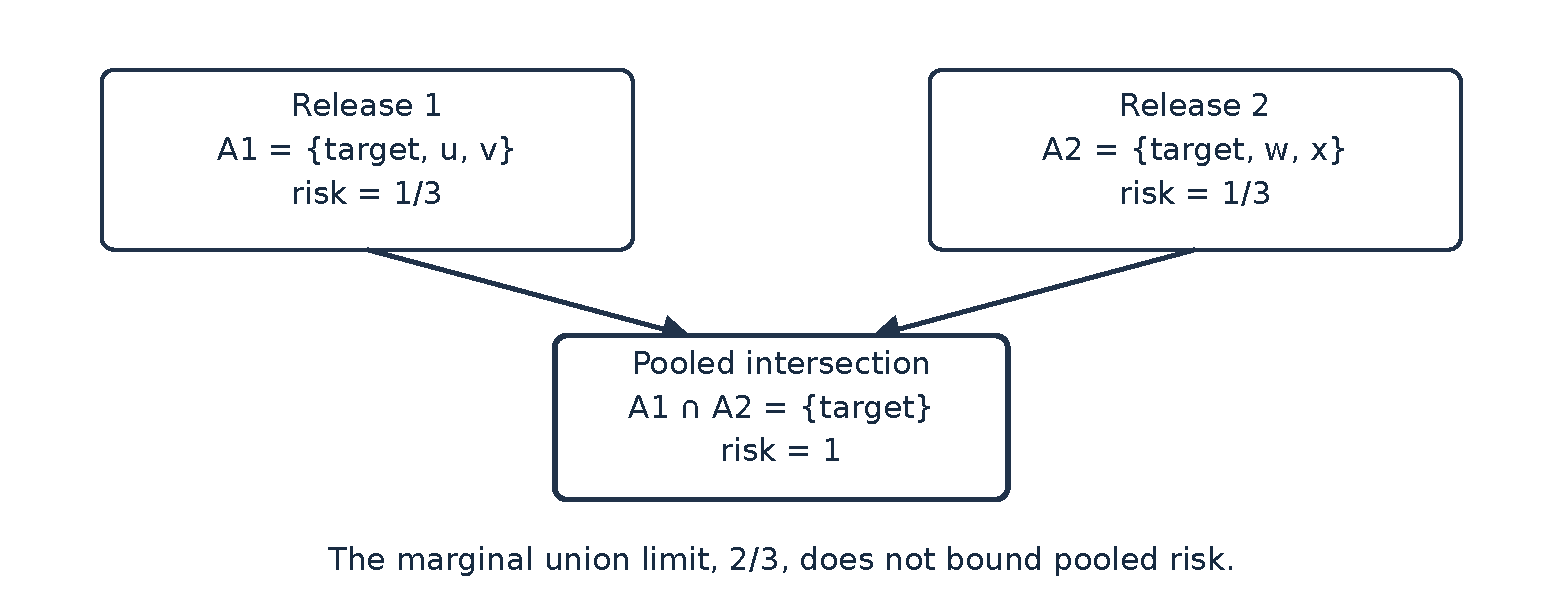
\includegraphics[width=.94\linewidth]{diagrams/pooling.pdf}
\caption{Pooling intersects candidate sets. This illustrative construction assumes uniform selection within each displayed set; it is distinct from the measured four-release simulation.}
\label{fig:pool-diagram}
\end{figure}


The larger difficulty is that $C_\cup$ is the wrong event. An adversary who holds
all $m$ releases is not restricted to using them one at a time. It applies a
joint linkage rule
\begin{equation}
\delta_a^{(m)} : \mathcal{Z} \times \mathcal{Y}_1 \times \cdots \times
\mathcal{Y}_m \longrightarrow I \cup \{\emptyset\} ,
\label{eq:joint}
\end{equation}
and the programme-level risk is $R_{\mathrm{pool}} = \Prob\{\delta_a^{(m)} =
t\}$, which is not contained in the union $C_\cup$.

\begin{proposition}[Marginal risks do not bound pooled risk]\label{prop:nopool}
Let $m \geq 2$. Suppose each released record carries a pseudonym that is the same
in every release, so that records can be matched across releases, and the adversary
knows the target's full quasi-identifier vector, from which it forms the target's key
in every release. For every $\nu > 0$ there exist a population, a sample and $m$
releases such that $R_i \leq \nu$ for every $i$ while
$R_{\mathrm{pool}} = 1$. Consequently no upper bound on $R_{\mathrm{pool}}$ can
be written as a function of $(R_1, \dots, R_m)$ alone. If each release
publishes the candidate set implied by its key and the adversary selects
uniformly from the intersection of those sets, then $R_{\mathrm{pool}}$ is
nondecreasing in $m$ and satisfies $R_{\mathrm{pool}} \geq \max_i R_i$.
\end{proposition}

\begin{proof}
See Appendix \ref{app:proofs}. The construction takes $n = k^m$ units labelled
by vectors in $\{1, \dots, k\}^m$ and lets release $i$ key on all coordinates
except the $i$th, so that every release is $k$-anonymous while the intersection
of the $m$ candidate sets is a singleton.
\end{proof}

Proposition \ref{prop:nopool} does not depend on the construction. Section
\ref{sec:composition} builds four releases from ordinary demographic keys, each
carrying a minimum cell count of three and containing no unique record at all,
and the pooled attack identifies the target with probability 0.4581 against a
Boole upper bound of 0.2530. Two releases are already enough: the pooled risk at
$m = 2$ is 0.4114, against a Boole bound of 0.148 for those two releases, and it is 1.6 times the bound of all four.

Neither the phenomenon nor its direction is new. \citet{ganta2008} showed that
independent releases of overlapping populations, each protected by a syntactic
rule, can be combined into a successful attack, and the failure of syntactic
criteria under composition is the standard argument for a formal accountant
\citep{dwork2006a,dwork2014}. \citet{cohen2020} prove the same failure for a
formal version of the legal notion of singling out: more than logarithmically
many exact counts, each safe alone, let an adversary single out a record. What Proposition \ref{prop:nopool} adds is a
statement in the terms institutions use to certify releases. The
composition-attack literature shows that combining releases can break a syntactic rule;
the proposition says that no function of the published marginal risks can bound
the combined risk, so the quantity a release programme is certified against is
not the quantity that governs it. Section \ref{sec:eval} then measures that gap on
a release system with an operational lever, which is the part of the argument the
earlier work does not supply.

Three consequences follow for practice. Marginal risk figures may be published,
but they license no programme-level claim. A programme tolerance must be
assessed by direct joint simulation under \eqref{eq:joint}, with shared targets
and shared auxiliary information; separate simulations of each release cannot
recover cross-release dependence by construction, because they never form the
intersection. And a formal accountant, discussed in Section \ref{sec:dp}, is
the one device that does compose without a dependence assumption.

\subsection{Allocating a programme tolerance}

Suppose an institution accepts the conservative route and governs the union
event, so that the programme constraint is $\sum_i R_i \leq \tau_{\mathrm{prog}}$
by \eqref{eq:boole}. Each release has value weight $w_i > 0$ and frontier
$\varphi$ shared across releases for simplicity.

\begin{proposition}[Risk budget]\label{prop:budget}
The problem $\max \sum_i w_i \varphi(r_i)$ subject to $\sum_i r_i \leq
\tau_{\mathrm{prog}}$ and $r_i \geq 0$, with $\varphi$ increasing,
differentiable and strictly concave, and with $\varphi'(0^+) = \infty$, so that no release is
allocated zero risk, has a unique solution characterised by
\begin{equation}
w_i \varphi'(r_i^\star) = \mu \quad \text{for all } i, \qquad
\sum_i r_i^\star = \tau_{\mathrm{prog}} ,
\label{eq:water}
\end{equation}
for a multiplier $\mu > 0$. If $\varphi(r) = \log r$ then $r_i^\star =
\tau_{\mathrm{prog}} w_i / \sum_j w_j$, so the budget is allocated in
proportion to value.
\end{proposition}

\begin{proof}
See Appendix \ref{app:proofs}.
\end{proof}

The equal split $r_i = \tau_{\mathrm{prog}}/m$, which is what an institution
does by default when it applies one tolerance to every release, satisfies
\eqref{eq:water} only if all $w_i$ are equal. The proportional rule is equally
particular: it holds for the logarithmic value curve and for no other. For the
power family $\varphi(r) = a + b r^{\gamma}$ with $b < 0$ and $\gamma < 0$,
which is the family that fits the simulated frontier, condition
\eqref{eq:water} gives
\begin{equation}
r_i^\star \ \propto \ w_i^{1/(1-\gamma)} ,
\label{eq:power}
\end{equation}
so the allocation is flatter than value whenever $\gamma < 0$, and it
approaches an equal split as $\gamma \to -\infty$. In the simulation the fitted $\gamma = -0.23$ gives an exponent of 0.81, and
the resulting allocation cuts the total loss by 4.5 per cent relative to the
equal split.

We stress the scope. Proposition \ref{prop:budget} governs the union event. It
does not govern the pooled attack, and by Proposition \ref{prop:nopool} nothing
stated in terms of the marginals can. A risk budget is a device for allocating
attention across releases, not a substitute for joint simulation.

\section{Adaptive attacks and anytime-valid certification}\label{sec:sequential}

The preceding analysis fixes the number of releases and attacks. An operational
adversary does neither: it observes a new vintage, decides whether to acquire more
auxiliary information, and stops when the posterior is sufficiently favourable.
An institution also monitors its simulation and may be tempted to stop when the
bound first passes. Fixed-sample intervals do not generally survive either form
of optional stopping. \citet{wald1945} built tests for data that arrive one
observation at a time, \citet{darling1967} and \citet{lai1976} gave confidence
sequences that hold at every sample size, and \citet{johari2022} show how
repeated looks at an online experiment inflate the error of a fixed-sample
test.

Let $\mathcal F_s=\sigma(Y_1,\ldots,Y_s,Z^{(s)})$ be the information available
after release $s$, including auxiliary information acquired adaptively, and let
$H_t$ be the hypothesis that candidate record $j$ belongs to target $t$. The
posterior odds process is
\begin{equation}
O_s(H_t)=O_0(H_t)\prod_{v=1}^s
\frac{p(Y_v,Z^{(v)}\mid H_t,\mathcal F_{v-1})}
     {p(Y_v,Z^{(v)}\mid H_t^c,\mathcal F_{v-1})}.
\label{eq:sequential-odds}
\end{equation}
The conditional densities in \eqref{eq:sequential-odds} prevent the common error
of multiplying marginal likelihoods from dependent vintages. Revisions, common
records and mechanism randomness shared across releases must remain in the
conditioning history.

An adversary need not use the arbitrary posterior threshold one half. Suppose a
correct allegation produces benefit $h>0$, a false allegation costs $c_f\ge0$,
and making the allegation costs $c_a\ge0$. At posterior match probability $p$,
the expected payoff is $ph-(1-p)c_f-c_a$.

\begin{proposition}[Economically rational attack threshold]
\label{prop:attack-threshold}
An expected-payoff-maximising adversary acts if and only if
\begin{equation}
p\ge p^\star:=\min\left\{1,\frac{c_f+c_a}{h+c_f}\right\}.
\label{eq:attack-threshold}
\end{equation}
The threshold equals one half only in the special case $h=c_f$ and $c_a=0$.
\end{proposition}

The attack evaluation must therefore report the precision--coverage curve over
$p^\star$, or state the payoff assumptions that select one point. A low average
success rate can coexist with a high-payoff attack that makes few, accurate
allegations.

For institutional monitoring, let $X_b\in\{0,1\}$ be success in simulated attack
$b$, $S_B=\sum_{b\le B}X_b$, and consider a candidate risk $r\in(0,1)$. Mixing
the Bernoulli likelihood ratio against a $\mathrm{Beta}(a,b)$ alternative gives
the e-process
\begin{equation}
E_B(r)=
\frac{\mathrm B(a+S_B,b+B-S_B)}{\mathrm B(a,b)
r^{S_B}(1-r)^{B-S_B}}.
\label{eq:eprocess}
\end{equation}

\begin{proposition}[Anytime-valid risk sequence]\label{prop:anytime}
If the simulated attacks are conditionally Bernoulli with risk $r_0$, then
$\{E_B(r_0),\mathcal F_B\}_{B\ge0}$ is a nonnegative martingale with initial
value one. Consequently
\begin{equation}
\Prob_{r_0}\!\left\{\sup_{B\ge1}E_B(r_0)\ge\alpha^{-1}\right\}\le\alpha.
\label{eq:ville}
\end{equation}
The confidence sequence
\begin{equation}
\mathcal C_B=\{r\in(0,1):E_B(r)<\alpha^{-1}\}
\label{eq:cs}
\end{equation}
therefore contains $r_0$ simultaneously for every monitoring time with
probability at least $1-\alpha$ \citep{ville1939,howard2020,howard2021}. The
betting construction of \citet{waudbysmith2024} gives narrower sequences for
bounded means, and \eqref{eq:eprocess} is an instance of the e-values studied
by \citet{vovk2021} and \citet{grunwald2024}.
\end{proposition}

For a family of $q$ targets, mechanisms or subgroups fixed before any outcome
is seen, replace $\alpha$ by $\alpha/q$ in \eqref{eq:cs}; the union bound then
gives simultaneous anytime coverage without independence. The correction is not
valid when $q$ or the choice of family depends on the outcomes. If hypotheses
are added after inspection, $\alpha$ must be allocated by a spending sequence
registered in advance \citep{foster2008,tian2021}, which is the construction of the
companion article. A
hierarchical or max-e-process can recover power only if its dependence model is
declared before the results are observed. Control of the false discovery rate
\citep{benjamini1995} is a weaker guarantee and does not suit a certificate,
which must hold for every release it covers.

Finally, calibration on one attack distribution $P$ does not transport without
a condition on the deployment distribution $Q$. For the success indicator
$0\le C\le1$,
\begin{equation}
R_Q-R_P=\E_Q C-\E_P C\le \|Q-P\|_{\mathrm{TV}}
\le\sqrt{\frac12D_{\mathrm{KL}}(Q\|P)},
\label{eq:shift}
\end{equation}
where the second inequality is Pinsker's inequality. Thus a declared
KL-neighbourhood $D_{\mathrm{KL}}(Q\|P)\le\rho$ gives the transport bound
$R_Q\le\min\{1,R_P+\sqrt{\rho/2}\}$. This is not a claim that KL balls describe
every future adversary. It is a computable sensitivity statement, and the pipeline
implements \eqref{eq:eprocess}--\eqref{eq:shift}, so optional stopping and
distribution shift are measured here rather than listed as verbal limitations.

\subsection{What the pipeline measures}\label{sec:sequential-evidence}

The three devices above are implemented in the packaged pipeline, and this
subsection reports what they give on the release system of Section
\ref{sec:eval}. The reference attack throughout is the pooled one against the
$5$-anonymous release, whose success rate is 0.224.

\paragraph{Monitoring is not free, and pretending otherwise is worse.}
Take an institution that simulates 4{,}000 attacks and looks at its
bound 20 times along the way. The study records whether the bound falls below
the true risk at any of the 20 looks, which is the event that an institution
free to stop at any look could release on a bound that is wrong. Over 500 such
runs the fixed-sample bound at the 5 per cent level falls below the true risk at
some look in 20 per cent of them. The confidence sequence
\eqref{eq:cs} does so in 0 per cent. The stated level of a
fixed-sample interval is a statement about one prearranged sample size, and an
institution that watches its own simulation is not making that statement.

The inferential cost of optional stopping is a wider interval, and it is small. On the same
counts the fixed-sample upper bound is 0.235 and the anytime bound is
0.249, a ratio of 1.06 over the runs of the study.

\begin{table}[t]
\centering
\caption{The cost of watching the run. The fixed-sample column is the number of successless attacks that certifies the tolerance at one prearranged sample size. The anytime column is the number that certifies it while the institution monitors and may stop whenever it likes, using the confidence sequence of Proposition \ref{prop:anytime} with a uniform prior. The last column is the ratio. It is the price of that mixture, which stays able to certify after a success is seen, and not of monitoring itself: a predeclared point alternative at zero risk is also anytime-valid and certifies after the fixed-sample count, but can never certify once a success occurs.}
\label{tab:anytime}
\begin{tabular}{rrrrr}
\toprule
Tolerance $\tau$ & $\alpha$ & Fixed sample & Anytime & Ratio \\
\midrule
0.01 & 0.05 & 299 & 984 & 3.3 \\
0.001 & 0.05 & 2{,}995 & 12{,}417 & 4.1 \\
\bottomrule
\end{tabular}
\end{table}


Table \ref{tab:anytime} gives the certification counts of Proposition
\ref{prop:cert} beside those of the confidence sequence. With the uniform
mixture used here, anytime certification of a tolerance of $10^{-3}$ at the 5
per cent level needs 12{,}417 successless attacks, against 2{,}995 at a sample
size fixed in advance. A predeclared point alternative at zero risk gives an
anytime-valid test that certifies after 2{,}995, the fixed-sample count, but it
can never certify once a success is seen. The larger figure is therefore the
price of staying able to certify after successes, not of monitoring itself, and
the ratio column of Table \ref{tab:anytime} should be read in that sense.

\paragraph{The adversary's threshold is a payoff, not a convention.}
Table \ref{tab:adversary} reads the same attack at the thresholds three payoff
structures imply. An adversary that gains and loses equally and pays nothing to
allege acts at one half, and collects a yield of 0.084 successful
allegations per target. An adversary that gains ten times what a false allegation
costs it acts at 0.136 instead: it acts on 0.355 of
targets, is right 0.463 of the time, and its yield is
0.165, more than double the first. An adversary facing reputational or
legal cost for a false allegation acts at 0.917, on
0.034 of targets, and is right 0.978 of the
time.

\begin{table}[t]
\centering
\caption{Where a paid adversary acts. The payoff of a correct allegation, the cost of a false one and the cost of making any allegation fix the posterior threshold of Proposition \ref{prop:attack-threshold}. Coverage is the share of targets the adversary acts on at that threshold, precision the share of those allegations that are true, and yield the product, which is what the adversary collects. The attack is the pooled one against k anonymity 5. One half, the threshold usually assumed, is the middle case of equal stakes and free allegations.}
\label{tab:adversary}
\begin{tabular}{rrrrrrr}
\toprule
Benefit $h$ & False cost $c_f$ & Action cost $c_a$ & $p^\star$ & Coverage & Precision & Yield \\
\midrule
1 & 1 & 0 & 0.500 & 0.179 & 0.814 & 0.146 \\
10 & 1 & 0.5 & 0.136 & 0.395 & 0.556 & 0.220 \\
1 & 5 & 0.5 & 0.917 & 0.083 & 0.994 & 0.082 \\
\bottomrule
\end{tabular}
\end{table}


The three rows are the same attack on the same release. An evaluation that reports
one threshold reports one row of a curve the adversary chooses from, and an
institution that assumes one half is assuming a payoff structure it has not stated.
The precision--coverage curve belongs in the release record with the risk estimate.

\paragraph{Distribution shift requires an explicit risk allowance.}
The transport bound \eqref{eq:shift} turns a declared neighbourhood into a number.
At a divergence of 0.05 the risk of the reference attack is
bounded by 0.382, against 0.274 at the smallest
neighbourhood in the table. Read the other way, and this is the more useful
direction, the bound says how much shift a release can absorb before it breaks its
tolerance. The reference release can absorb none: its pooled risk already exceeds
the tolerance of 0.12, so any neighbourhood at all leaves it inadmissible. Of the
releases that meet the tolerance pooled, noisy counts at $\varepsilon=1$, with a
pooled risk of 0.004 over six vintages, can absorb a divergence of 0.027 and no
more. That is a small neighbourhood, and
saying so is an honest statement of how much the certificate depends on the
adversary specification, which the usual sensitivity paragraph leaves
unquantified.


\section{Formal privacy is a different regime}\label{sec:dp}

A randomised mechanism $M$ is $(\varepsilon, \delta_{\mathrm{dp}})$-differentially
private if, for all neighbouring datasets $x \sim x'$ and all measurable output
sets $E$,
\begin{equation}
\Prob\{M(x) \in E\} \leq e^{\varepsilon}\,\Prob\{M(x') \in E\}
+ \delta_{\mathrm{dp}} .
\label{eq:dp}
\end{equation}
For mechanisms $M_i$ with parameters $(\varepsilon_i, \delta_{\mathrm{dp},i})$,
basic adaptive composition gives $\varepsilon_{\mathrm{tot}} = \sum_i
\varepsilon_i$ and $\delta_{\mathrm{dp,tot}} = \sum_i \delta_{\mathrm{dp},i}$, and tighter accountants are
available \citep{dwork2010,kairouz2017,bun2016,mironov2017,dong2022}. Even the basic form shows the
structural difference from Section \ref{sec:comp}: the composition holds without
any assumption about the adversary or about dependence between releases.

The parameter $\varepsilon$ bounds the change in output distributions for
neighbouring databases. It is not the probability that an identified person is
correctly linked, and the two must not be compared on a common numerical scale.
The relation that does hold is Bayesian and depends on the prior.

\begin{proposition}[What $\varepsilon$ permits]\label{prop:dpbound}
Let $M$ satisfy \eqref{eq:dp} with $\delta_{\mathrm{dp}} = 0$, and let $H$ be a
hypothesis about a single individual such that the databases $x$ and $x'$ under
$H$ and its negation differ only in that individual's record, the rest of the
database having the same distribution under both.
For a Bayesian adversary with prior $\Prob(H) = p$, the posterior after
observing that the release falls in a measurable set $E$ of positive
probability satisfies
\begin{equation}
\Prob(H \mid M \in E) \ \leq \
\frac{e^{\varepsilon} p}{e^{\varepsilon} p + (1 - p)} .
\label{eq:dppost}
\end{equation}
\end{proposition}

\begin{proof}
See Appendix \ref{app:proofs}; the argument is the Bayesian reading of
differential privacy in \citet{kasiviswanathan2014}.
\end{proof}

Inequality \eqref{eq:dppost} is the honest translation, and it shows why no
single number does both jobs. With a prior of $0.1$, which is what a 10-anonymous
key class supplies under exact exchangeable matching, $\varepsilon = 0.5$
permits a posterior of 0.155, $\varepsilon = 1$ permits 0.232 and
$\varepsilon = 2$ permits 0.451. With a prior of $1/3$ the same
$\varepsilon = 1$ permits 0.576. An institution that adopts $\varepsilon = 1$
has not chosen a tolerance of 1; it has chosen a multiplier on whatever prior
the adversary brings, and the tolerance it has implicitly accepted depends on
the key structure of the file.

The two regimes therefore answer different questions and both belong in the
record. Scenario-conditional risk answers what a named adversary would achieve
against this release, which is the question a governance committee, a data
protection authority and an affected person all ask. Formal privacy bounds how far
any adversary's odds about one record can move relative to that record's
absence, under independence of records, and it composes across a programme,
which scenario analysis cannot do because Proposition \ref{prop:nopool} denies
it a composition theorem. \citet{kifer2011} shows that
neither can be made assumption-free, and the Pufferfish framework of
\citet{kifer2014} makes the adversary's prior an explicit input, which is the
formal counterpart of a declared scenario. \citet{kairouz2017} and
\citet{balle2020} read the guarantee as a limit on the power of any test between
neighbouring datasets, in the sense of \citet{neyman1933}. The practical arrangement is to run a
formal accountant for the programme budget and a scenario assessment for the
release decision, and to report them separately with their assumptions attached.

The distinction is worth stating in one line, because it decides which tool an
institution should reach for. The framework of this paper is
adversary-specific: it answers what happens if someone with these resources
attacks this release, and the answer is a probability that can be compared with a
tolerance and audited against a stated attacker. Differential privacy is
adversary-agnostic: it answers how much any observer's beliefs can move because
one person's record was included, whoever that observer is and whatever it knows,
and the answer is not a linkage probability. The first is what a release committee
needs, because a committee must justify a decision about a particular publication
to a particular public. The second is what a programme needs, because it is the
only device that composes without an assumption about how releases relate to one
another. An institution that wants both should hold both, and should not attempt
to convert one number into the other.

\section{Simulation study}\label{sec:sim}

The results above are statements about any release. This section applies them
to a synthetic register where the population is known, so that every estimate
can be compared with a truth. All quantities come from one program with
fixed seeds; Appendix \ref{app:sim} gives the details.

\subsection{Design}

The population has $N = 200{,}000$ units. Each unit carries a district (40
categories with a skewed size distribution), sex, age in single years from 18
to 87, and an occupation group (12 categories, also skewed). The adversary's
key is the cross-classification of district, sex, five-year age band and
occupation group, giving 13,440 possible cells of which 12,596 are occupied.
1,305 cells are population unique, so 0.65 per cent of the population would be
identifiable from the key alone in a census.

The confidential variable is
\begin{equation}
y_i = 8 + \psi_{d(i)} + \omega_{o(i)} + 0.018\,(\mathrm{age}_i - 50)
+ 0.10\,\mathrm{sex}_i + \epsilon_i , \qquad
\epsilon_i \sim N(0, 0.6^2) ,
\end{equation}
with district and occupation effects drawn once from $N(0, 0.45^2)$ and
$N(0, 0.35^2)$. A Bernoulli sample with $\pi = 0.05$ gives $n = 10{,}035$
records containing 4,679 distinct keys, of which 2,729 are unique, so 27.2 per
cent of the released records are sample unique.

The release supports three declared analyses: the mean of $y$ by district, by
five-year age band, and by occupation. Utility \eqref{eq:util} is the negative
of the average of the three root mean squared errors, each computed at the
finest classification its analysis needs and normalised by the standard
deviation of $y$, plus a penalty of $0.5$ times the share of target categories
the release leaves unreportable. Coarsening the key therefore costs accuracy on the analysis it coarsens, and
suppression costs coverage, so both levers reduce measured utility. The two interact: once
a minimum cell count binds, coarsening also buys back records, so the levers are
substitutes as well as costs, which is why the frontier has to be traced rather
than reasoned out.

The declared adversary observes district and sex without error, the released
age band with probability 0.15 of a one-band error, the occupation group with
probability 0.10 of a wrong group, and a noisy reading $z_t = y_t + N(0,
0.75^2)$ of the confidential variable. It links by maximum posterior under the
same error model that generates the error, which is \eqref{eq:post} with a flat
prior over the records in the target's district and sex. The uncertainty set
$H_a$ in \eqref{eq:rob} contains two adversaries, the declared one and one
whose covariate is twice as precise, each modelling its own information
correctly. The robust risk is the larger, and across all 45 settings of the
grid it is attained by the more capable adversary, whose risk runs from 1 to 76
per cent above the declared one, with a median gap of 40 per cent.

Two target sets are reported, because as Section \ref{sec:gov} insists they are
different controls. The first is a target drawn uniformly from the released
records, whose risk is an average; this is the coordinate used for the frontier
and the mechanism grid. The second is the set of records sitting in the smallest
released cells, whose risk is estimated target by target and summarised by its
maximum; this is the supremum control of \eqref{eq:admiss} and it is the
stricter of the two.

The mechanism family is a grid of 45 settings: age band width in
$\{5, 10, 20\}$ years, occupation groups in $\{12, 6, 3\}$, and minimum cell
count $k_{\min} \in \{1, 3, 5, 10, 20\}$ with records in smaller cells
suppressed. A district record swapping lever \citep{fienbergmcintyre2004} was
built and then removed, for a
reason that belongs in the paper rather than a footnote. Swapping reduced the simulated risk, but only against an
adversary that takes the released district at face value, and the declared
scenario gives no reason to assume that. Its apparent protection was a property
of the assumed adversary rather than of the release, which is the failure that
Section \ref{sec:est} warns about, and the honest response was to drop the lever
rather than to report a risk figure that depends on it.

\subsection{The conventional measures disagree by orders of magnitude}

Table \ref{tab:measures} reports the standard summaries for the unprotected
release. The identity \eqref{eq:marksamp} holds exactly: the mean
sample-frequency risk and $D_I/n$ are the same number, 0.4663. The
population-frequency version is 0.0636, and the unconditional measure
\eqref{eq:markpop}, which carries the inclusion probability of
\eqref{eq:factor}, is 0.0233. The sample-frequency measure is 7.3 times the
population-frequency version and 20 times the unconditional one, and all three
have been published under the same label.

\begin{table}[t]
\centering
\caption{Conventional risk summaries for the unprotected release ($N = 200{,}000$, $\pi = 0.05$, $n = 10{,}035$).}
\label{tab:measures}
\begin{tabular}{llr}
\toprule
Measure & Experiment described & Value \\
\midrule
Prosecutor, mean $1/f_k$ & uniform choice among released candidates & 0.4663 \\
Prosecutor, $\max 1/f_k$ & worst released record & 1.0000 \\
Share of records with $f_k = 1$ & sample uniqueness & 0.2719 \\
Marketer, $D_I/n$ & identity \eqref{eq:marksamp}, same experiment & 0.4663 \\
Plug-in $n^{-1}\sum_i 1/F_{K(i)}$ & population frequencies assumed known & 0.0636 \\
Marketer, unconditional \eqref{eq:markpop} & membership unknown, $\pi$ applied & 0.0233 \\
$\pi$ times the plug-in measure & neither experiment; reported anyway & 0.0032 \\
Uniqueness probability $\rho$, truth & $\Prob(F_k = 1 \mid f_k = 1)$, computed & 0.0227 \\
Uniqueness probability $\rho$, model-based & fitted negative binomial for $F_k$ & 0.0274 \\
Journalist, naive $\pi$ & sampling fraction used as the risk & 0.0500 \\
\bottomrule
\end{tabular}
\end{table}


The journalist row deserves attention because it is the one measure that needs
a model for an unobservable. Since binomial thinning of a negative binomial law
is negative binomial with the same dispersion, the population frequency law is
identified from the sample cell counts, and the fit recovers a mean population
cell size of 14.83 against a truth of 14.88, within 1 per cent. Figure
\ref{fig:journ} compares the resulting $\rho$ with the truth across sampling
fractions. The model-based estimate is conservative at every sampling
fraction and its relative error lies between 8 and 25 per cent. Using $\pi$ itself as
the risk, which is a common shortcut, overstates the truth at every sampling
fraction, by a factor of 2.20 at $\pi = 0.05$ and 1.64 at $\pi = 0.5$.

\begin{figure}[t]
\centering
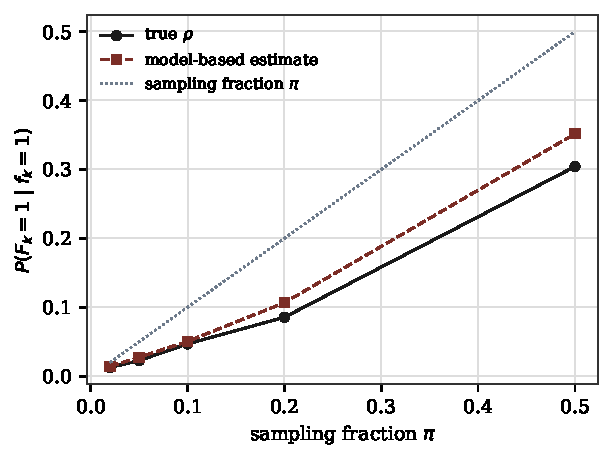
\includegraphics[width=0.62\textwidth]{figures/fig5_journalist.pdf}
\caption{Journalist risk $\Prob(F_k = 1 \mid f_k = 1)$ against the sampling
fraction. The model-based estimate uses a negative binomial population
frequency law fitted to the sample cell counts. The sampling fraction itself is
not an approximation to the risk.}
\label{fig:journ}
\end{figure}

\subsection{Measurement error does not simply reduce risk}

Under exact exchangeable matching the predicted success rate for a uniformly
drawn released target is 0.4663. Simulating the declared adversary with key
reporting error but no covariate gives 0.3812 over 5,000 replicates, which is
the reduction practitioners expect. Adding the single noisy covariate returns
the success rate to 0.4642 over 20,000 replicates, with a one-sided 95 per cent
bound of 0.4701. The reciprocal-frequency figure is therefore accurate for this
release, but by cancellation between an error that spreads posterior mass and a
covariate that concentrates it. An assessment that modelled only the reporting
error would have understated the risk by 18 per cent.

Figure \ref{fig:calib} tests the posterior itself, which is the first
falsification requirement of Section \ref{sec:falsify}. When the adversary's
declared model matches the process that generates its information, the mean gap
between the binned maximum posterior and the empirical success rate is 0.007.
When the adversary assumes a covariate 2.5 times noisier than the truth, the mean gap rises to 0.049 and the miscalibration is one-sided: the posterior
understates the success rate in the lower bins. The overall success rate barely
moves, from 0.4642 to 0.4571. This is the practical lesson of the figure.
A single risk number cannot reveal that the linkage model is wrong, and a
calibration check on held-out matches can.

\begin{figure}[t]
\centering
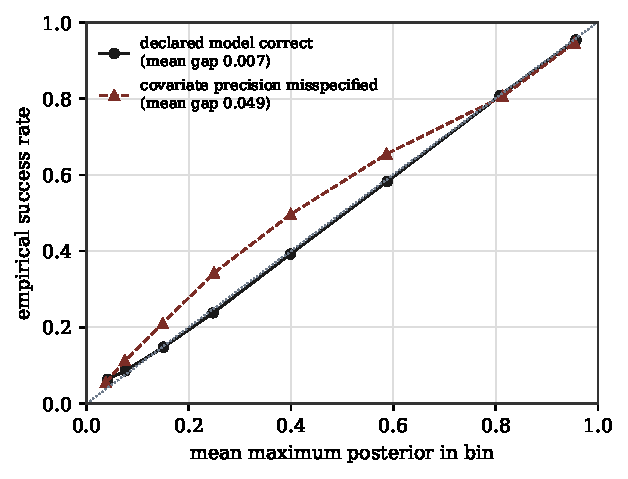
\includegraphics[width=0.58\textwidth]{figures/fig3_calibration.pdf}
\caption{Calibration of the adversary's maximum posterior against the empirical
success rate, 20,000 replicates per curve. The two models produce risk estimates
that differ by 0.007, while their calibration gaps differ by a factor of seven.}
\label{fig:calib}
\end{figure}

\subsection{$k$-anonymity does not deliver $1/k$}\label{sec:kanon}

Table \ref{tab:kanon} applies minimum cell counts and compares the nominal
bound $1/k$ with two simulated quantities: the average risk over a uniformly
drawn released target, and the risk of the worst target among those in the
smallest released cells, each of the latter estimated from 250 replicates.

The average risk stays below $1/k$ at $k = 3$ and $k = 5$ and exceeds it at
$k = 10$ and $k = 20$. The worst target's risk exceeds $1/k$ at every $k$, and so does its one-sided
95 per cent lower confidence bound, which is 0.82, 0.78, 0.64 and 0.68 as $k$
runs from 3 to 20. Those bounds carry a Bonferroni correction for the number of
targets examined, since the worst target is selected on its own estimate.
Between 27 and 75 per cent of the targets in minimum-size cells have an
individual lower bound above $1/k$. Both comparisons
refute the reading of $k$-anonymity as a guarantee that no released person faces
a risk above $1/k$, and the second refutes it in the form that matters for rule
\eqref{eq:admiss}, which is stated as a supremum. The mechanism is the one
Proposition \ref{prop:kanon} names: the covariate separates members of a key
class, and raising $k$ shrinks the share of the adversary's information that the
criterion controls while leaving the covariate untouched.

Figure \ref{fig:riskdist} shows what the suppression does to the whole risk
distribution rather than to its maximum, and the utility loss is large. Reaching
$k = 10$ retains 15.5 per cent of the released records and reaching $k = 20$
retains 4.8 per cent, so a release governed by its maximum prosecutor risk
alone is pushed towards discarding most of its own content.

\begin{table}[t]
\centering
\caption{Minimum cell counts against the simulated risk of the declared adversary. The average uses 12{,}000 uniformly drawn targets with $\overline{R}_{0.95}$ its one-sided Clopper--Pearson bound. The worst target is taken over the listed number of targets in minimum-size cells, each estimated from 250 replicates, and is reported with a one-sided 95 per cent lower bound carrying a Bonferroni correction for the number of targets examined. The last column is the share of those targets whose individual lower bound exceeds $1/k$.}
\label{tab:kanon}
\small
\begin{tabular}{rrrrrrrrr}
\toprule
$k_{\min}$ & Kept & Share & $1/k$ & Average & $\overline{R}_{0.95}$ &
Targets & Worst (bound) & Share above $1/k$ \\
\midrule
3 & 5{,}426 & 0.541 & 0.3333 & 0.2573 & 0.2640 & 250 & 0.900 (0.817) & 0.748 \\
5 & 3{,}361 & 0.335 & 0.2000 & 0.1852 & 0.1911 & 250 & 0.868 (0.778) & 0.492 \\
10 & 1{,}555 & 0.155 & 0.1000 & 0.1129 & 0.1178 & 230 & 0.744 (0.638) & 0.326 \\
20 & 484 & 0.048 & 0.0500 & 0.0787 & 0.0828 & 60 & 0.768 (0.675) & 0.267 \\
\bottomrule
\end{tabular}
\end{table}


\begin{figure}[t]
\centering
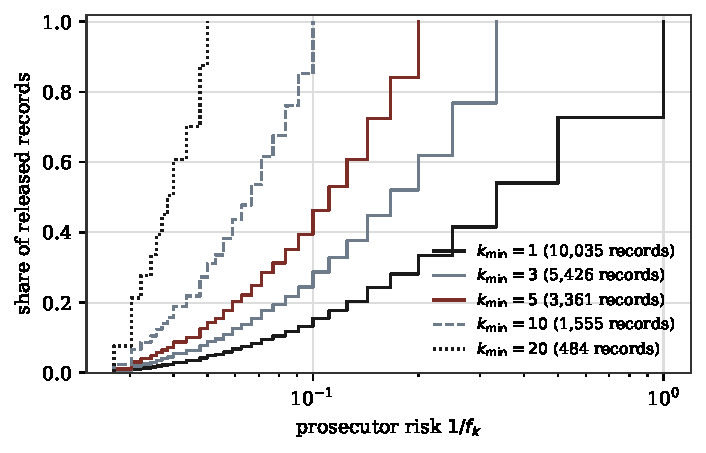
\includegraphics[width=0.66\textwidth]{figures/fig1_risk_distribution.pdf}
\caption{Distribution of prosecutor risk $1/f_k$ across released records under
minimum cell counts. Governing the maximum alone forces most of the file out of
the release.}
\label{fig:riskdist}
\end{figure}

\subsection{Frontier, tolerance and the relative weight assigned to harm}

Figure \ref{fig:frontier} plots all 45 mechanism settings in the plane of the
one-sided risk bound and the utility of Section \ref{sec:ru}. Eleven settings
are nondominated, and the frontier spans risk from 0.081 to 0.564. It is steep
at the low-risk end: halving the bound from 0.1715 to 0.0806 costs 0.17 of
utility, half the range the frontier spans, and cuts the records retained from
100 to 58 per cent.

The attainable frontier is not concave. Successive slopes of the eleven
nondominated points run from 6.0 down to 0.006 and not monotonically,
which is what a discrete mechanism family produces and what Proposition
\ref{prop:exist} anticipates. A three-parameter power curve fits it with $R^2 = 0.964$ and is concave over the
fitted range; it is used only for the allocation
in Section \ref{sec:composition}. Table \ref{tab:tau} reports the implied
tolerance of Proposition \ref{prop:tau}, computed as the value-maximising choice
over the eleven nondominated settings rather than on the fitted curve, and with
the one-sided bound as the risk coordinate as \eqref{eq:admiss} requires.

Two features matter for practice. The implied tolerance is flat over wide
ranges, since one setting is optimal from $\kappa = 5$ to $\kappa = 10$, and it
jumps between ranges: doubling the relative weight assigned to harm from $\kappa = 0.5$ to $\kappa = 1$ cuts the tolerance
from 0.345 to 0.145 and moves the release from an unsuppressed file with twelve
occupation groups to one with three groups and a minimum cell count of five. The jump is a property of the discrete mechanism
family, not of the argument, and it has a practical reading: over most of the
range an institution cannot fine-tune its tolerance, and near a breakpoint a
small revision of the relative weight assigned to harm changes the release.

\begin{figure}[t]
\centering
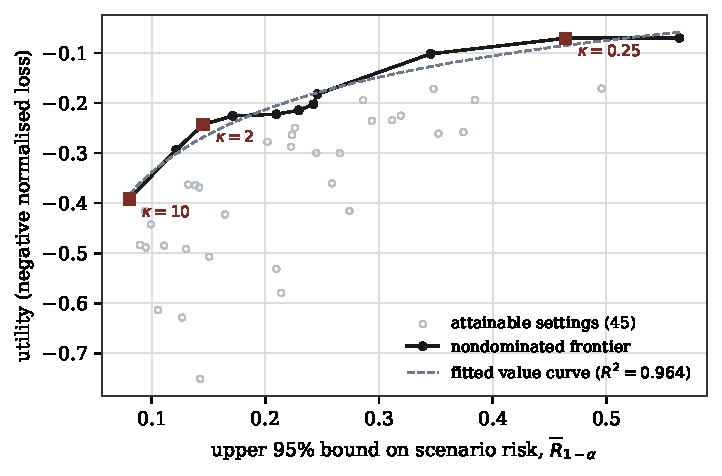
\includegraphics[width=0.72\textwidth]{figures/fig2_frontier.pdf}
\caption{Risk--utility plane for 45 mechanism settings. The risk coordinate is
the one-sided 95 per cent bound for a uniformly drawn target, not the point
estimate. Squares mark the value-maximising setting for three values of the
relative harm weight $\kappa$; the associated risk is the implied
tolerance $\tau^\star$ of Proposition \ref{prop:tau}.}
\label{fig:frontier}
\end{figure}

\begin{table}[t]
\centering
\caption{Tolerance implied by the relative harm weight, computed by maximising $U - \kappa \overline{R}_{0.95}$ over the nondominated settings. The selected setting reports age band width in years, occupation groups and minimum cell count.}
\label{tab:tau}
\begin{tabular}{rrlr}
\toprule
$\kappa = c_h/\lambda$ & Implied $\tau^\star$ & Selected setting & Records kept \\
\midrule
0.25 & 0.464 & 10-year bands, 12 groups, $k_{\min} = 1$ & 1.00 \\
0.50 & 0.345 & 20-year bands, 12 groups, $k_{\min} = 1$ & 1.00 \\
1.00 & 0.145 & 20-year bands, 3 groups, $k_{\min} = 5$ & 0.94 \\
2.00 & 0.145 & 20-year bands, 3 groups, $k_{\min} = 5$ & 0.94 \\
5.00 & 0.081 & 20-year bands, 3 groups, $k_{\min} = 20$ & 0.58 \\
10.00 & 0.081 & 20-year bands, 3 groups, $k_{\min} = 20$ & 0.58 \\
\bottomrule
\end{tabular}
\end{table}


\subsection{A programme of four releases}\label{sec:composition}

Four releases are built from the same sample. Release A keys on district, sex
and five-year age band; release B on district, sex and occupation; release C on
district, ten-year age band and six occupation groups; release D on sex,
ten-year age band and occupation. Each applies a minimum cell count of three,
so each is 3-anonymous and, by construction, no release contains a single
unique record. Their marginal risks, computed unconditionally so that a target suppressed from
a release contributes zero, are 0.0768, 0.0711, 0.0884 and 0.0168.

Table \ref{tab:comp} and Figure \ref{fig:comp} report what the programme
permits. The bounds implied by the marginals are $[0.0884, 0.2530]$ and the
independence value is 0.2313. An adversary that intersects the candidate sets of
the first two releases succeeds with probability 0.4114, which is 2.8 times the
bound of 0.148 implied by those two marginals and 1.6 times the upper bound implied
by all four. With all four releases the pooled risk
is 0.4581, which is 1.8 times that bound, and 26.0 per cent of targets are
uniquely identified by the intersection although none was unique in any single
release.

\begingroup\small\setlength{\tabcolsep}{3pt}\begin{table}[t]
\centering
\caption{Four 3-anonymous releases from one sample, 20{,}000 target replicates. No single release contains a unique record. Marginal risks are unconditional; a target suppressed from a release contributes zero to that release and does not narrow the intersection. The pooled adversary intersects the candidate sets of releases 1 to $m$ and selects uniformly from the intersection.}
\label{tab:comp}
\begin{tabular}{lrrr}
\toprule
& Records released & Marginal risk & Unique share \\
\midrule
Release A (district, sex, fine age) & 9{,}648 & 0.0768 & 0.000 \\
Release B (district, sex, occupation) & 9{,}709 & 0.0711 & 0.000 \\
Release C (district, ten-year age, six groups) & 9{,}257 & 0.0884 & 0.000 \\
Release D (sex, ten-year age, occupation) & 10{,}035 & 0.0168 & 0.000 \\
\midrule
\multicolumn{4}{l}{\emph{Programme-level quantities}} \\
Lower bound $\max_i R_i$ & & 0.0884 & \\
Upper bound $\min(1, \sum_i R_i)$ & & 0.2530 & \\
Value under independence & & 0.2313 & \\
Pooled attack, $m = 2$ & & 0.4114 & 0.208 \\
Pooled attack, $m = 3$ & & 0.4279 & 0.222 \\
Pooled attack, $m = 4$ & & 0.4581 & 0.260 \\
\bottomrule
\end{tabular}
\end{table}
\endgroup

\begin{figure}[t]
\centering
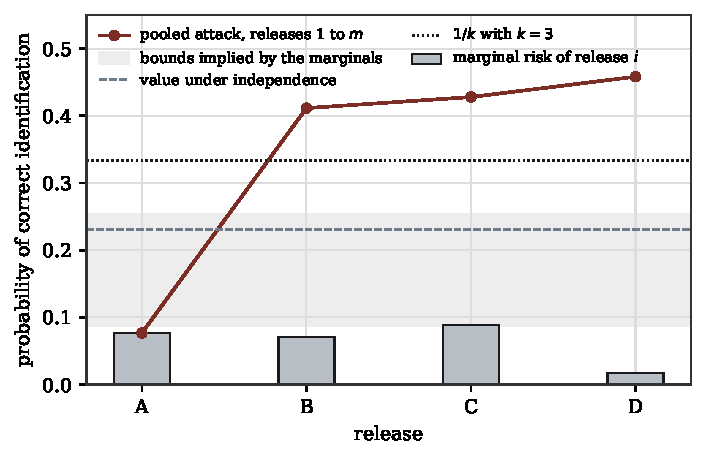
\includegraphics[width=0.72\textwidth]{figures/fig4_composition.pdf}
\caption{Marginal risks of four 3-anonymous releases and the risk of an
adversary that pools them. The shaded band is the interval implied by the
marginals under Proposition \ref{prop:boole}. The pooled attack leaves the band
at $m = 2$.}
\label{fig:comp}
\end{figure}

Two remarks. First, the effect is not driven by a large number of releases. Two
are enough, and the third and fourth add little because the first two already
carry most of the separating information. Second, ranking releases by their own
risk figures does not rank their contribution to the programme. Release D has the smallest marginal risk, 0.0168, yet adding it to the pool
raises the risk by 0.030, while release C, whose marginal risk is the largest at
0.0884, adds 0.017.
Both observations follow from Proposition \ref{prop:nopool} and neither is
visible in a marginal assessment.

Applying Proposition \ref{prop:budget} to the union event, with value weights
$1, 0.7, 0.5, 0.3$ and $\tau_{\mathrm{prog}} = 0.50$, the optimal allocation is
$(0.186, 0.139, 0.106, 0.070)$ against the equal split of $0.125$ each, and cuts
the total loss by 4.5 per cent. A constrained numerical optimum agrees with the
closed form \eqref{eq:power} to five decimal places, which is one check on both.
With the fitted $\gamma = -0.23$ the exponent in \eqref{eq:power} is 0.81, so the
allocation is flatter than the value weights. This is a real gain and a small
one, and it is available only for the union event.

\subsection{Does the gap survive at other register sizes?}\label{sec:scaling}

A synthetic study invites the question whether its findings are an artefact of
the size chosen. National registers hold millions of records, not the
200{,}000 of the main study. Table \ref{tab:scaling} rebuilds the same four
releases, with the same keys and the same minimum cell count, on registers of
4 sizes with the sampling fraction held fixed.

\begin{table}[t]
\centering
\caption{Does the pooling gap survive at other register sizes? The same four releases, the same keys and the same minimum cell count, rebuilt on registers of four sizes with the sampling fraction held fixed. Larger registers are safer release by release, because the key classes grow. The pooled attack falls more slowly, so the ratio of the pooled risk to the bound the marginals imply rises with size rather than falling. The gap the paper is about is not an artefact of the size chosen for the main study.}
\label{tab:scaling}
\small
\begin{tabular}{rrrrrrr}
\toprule
Population & Sample & Largest marginal & Pooled, 2 releases & Pooled, 4 & Boole bound & Ratio \\
\midrule
50{,}000 & 2{,}362 & 0.113 & 0.454 & 0.623 & 0.398 & 1.57 \\
100{,}000 & 5{,}056 & 0.102 & 0.458 & 0.561 & 0.328 & 1.71 \\
200{,}000 & 10{,}035 & 0.088 & 0.411 & 0.458 & 0.253 & 1.81 \\
400{,}000 & 20{,}079 & 0.062 & 0.320 & 0.332 & 0.162 & 2.05 \\
\bottomrule
\end{tabular}
\end{table}


Two things move in opposite directions, and the second is the one that matters.
Release by release, larger registers are safer: the largest marginal risk falls
from 0.113 at 50{,}000 units to
0.062 at 400{,}000, because the key classes grow
with the population. The pooled attack also weakens, but more slowly, so the
ratio of the pooled risk to the bound the marginals imply rises from
1.57 to 2.05 across the same range. Size does not
dissolve the problem. It makes the marginals a worse guide to the programme,
which is the opposite of the reassurance a large register is usually taken to
provide. The mechanism is straightforward: growth adds records to every key
class, which protects each release, and it does nothing to stop the intersection
of four candidate sets from closing on a single record.

The extrapolation beyond the largest size tested is not established here, and a
register of several million would need its own run, which the pipeline supports
by changing one number in the configuration.

\subsection{The cost of certifying a small tolerance}

Table \ref{tab:cert} applies Proposition \ref{prop:cert}. The table answers a
question that arises whenever an institution proposes a very small tolerance:
what evidence would establish it. At $\tau = 10^{-5}$ and $\alpha = 0.01$ the
answer is 460,515 independent attack simulations with no success. If the
institution cannot run them, and if its replicates share an auxiliary file so
that they are not independent, then the tolerance is not supported by
simulation and the record should say so.

\begin{table}[t]
\centering
\caption{Independent simulated attacks required to certify $\overline{R}_{1-\alpha} \leq \tau$ with no observed success, from \eqref{eq:cert}.}
\label{tab:cert}
\begin{tabular}{rrr}
\toprule
$\tau$ & $B$ at $\alpha = 0.05$ & $B$ at $\alpha = 0.01$ \\
\midrule
$0.05$ & 59 & 90 \\
$0.01$ & 299 & 459 \\
$10^{-3}$ & 2{,}995 & 4{,}603 \\
$10^{-4}$ & 29{,}956 & 46{,}050 \\
$10^{-5}$ & 299{,}572 & 460{,}515 \\
\bottomrule
\end{tabular}
\end{table}


\subsection{How much the binomial interval misses}\label{sec:nested}

Section \ref{sec:est} separates simulation error from the variance carried by the
sample and the fitted inputs. The separation is testable, and the nested design of
Appendix \ref{app:derivations} measures it. 120 outer replicates redraw the 5 per cent sample from the same population, apply
the same mechanism, and run 500 attacks each.

The within-replicate standard deviation is 0.0112, and the between-replicate
standard deviation comes out at 0.0000 after the correction of Appendix
\ref{app:derivations}: on this design the sampling term is not detectable, and the
standard error of the mean is 0.0010 whether it is included or not. The
figure a decision needs is not that point estimate but its interval, and the
interval for the share of variance the design contributes runs from 0 to 0.19. So
the honest reading is that the binomial expression is adequate here, and that the
data would not have distinguished a design contribution of up to a fifth from
none at all. Reporting 0 without the interval would repeat, inside the section on
uncertainty accounting, the mistake the paper objects to elsewhere.

Three features of this design keep the term small: the population is fixed and
large, the sampling fraction is modest, and the adversary's model is not refitted
between replicates. None is guaranteed in practice. The point is the accounting
rather than this particular split, and the accounting has a practical edge:
increasing $B$ shrinks only the term the binomial expression describes, so an
institution that reports a very tight interval from a very large $B$ should say
which of the two terms it drove down.

\subsection{Reproducing the study}\label{sec:repro}

Everything above comes from one program with a single seed, packaged in the
companion repository. The package keeps four kinds of work apart and labels
them: proof checks that verify algebraic consequences of the declared
assumptions, simulation checks that estimate attack success and its Monte Carlo
error, falsification tests that can reject the model, and the governance gate
that applies the tolerance. A run writes the configuration it used, every
result, the validation status, the five figures, the LaTeX fragments for the
tables in this section, a decision record naming the tolerance, owner, expiry
date and adversary, and a SHA-256 hash of each of those files. A failed
falsification test produces a non-zero exit status, so a rejected model cannot
be presented as governed evidence.

Two details of that arrangement matter for a reader checking this paper. The
tables in this section are generated by the run rather than typed, so a table
cannot disagree with the experiment that produced it. And the figures quoted in
the prose are checked against the run by a script that fails when one of them
drifts. The run reported here selects the 20-anonymous setting under a tolerance
of 0.12 and returns a pass, with the programme finding recorded beside it.

\section{Real data}\label{sec:real}

Everything above is measured on data we generated, which is the only way to check
an estimator against a truth. It is not a substitute for running the framework on
a file someone actually published. This section does that, on two real public
microdata files that ship with the \texttt{wooldridge} package: an extract of the
US Census 2000 public use sample, 29,501 records with state, public use microdata
area, years of schooling, potential experience and log weekly income; and the
Boston Fed mortgage application study, 1,986 real applications with area, income,
marital status, dependants, occupancy, the lending decision and a record of late
payments. Both files are already public and already protected. Nothing
confidential is read here, and the question asked is the one an agency asks before
publishing a file of that shape: what would a declared adversary achieve against
it.

Three things change when the data are real, and each of them is a claim the
earlier sections make. The population behind the file is not observed, so the
population-frequency measure cannot be computed at all and the journalist measure
has no truth to be checked against: a fitted model is the only route to it, which
is why Section \ref{sec:falsify} asks for a frequency-transport test rather than a
comparison. The analyses that define utility are given by what the file is used
for, not chosen by us. And the risk levels are much higher than in the simulation,
so the tolerance question is sharper.

\subsection{The census sample}

On the full key, state, area, schooling and experience, the 29,501 records occupy
27,390 classes and 86.3 per cent of them are unique. The mean reciprocal frequency
is 0.928. This is a published file, so the finding is not that someone blundered:
it is that the key an outsider can reconstruct almost determines the record, and
that any protection claim about it has to come from something other than the key.
The key space, counting the areas actually observed inside each state, holds
665,896 cells. The journalist measure needs the file's sampling fraction, which
is not known, and the pipeline assumes $\pi = 0.05$. Under that assumption a
negative binomial law fitted to the observed counts puts the mean population
cell at 0.886 people once empty cells are counted, and a record unique in the
file is unique in the population with probability 0.225. The figure is a
consequence of the assumed $\pi$, not a finding about the file. With the
dispersion held at its fitted value, $\rho$ is 0.035 at $\pi = 0.01$, 0.0016 at
$\pi = 0.001$ and 0.0002 at $\pi = 0.0001$, and the file, a small subsample of
the 2000 public use sample, covers a fraction of the US population far below
0.05.

Table \ref{tab:real} reports the releases on the frontier of 25 settings that vary
the area, schooling and experience bands and the minimum cell count. Two features
carry over from the simulation and one does not. The declared adversary
observes the key exactly but models a misreading probability of 0.10, and holds a
noisy reading of income. The column headed Simulated is the robust risk, the
larger of the risks of this adversary and one whose income reading is twice as
precise, so the caption's phrase ``misreads the key'' describes the model the
adversary uses, not an error in what it observes. The simulated attack beats
exact matching at every setting, by a factor between 3.0 and 3.9: at the widest
bands with a minimum cell count of ten, exact matching gives 0.062 and the
simulated attack gives 0.240. The frontier is short, four settings out of 25, and
it sits between 0.259 and 0.549, so every release of this file that keeps its
analytical value carries a risk an order of magnitude above the tolerances the
literature discusses. Moving the relative weight assigned to harm from $\kappa = 0.5$ to $\kappa = 2$
takes the implied tolerance from 0.549 to 0.259 and the records kept from all of
them to 28 per cent.

\begin{table}[t]
\centering
\caption{US Census 2000 public use sample: the nondominated releases. The file holds 29{,}501 records, and the columns report the width of the area, schooling and experience bands, the minimum cell count, the share of records kept, the risk under exact matching, the simulated risk with its simultaneous one-sided bound over the 72 planned setting--adversary comparisons, and the utility across the three income analyses. The simulated risk is the larger of two adversaries, the declared one and one with a covariate reading twice as precise. Both read the key exactly but model a misreading probability of 0.10, and both hold a noisy reading of log weekly income.}
\label{tab:real}
\small
\begin{tabular}{rrrrrrrrr}
\toprule
Area & Schooling & Experience & $k_{\min}$ & Kept & Exact matching & Simulated & $\overline{R}_{0.95}$ & Utility \\
\midrule
100 & 4 & 10 & 10 & 0.284 & 0.0615 & 0.2393 & 0.2761 & -0.330 \\
10 & 4 & 10 & 10 & 0.253 & 0.0680 & 0.2713 & 0.3094 & -0.327 \\
100 & 4 & 10 & 5 & 0.566 & 0.1093 & 0.3407 & 0.3808 & -0.161 \\
10 & 4 & 10 & 5 & 0.554 & 0.1165 & 0.3567 & 0.3972 & -0.155 \\
100 & 4 & 10 & 1 & 1.000 & 0.2965 & 0.5060 & 0.5475 & -0.097 \\
100 & 1 & 10 & 1 & 1.000 & 0.4282 & 0.6567 & 0.6954 & -0.071 \\
100 & 4 & 1 & 1 & 1.000 & 0.7418 & 0.8827 & 0.9077 & -0.026 \\
100 & 1 & 1 & 1 & 1.000 & 0.8348 & 0.9213 & 0.9419 & -0.000 \\
\bottomrule
\end{tabular}
\end{table}


The supremum control is where the real file departs sharply from the simulated
one. Take the setting with a minimum cell count of five and examine the 80 records
sitting in the smallest classes. Their mean risk is 0.428, and the worst of them is
identified with probability 0.98, whose Bonferroni-corrected lower bound is 0.925
against a nominal $1/k = 0.2$. A criterion that promises one in five delivers,
for the record it protects least, better than nineteen in twenty. In the simulated
register of Section \ref{sec:kanon} the same comparison at $k_{\min}=5$ ran to
0.868, with a corrected lower bound of 0.778, against 0.20;
on the real file the covariate does more work, because income varies more inside a
class of five real people than the simulation assumed.

Composition behaves as Proposition \ref{prop:nopool} says it must. Four releases
were built from this one file by dropping one key component at a time, each with a
minimum cell count of three. Their marginal risks are 0.138, 0.030, 0.118 and
0.096, so the union bound is 0.381. The pooled adversary reaches 0.709, which is
1.86 times that bound, and 60.7 per cent of targets are uniquely identified by the
intersection although none of the four releases contains a unique record. The
effect is larger on real data than on the synthetic register, where the same
comparison gave 1.8 times the bound and 26.0 per cent uniqueness, because real key
components are less redundant than generated ones.

\subsection{The mortgage applications}

The loan file is small and shows the other three risks of Section
\ref{sec:credit}. On the key of area, income band, marital status, dependants and
occupancy, the 1,986 applications occupy 150 classes, 3.2 per cent of them are
unique, and the worst class holds one record. The declared adversary, holding a noisy reading of the loan
amount, identifies 0.134 of applications with a one-sided bound of 0.149.

Attribute disclosure is the risk this file makes concrete. 12.2 per cent of
applications sit in a class where every application received the same decision,
and 0.65 per cent sit in a class where every application was denied, so for those
applicants the decision is disclosed by the class rather than by the record. For
the record of late payments the shares are 29.6 per cent and 0.35 per cent. Both
harmful directions are non-zero here, where the synthetic credit register had
none, which is the difference between a base rate chosen for a simulation and one
that occurred.

Published totals leak by subtraction as Appendix \ref{app:derivations} describes.
Aggregating by area, occupancy and income band gives 48 cells, of which 16, a
third of them, contain a single application, so that application's amount is the
published total. Those cells hold 2.2 per cent of the total lending in the file.
A three-record rule would suppress 42 per cent of the cells.

\subsection{What the real files settle and what they do not}

Every claim this paper makes on generated data reappears on files that were
actually published: the covariate beats exact matching, the supremum control
breaks a $k$-anonymity promise by a wide margin, and pooling defeats the marginal
bound. Two of the three are larger on the real files than on the synthetic ones.

Three limits should be read with the numbers. The files are samples whose
populations are not observed, so the journalist figure rests on a fitted law that
this exercise cannot check, and the utility analyses are computed against the file
rather than against the population it came from. The adversary is declared, not
observed: the reporting error rate and the precision of the income reading are
assumptions, and Section \ref{sec:falsify} is how an institution would test them.
And these are public files, so the exercise measures what a release of this shape
discloses, not whether a wrong was done in publishing them.

\section{Case studies: what the framework changes}\label{sec:cases}

The cases below are not pooled into one empirical estimate. They concern
different data products, adversaries and harm classes, and the published evidence
does not support a common denominator. Their purpose is sharper: each case
identifies which component of the proposed decision record would have made the
public claim more precise. Table \ref{tab:cases} records that mapping. The first
case is treated at length and with measurements, because it is the setting this
paper was written for.

\begin{table}[htbp]
\centering
\caption{Case studies mapped to the framework}
\label{tab:cases}
\small
\begin{tabular}{p{2.7cm}p{3.0cm}p{3.1cm}p{4.1cm}}
\toprule
Case & Release and attack & Mathematical object & Governance lesson \\
\midrule
Granular credit register & Loan-level file, aggregates and monthly revisions &
Identification, predictive value of an alleged relationship, attribute and
residual disclosure, differencing & One lever does not govern five risks; each
needs its own target set and tolerance. \\
Netflix Prize & Sparse ratings linked to outside ratings & Posterior linkage
$p_{tj}$ and pooled auxiliary information & ``Anonymous'' identifiers do not
define an adversary or bound posterior success. \\
US Census 2020 & Published tabulations and database reconstruction & Programme
composition and formal privacy accounting & Repeated exact statistics require
a programme guarantee, not isolated marginal checks. \\
England and Wales Census 2021 & Tables protected by record swapping and cell-key
perturbation & Mechanism risk--utility frontier & Operational protection must be
paired with an explicit scenario, uncertainty statement and decision owner. \\
HIPAA de-identification & Safe Harbor or Expert Determination & Rule-based versus
scenario-based threshold & A legal route is not itself a numerical probability;
Expert Determination makes assumptions and residual risk reviewable. \\
\bottomrule
\end{tabular}
\end{table}

\subsection{A granular credit register}\label{sec:credit}

Central banks collect loan-level credit data under statute and publish from it
continuously. The euro area collection defines the reporting unit as the
instrument and the counterparty, so a single record ties a named borrower to a
named lender \citep{ecb2022}, and the Irving Fisher Committee has documented the
same pattern across jurisdictions \citep{ifc2016}, and \citet{israel2017}
describe the content and uses of AnaCredit. Loan-level registers also support
research on credit supply: \citet{khwaja2008} use a credit register to separate
supply from demand, and \citet{jimenez2012} use loan applications in the Spanish
register to identify the bank balance-sheet channel. National confidentiality
policies restrict what may leave the institution, and a published Bank of England
policy is one example of the rules a statistics division works under
\citep{boe2023}. The releases that follow are of three kinds at once: a
loan-level file for research use, aggregates by region, sector and lender, and a
monthly series with revisions. That combination is what makes a credit register a
different problem from a demographic file, and it is the problem this section
measures.

Five harms have to be told apart, because a single risk figure covers only one of
them. A borrower may be identified. A borrower--lender relationship may be
alleged, whether or not the borrower is identified. Arrears, default or
forbearance status may be inferred for a class of borrowers without identifying
anyone. One lender's contribution may be reconstructed from published totals by
another participant. And two consecutive vintages may be differenced. Table
\ref{tab:credit} reports all five against one lever, a minimum cell count on the
borrower key.

The simulated register holds 32,581 relationships between 20,000 borrowers and 60
lenders, with 18 sectors, 12 regions and 4 size classes, so the borrower key has
864 cells, and six monthly vintages with entries and exits. Exposure is
lognormal within size class, and arrears occur at 7 per cent. Appendix
\ref{app:sim} gives the details. The lenders hold unequal shares, the largest 23
per cent.

\begin{table}[t]
\centering
\caption{Credit register: five risks and one utility under a minimum cell count on the borrower key. The register holds 32{,}581 relationships between 20{,}000 borrowers and 60 lenders. Identification is the average over released relationships with its one-sided bound, and again for the largest size class alone. The predictive value is that of an alleged borrower-lender relationship, and the homogeneity share is the proportion of large borrowers whose key class discloses their arrears status. Utility is the negative weighted loss across credit growth, concentration, the arrears ratio and lender-level supervision.}
\label{tab:credit}
\small
\begin{tabular}{rrrrrrrr}
\toprule
$k_{\min}$ & Kept & Identification & $\overline{R}_{0.95}$ & Large firms & Relationship PPV & Status disclosed & Utility \\
\midrule
1 & 1.000 & 0.0855 & 0.0931 & 0.247 & 0.328 & 0.444 & -0.000 \\
5 & 0.990 & 0.0770 & 0.0843 & 0.273 & 0.324 & 0.381 & -0.050 \\
10 & 0.958 & 0.0705 & 0.0775 & 0.119 & 0.320 & 0.262 & -0.139 \\
20 & 0.851 & 0.0563 & 0.0626 & 0.155 & 0.313 & 0.119 & -0.254 \\
\bottomrule
\end{tabular}
\end{table}


\paragraph{Identification is a subgroup problem.} Success can be scored two ways, and the difference matters. Recovering the exact
relationship succeeds for 0.0695 of released rows, with a one-sided bound of
0.0765; recovering the right borrower, which is the harm the register creates,
succeeds for 0.0925, because a borrower with several lenders can be found through
any of them. Both look comfortable as averages. Split by size class the
relationship figure is 0.040, 0.082, 0.092 and 0.185, so a large borrower faces
more than four times the risk of a micro borrower. This is the target-set point of Section \ref{sec:gov}: the same file satisfies any
tolerance its average figure meets and breaches that tolerance on the largest size
class, and that class is the one whose distress moves markets. Raising the minimum cell count to 20 brings the large-borrower figure to 0.089 and
keeps 89 per cent of the relationships. That subgroup rests on few targets, so it
is reported with its interval: [0.138, 0.240] at $k_{\min} = 1$ and [0.044, 0.158]
at $k_{\min} = 20$. The two overlap, and the risk is not monotone across the grid,
rising to 0.204 at $k_{\min} = 5$ before falling. A paper arguing that point
estimates are not decisions should not make an exception for its own subgroup
column: what the evidence supports is a fall of roughly half, not a measured
halving, and a lever that is unreliable at its first step.

\paragraph{An alleged relationship is a base-rate statement.} Suppose the adversary names, for every borrower in the release, the lender holding
the largest share of that borrower's key class. Equation \eqref{eq:ppv} gives the
quantity that matters, the probability that an allegation is true. On the
simulated register the prevalence of any given borrower--lender pair is 0.0261,
the sensitivity of this rule is 0.221 and its specificity is 0.989, and \eqref{eq:ppv} returns 0.345, which is the realised share of correct
allegations. The four cells are reported so that a reader can check the identity
rather than take the predictive value on trust; their agreement is arithmetic, not
evidence. Two readings follow. A specificity of 0.989
sounds protective and is not, because the prevalence is low. And an
allegation that is right a third of the time is 1.5 times the success rate of
always naming the largest lender in the market (share 0.23), and wrong about two
borrowers in three. The minimum cell count barely moves it: 0.345
at $k_{\min} = 1$ and 0.332 at $k_{\min} = 20$. The lever that governs
identification does not govern relationship disclosure, and an institution that
reports only the first has not addressed the second.

\paragraph{Status can be disclosed without identification.} A key class whose
members all share an arrears status discloses that status for every member,
whatever the class size. For large borrowers 42.7 per cent of released
relationships sit in such a class at $k_{\min} = 1$, falling to 16.0 per cent at
$k_{\min} = 20$. In this register every homogeneous class is homogeneous in the benign direction,
because arrears are rare, so what is disclosed is the absence of arrears. Large
borrowers carry the highest homogeneity share because their key classes are the
smallest, averaging 10.9 members against 74.9 for micro borrowers. That is a property of the base rate and the
class sizes rather than a guarantee, and it is exactly the quantity an agency
should measure on its own register, where a small sector--region cell in distress
is the case that matters. A minimum cell count does not address the harm; the
attribute-level criteria of \citet{machanavajjhala2007} and \citet{li2007} do,
and they change the risk model rather than the tolerance.

\paragraph{Published totals give contributions away by subtraction.} Published totals by region,
sector and size class give a linear system, and Appendix \ref{app:derivations}
states when a contribution is determined by it. In the simulated register 1.0 per
cent of the 817 published cells have a single contributor, so that lender's
position is the published total, and a further 2.7 per cent have two, so either
participant recovers the other's amount by subtraction. Together that is 3.7 per cent of cells, holding 2.0 per cent of total exposure; the
single-contributor cells alone hold 0.44 per cent. The remedy is a rule on the
aggregates, not on the microdata: requiring five contributors rather than three
suppresses 12.5 per cent of cells instead of 3.7 per cent. The loan-level minimum cell count leaves this risk untouched, which is the third
place in this case where one lever fails to govern another risk.

\paragraph{Monthly vintages can be differenced.} When a published cell's count
moves by one between vintages, the change in the published total is the arriving
or departing amount, provided one relationship moved. The lever here is not the loan-level minimum cell count but a minimum on the
published count, and it is written $c_{\min}$ to keep the two apart. Across
consecutive months 11.0 per cent of comparable cell pairs show a unit change at
$c_{\min} = 1$, falling to 5.6 per cent at $c_{\min} = 10$. The inference is not certain, because the adversary does not observe the number of
moves, and \eqref{eq:diffpost} quantifies that uncertainty. Which rate goes into it
decides the answer. One rate pooled over all cells, 4.7 movements per cell per
transition, returns 0.003, which would dismiss the attack. The rate of the cell in
question returns 0.61, because the cells that show a unit change are the quiet
ones, averaging 2.4 movements against 9.3 across all cells. In this register the
realised share is 1.00: every unit change was in fact a single move. The three
figures span the whole range, and the reason is that the movement model, not the
arithmetic, is doing the work. A differencing figure is therefore a statement about
a fitted movement model, and it has to be fitted at the level at which the
inference is drawn and checked against realised moves, exactly as Section
\ref{sec:falsify} requires of the linkage model. Reporting the pooled number alone
would have understated this register's exposure by three orders of magnitude.

\paragraph{The utility side is not one number either.} A credit register is
collected for credit growth measurement, concentration analysis, financial
stability monitoring and supervision, and a minimum cell count damages them
unequally. At $k_{\min} = 20$ the weighted loss is 0.204, of which almost all comes from the
sectoral exposure and lender-level supervision terms, at 0.432 and 0.359, while the
concentration and arrears-ratio terms lose 0.011 and 0.004. Both level estimates
are grossed up by the retained share of records, which is the rule an analyst
applies who is told how many records were suppressed and not how much exposure they
carried; suppression removes the thin large-borrower cells, so that rule understates
the totals and the loss reflects both effects together.
Suppression removes whole thin cells, which is where a supervisor looks and where
an aggregate ratio does not change. An institution that reports one utility score for the release hides which analysis
paid for the protection.

\paragraph{What the record should say.} The five risks have different target
sets, different harm classes and different owners, so they need five entries in
\eqref{eq:tuple} rather than one. Section \ref{sec:eval} adopts $\tau = 0.12$ for
illustration; no institution has set a tolerance for this register, and without
one neither \textit{pass} nor \textit{fail} means anything under Definition
\ref{def:thresh}. On this register a defensible record would set a subgroup
tolerance for identification of large borrowers. At $\tau = 0.10$ the point
estimate admits only $k_{\min} = 20$, but its upper bound of 0.158 does not, so
no setting in Table \ref{tab:credit} passes \eqref{eq:admiss}. The record would
also set a separate tolerance
on the predictive value of an alleged relationship, an attribute rule rather than
a cell-count rule for status, a contributor rule on the aggregates, and a
programme tolerance for the monthly series assessed by the joint simulation of
Section \ref{sec:comp}, since consecutive vintages are exactly the pooled
adversary of Proposition \ref{prop:nopool}. No single minimum cell count delivers all five, and Table \ref{tab:credit} shows
why: as $k_{\min}$ rises from 1 to 20 the large-borrower identification risk falls
by about half, the relationship predictive value falls by four per cent, and the
reconstruction risk does not move at all.

\subsection{Sparse behavioural data: the Netflix Prize}

The Netflix Prize data replaced direct identifiers with pseudonymous user
numbers, but the released rating vectors were high-dimensional and sparse.
\citet{narayanan2008} showed that a small amount of auxiliary rating information
could link records across datasets. In the notation of Section
\ref{sec:experiment}, the released identifier was irrelevant to the attack:
$Z_t$ contained a few ratings and approximate dates, $L_{tj}$ measured their
agreement with candidate records, and the largest posterior in
\eqref{eq:maxpost} determined the match. The case therefore illustrates the
failure of exchangeability, not merely the presence of sample uniques.

The defensible retrospective test is not whether the file was anonymised. It is:
for a prespecified distribution of auxiliary ratings and date error, what is the
distribution of $\max_j p_{tj}$ across targets, and what simultaneous upper bound
lies below the owned tolerance? A modern replication should vary the number of
auxiliary ratings, their popularity, the date tolerance and the abstention
threshold. Those variables define a family of attacks; choosing only an easy one
after seeing the outcome would not validate the release.

\subsection{Repeated official statistics: the 2020 US Census}

The US Census Bureau adopted a disclosure avoidance system built on differential
privacy \citep{abowd2018} after demonstrating that many published tabulations can support database
reconstruction \citep{garfinkel2019,abowd2022,abowd2023}. This is the
institutional case closest to Proposition \ref{prop:nopool}. The threat does not
arise because one table has a large marginal linkage risk. It arises because many
accurate, overlapping constraints describe the same underlying population.

The framework makes two distinctions. First, reconstruction, membership inference
and correct named-person linkage are different events and must not be reported
under one risk label. Second, a formal privacy accountant governs the programme
mechanism, whereas $\sum_i R_i$ governs only a union of declared single-release
attacks. The policy debate over accuracy remains a risk--utility choice, but the
protection claim and its unit of composition are now explicit. The appropriate
empirical study would compare redistricting, small-area and demographic estimands
under alternative privacy-loss budgets, then report subgroup-specific utility
losses beside the programme guarantee. \citet{ruggles2019} set out the costs of
the change for social and economic research, and \citet{kenny2021} find that the
new system biases the population of mixed precincts used in redistricting.

\subsection{Layered operational protection: Census 2021 in England and Wales}

The Office for National Statistics describes protection of Census 2021 outputs
through record swapping and the cell-key method, together with checks against
disclosure in tables \citep{ons2022}. This is not evidence that the release has a
universal linkage probability, nor need it be. It is evidence of a layered
mechanism $M_\theta$ whose tuning changes both tabular accuracy and the
information available to an intruder.

For governance, what is missing is a declared attack experiment. An evaluation
could draw targets from separately stated population groups, expose the attacker
to realistic public registers, reproduce the cell-key and swapping randomness,
and calculate $\overline{R}_{1-\alpha}$ for each protected group. The mechanism
parameters, the seeds policy, the table family and the expiry date would then be
part of $G$ in \eqref{eq:tuple}. That turns a process description into a
reproducible release decision, without implying that the mechanism offers
differential privacy unless it does.

\subsection{Health data: HIPAA Safe Harbor and Expert Determination}

US health-data guidance recognises two routes for de-identification: removal of
specified identifiers under Safe Harbor, and Expert Determination that the risk
of identification is very small, using generally accepted statistical and
scientific principles \citep{hhs2012}. The contrast maps directly to this paper.
Safe Harbor constrains the released variables; Expert Determination is a
scenario-conditioned judgement about residual risk. Neither phrase alone fixes
$T$, $a$, $h$, $\tau$ or $\alpha$.

A complete determination would therefore file the population and target set, the
accessible auxiliary sources, the linkage rule, the harm class, the estimate, the
uncertainty bound and the review horizon. Where data are released repeatedly to
the same recipient, the determination must count the accumulated products as part
of what the adversary holds. This does not replace legal judgement. It makes the
empirical premises of that judgement capable of expiry, challenge and
replication.

\subsection{A common case-study protocol}

Across the five settings, a comparable prospective study has seven steps:

\begin{enumerate}
\item freeze the release mechanism, and define neighbouring or alternative
confidential states where a formal guarantee is claimed;
\item specify the target population, the auxiliary information and the abstention
rule;
\item separate linkage, membership, attribute and reconstruction success events;
\item simulate or execute attacks with the mechanism randomness and the shared
data dependencies preserved;
\item estimate target and subgroup risks with simultaneous uncertainty bounds;
\item measure utility on prespecified authorised analyses, including subgroup
error rather than only an aggregate score; and
\item assess the complete release programme, then file the governed tuple $G$.
\end{enumerate}

The resulting studies would be comparable in design while keeping different
numerical scales where the estimands genuinely differ.

\section{An adversarial evaluation of a credit-release system}\label{sec:eval}

Section \ref{sec:credit} measured five risks on a synthetic credit register
against one protection lever. This section fixes an adversary and a set of
attacks, and runs them against stylised versions of protection policies
described in the disclosure control literature, on the same register and with
one body of auxiliary information. The results report how often an attack
succeeds, how often it is right when it chooses to act, what it must know before
it can act at all, and how it degrades when its own model of the data is wrong.
The same reporting is used for attacks on trained models. \citet{shokri2017}
introduced membership inference against such models, \citet{carlini2022} argue
that an attack should be judged by its true positive rate at a low false positive
rate rather than by average accuracy, and \citet{jagielski2020} and
\citet{steinke2023} turn simulated attacks into an empirical lower bound on a
privacy parameter.

The evaluation asks whether the quantity these policies are calibrated against,
the risk of one release, governs the risk of the programme they are part of.
Proposition \ref{prop:nopool} says that no bound in terms of the marginals
exists. The evaluation measures the size of that gap on a synthetic register
built to share the structure of a supervisory collection, and its effect on the
number of loans released.

\subsection{Threat model}\label{sec:eval-threat}

The adversary targets one borrower and holds four pieces of auxiliary information
about it: sector, region, size class, and one reading of log exposure per published
vintage. Each reading is corrupted by independent Gaussian noise. The key fields are
held exactly, which is the pessimistic case for the institution and the natural one
for a credit register, where a firm's sector, region and size class are matters of
public record.

The attack blocks on region, restricts to released loans whose key agrees with the
target's, scores each candidate by the density of the exposure reading under the
adversary's own error model, normalises the scores to a posterior over candidates,
and names the maximum. It acts only when that posterior passes one half, so the
adversary may abstain and precision is measured over real choices. The
per-release attack uses one vintage and one exposure reading. The pooled attack
uses every vintage in which the target appears and multiplies the evidence
across them, with one reading per vintage. It therefore gains in two ways. It
gains from the releases through membership: loans enter and leave the register,
and a candidate absent from a vintage in which the target is present is
excluded. And it gains from the extra readings, which together amount to one
more precise reading of the same exposure. Table \ref{tab:decomp} separates the
two. Each entry in Table \ref{tab:eval} rests on 4{,}000 simulated attacks
against independently drawn targets. Table \ref{tab:kchoice} uses separate target
draws, so its first row (0.070 per release, 0.228 pooled, at $k_{\min}=1$)
differs from the no-suppression row of Table \ref{tab:eval} (0.079 and 0.209) by
sampling error; each table's upper bounds describe its own draw.

Three further attacks run against the same releases. The relationship attack names,
for each released borrower, the lender holding the largest share of that borrower's
key class, and is scored by the share of allegations that are true. The attribute
attack reads arrears status off a key class whose members agree, and is scored by
accuracy on the classes it is confident about. The differencing attack compares two
vintages of the same cell and claims a single arrival or departure whenever the
count moves by one, and is scored by how often exactly one loan moved.

\subsection{The policies compared}\label{sec:eval-policies}

Seven policies enter the comparison. They are stylised versions of rules
described by \citet{hundepool2012}, not copies of any institution's practice:

\begin{itemize}
\item no suppression, the isolated-release baseline;
\item a threshold rule, which withholds a cell unless at least three lenders
  contribute to it; for magnitude tables such a rule is usually applied beside a
  dominance $(n,k)$ or $p\%$ rule \citep[ch.~4]{hundepool2012}, which we leave out;
\item the same rule with a heuristic secondary suppression (the row labelled
  complementary suppression), which also withholds the smallest surviving cell in
  each region so that a suppressed cell cannot be recovered from a published row
  total; it is not audited against the other margins, sector and size, and is not
  secondary suppression in the sense of \citet{cox1980} and
  \citet{fischetti2001};
\item $k$-anonymity on the borrower key at $k = 5$ and $k = 10$;
\item release of counts alone under Laplace noise at two privacy parameters,
  with fresh noise in each vintage, so that over six vintages the programme spends
  $6\varepsilon$ under basic composition: a total of 6 at $\varepsilon = 1$ and
  30 at $\varepsilon = 5$.
\end{itemize}

Utility is the same weighted loss across credit growth, concentration, the arrears
ratio and lender-level supervision that Section \ref{sec:credit} used, computed on
what each policy actually publishes. The noisy-count policies carry a fixed
penalty, chosen by the author, of $-0.35 - 0.05/\varepsilon$ for the analyses
that loan-level work supports and counts do not.

\begin{table}[t]
\centering
\caption{Attack outcomes by protection policy, on the same credit register and the same adversary. The release and pooled columns give the share of targets the maximum-posterior linkage names correctly, for one release and pooled over the 6 vintages. Precision is measured over the attempts the adversary acts on, those whose posterior passes 0.5, and the column headed acts is how often it acts at all. The last two columns use the same success event as the release column for the size class with the highest rate, with that class's exact 95 per cent upper bound; a release passes the subgroup control when every class's bound meets the tolerance, which needs no correction for the number of classes. Utility is the negative weighted loss on the four analyses the register is collected for. Noisy-count releases are not compared: their targets are key classes, not loans.}
\label{tab:eval}
\small
\begin{tabular}{lrrrrrrrr}
\toprule
Policy & Kept & Utility & Release & Pooled & Precision & Acts & Worst class & Upper \\
\midrule
no suppression & 27{,}167 & -0.000 & 0.089 & 0.260 & 0.716 & 0.020 & 0.248 & 0.297 \\
three contributors & 27{,}068 & -0.019 & 0.084 & 0.255 & 0.822 & 0.018 & 0.180 & 0.228 \\
complementary suppression & 27{,}027 & -0.028 & 0.080 & 0.259 & 0.746 & 0.015 & 0.156 & 0.203 \\
$k$-anonymity, $k=5$ & 26{,}885 & -0.050 & 0.074 & 0.269 & 0.771 & 0.012 & 0.183 & 0.234 \\
$k$-anonymity, $k=10$ & 26{,}019 & -0.139 & 0.070 & 0.244 & 0.800 & 0.009 & 0.141 & 0.193 \\
\bottomrule
\end{tabular}
\end{table}


\subsection{What the attacks achieve}\label{sec:eval-results}

Table \ref{tab:eval} gives four results.

First, every suppression policy reduces the per-release risk and none of them
removes it. With no suppression the adversary names the right loan for
0.079 of targets. The threshold rule brings that to
0.067, $k$-anonymity at $k=5$ to 0.062, and at $k=10$ to
0.055. Pooled over the programme, no suppression and the threshold rule are
equal at 0.209, although they differ per release. The reduction within a release
is modest, because the exposure reading separates candidates inside a cell
however large the cell is.

Second, the same policies do far less against the pooled attack.
Under $k=5$ the per-release figure of 0.062 becomes 0.224
once the adversary combines the vintages, and under $k=10$ it becomes
0.194. The largest gap in the table, 0.162, belongs to
$k$-anonymity, $k=5$. Table \ref{tab:decomp} shows where the gap comes from.
Under no suppression, six readings of exposure against one release raise the
rate from 0.079 to 0.132, and pooling the six vintages with a single reading
raises it to 0.136, with an upper bound of 0.145, above the tolerance of 0.12.
Of the increase of 0.130, the extra readings alone add 0.053 and pooling alone
adds 0.057; the remaining 0.020 is their interaction. The programme finding does not rest on the extra readings:
with the same auxiliary information as the per-release attack, pooling alone
takes the release above the tolerance.

\begingroup\let\small\scriptsize\setlength{\tabcolsep}{2pt}\begin{table}[t]
\centering
\caption{Where the pooled excess comes from. Share of targets named correctly, with the exact 95 per cent upper bound in brackets. The adversary attacks one release or all 6 vintages, holding one exposure reading or one per vintage (6). The first and last columns are the release and pooled columns of Table~\ref{tab:eval}; the middle two change one factor at a time on the same targets.}
\label{tab:decomp}
\small
\begin{tabular}{lrrrr}
\toprule
Policy & One release, one reading & One release, 6 readings & All releases, one reading & All releases, 6 readings \\
\midrule
no suppression & 0.089 (0.097) & 0.158 (0.168) & 0.191 (0.201) & 0.260 (0.272) \\
$k$-anonymity, $k=5$ & 0.074 (0.081) & 0.141 (0.150) & 0.183 (0.194) & 0.269 (0.281) \\
$k$-anonymity, $k=10$ & 0.070 (0.076) & 0.130 (0.139) & 0.179 (0.190) & 0.244 (0.256) \\
\bottomrule
\end{tabular}
\end{table}
\endgroup

Third, the adversary is accurate when it acts. Under $k=5$ it passes the decision
threshold on 0.011 of its attempts and is right on
0.761 of those. Low recall with high precision is the combination that matters
operationally: an attacker who needs one confirmed identification obtains it
after few attempts, and an evaluation that reports only the average success rate hides
this.

Fourth, the average conceals a subgroup. The last column of Table
\ref{tab:eval} is the Bonferroni-corrected upper bound, over size classes, on
the rate at which the adversary acts and is right, which is why it can sit below
the release column. Under $k=5$ the worst size class has an acted-and-correct
rate of 0.022, with an upper bound of 0.061. With no suppression the bound is
0.122, above the tolerance, so under the supremum control no suppression
already fails on a single release. Large borrowers are few, so their key classes
are small and their exposures are far apart, and both effects push the same way.

The other three attacks are largely indifferent to the lever. Under $k=5$ an alleged
borrower-lender relationship is true 0.343 of the time, a
confident reading of arrears status is right 0.944 of the time,
and a unit change between vintages is a single loan movement 1.000
of the time. Suppression on the borrower key is aimed at identification, and it does
not touch the disclosures that do not require it.

The noisy-count rows measure a different event. Their targets are key classes,
not loans, and success is the share of classes correctly declared unique, so
these rows are not comparable with the loan rows. At $\varepsilon = 5$ a single
release lets the adversary act on 0.5 per cent of targets and be right each
time, and composing the six vintages, at a total of 30, leaves the rate at
0.005. At $\varepsilon = 1$ the rate is 0.000 on one release and 0.004 over six
vintages, at a total of 6. Utility is $-0.360$ at $\varepsilon = 5$ against
$-0.039$ for $k=5$, and the fixed penalty sets most of that difference.

\subsection{Per-release calibration against programme calibration}\label{sec:eval-programme}

Fix the tolerance at 0.12 and choose the minimum cell count by the exact upper
bound, as rule \eqref{eq:admiss} requires, not by the point estimate. Table
\ref{tab:kchoice} gives the grid. Calibrated on one release, the answer is
$k_{\min} = 1$, whose upper bound is 0.077, and the release keeps 32{,}581
loans. Calibrated on the pooled attack over the six vintages, only $k_{\min} =
50$ passes on the coarse grid $\{1, 5, 10, 20, 50\}$, with a pooled rate of
0.095 and an upper bound of 0.103, keeping 20{,}389 loans. Because 50 is the top
of that grid, a finer grid on a separate target draw tests $\{20, 30, 40, 50, 75,
100\}$. There $k_{\min} = 30$ fails, at 0.124 with an upper bound of 0.133, and
$k_{\min} = 40$ is the smallest tested level whose upper bound meets the
tolerance, with a pooled rate of 0.098 and an upper bound of 0.106. It keeps
23{,}068 loans. The per-release rule certifies a programme whose realised risk
is above the tolerance the institution set, and it does so while passing its own
test at every vintage.

\begin{table}[t]
\centering
\caption{Choosing the minimum cell count. Each level applies $k$-anonymity with that floor; kept is the number of loans released in the first vintage. The coarse and fine grids use separate target draws. A level meets the tolerance of 0.12 when the exact upper bound, not the point estimate, is at or below it.}
\label{tab:kchoice}
\small
\begin{tabular}{rlrrrrr}
\toprule
$k_{\min}$ & Grid & Kept & Release & Upper & Pooled & Upper \\
\midrule
1 & coarse & 27{,}167 & 0.080 & 0.088 & 0.267 & 0.279 \\
5 & coarse & 26{,}885 & 0.077 & 0.084 & 0.268 & 0.280 \\
10 & coarse & 26{,}019 & 0.072 & 0.079 & 0.233 & 0.244 \\
20 & coarse & 23{,}113 & 0.057 & 0.064 & 0.215 & 0.226 \\
50 & coarse & 15{,}827 & 0.033 & 0.038 & 0.162 & 0.172 \\
20 & fine & 23{,}113 & 0.059 & 0.065 & 0.201 & 0.212 \\
30 & fine & 20{,}257 & 0.046 & 0.052 & 0.191 & 0.202 \\
40 & fine & 17{,}534 & 0.036 & 0.041 & 0.165 & 0.175 \\
50 & fine & 15{,}827 & 0.032 & 0.036 & 0.153 & 0.163 \\
75 & fine & 12{,}182 & 0.029 & 0.034 & 0.127 & 0.136 \\
100 & fine & 9{,}214 & 0.023 & 0.027 & 0.116 & 0.125 \\
\bottomrule
\end{tabular}
\end{table}


This is the practical content of Proposition \ref{prop:nopool}. The proposition
denies that any function of the marginals can bound the pooled risk, and the
evaluation shows what that denial costs on a synthetic monthly collection with
a lever supervisors recognise. Programme-level certification (Section
\ref{sec:comp}) removes the difference. Among the policies in Table
\ref{tab:eval}, only the noisy-count releases meet the tolerance pooled, and
which of them has the higher utility is decided by the fixed penalty, not by the
data.

\subsection{What the attack needs}\label{sec:eval-cost}

\begin{table}[t]
\centering
\caption{What the attack needs, and what happens when the adversary's model is wrong. The upper block withdraws auxiliary information from the adversary one field at a time; the lower block keeps all four fields and misstates the dispersion of its exposure reading. Calibration error is the gap between the average posterior the adversary reports and the share of its guesses that are right. Both blocks use $k$-anonymity at $k=5$.}
\label{tab:ablation}
\small
\begin{tabular}{lrrrr}
\toprule
Adversary holds & Fields & Risk & Precision & Calibration error \\
\midrule
all four fields & 4 & 0.081 & 0.672 & 0.000 \\
no exposure reading & 3 & 0.025 & -- & 0.002 \\
no size class & 3 & 0.042 & 0.500 & 0.002 \\
region and exposure only & 2 & 0.004 & -- & 0.001 \\
\midrule
assumed $\sigma$ $\times$ 0.5 & 4 & 0.079 & 0.384 & 0.073 \\
assumed $\sigma$ $\times$ 1 & 4 & 0.079 & 0.667 & 0.003 \\
assumed $\sigma$ $\times$ 2 & 4 & 0.079 & 1.000 & 0.039 \\
\bottomrule
\end{tabular}
\end{table}


Table \ref{tab:ablation} withdraws the adversary's auxiliary information one field
at a time, under $k$-anonymity at $k=5$. The full adversary reaches
0.072. Without the exposure reading it reaches
0.026, and it never passes the decision threshold at all,
because a released cell has at least five members and nothing separates them.
Holding only region and the exposure reading it reaches 0.003.

The reading of a continuous variable, not the categorical key, is what makes the
attack work. That has a direct operational consequence, and it is not the one
suppression rules assume. Protection applied to the key achieves less than
protection effort spent on the published continuous variable, and an institution
that knows what its adversary can read about exposures knows most of what it needs
to know about its own risk. It also gives a cost measure: the attack requires one
noisy reading per target per vintage, which for a credit register means a data
source that tracks firm borrowing, and the evaluation says how much accuracy that
source needs to buy.

\subsection{When the adversary's model is wrong}\label{sec:eval-shift}

The lower block of Table \ref{tab:ablation} keeps all four fields and misstates the
dispersion of the exposure reading in the adversary's own likelihood. The success
rate barely moves, because the maximum-posterior choice is invariant to a monotone
rescaling of the same density over the same candidates. What moves is calibration.
With the dispersion stated correctly the gap between the posterior the adversary
reports and the share of its guesses that are right is 0.001;
misstated, it reaches 0.068.

This matters for the institution, not for the attacker. An attacker who is
overconfident still identifies the same records. An institution that estimates risk
under a misspecified adversary model reports a number whose stated confidence is
wrong, and the falsification tests of Section \ref{sec:falsify} are the check that
catches it.

\subsection{What this evaluation does not settle}\label{sec:eval-limits}

The register is synthetic. Its structure follows a supervisory collection, with
skewed lender shares, several relationships per large borrower and monthly entry and
exit, but the parameters are chosen, not estimated from a real credit register,
which cannot be released. The results are therefore claims about a class of release
systems with these structural features, and the way to refute them is to run the
same evaluation inside an institution that holds the real file, which the pipeline
supports without modification.

The adversary is one adversary. A better one exists: it could use the arrears
status, the lender identity, or a longer history. The evaluation is a lower bound on
what is possible, and its value is comparative, since every policy faces the same
attacker.

Finally, the evaluation compares policies as they are usually configured, not as
they could be. A minimum-contributor rule applied to the pooled programme rather
than to each vintage would do better than the row for it here, and that is the
point: the same lever, calibrated on the right quantity, is what changes the
outcome.

\section{An audited margin vector with a neural proposal model}\label{sec:neural}

A release decision needs a measured quantity, not a score. For a proposed mechanism
$\theta$, let $j=(a,h,g,v)$ index an adversary, harm class, target group and
release vintage, including a separate index for an attacker pooling vintages.
The finite, declared index set is $\mathcal J$, of cardinality $n$. A scenario
$j$ fixes the target sampling frame, attack algorithm, access to auxiliary
information, release programme and binary definition of success. Conditional
on a fixed proposed release and these specifications, let $P_{\theta j}$ be
the law of one fresh attack experiment and define the actual risk
$r_j(\theta)=\E_{P_{\theta j}}S_j$, where $S_j\in\{0,1\}$ records success.
The tolerance $\tau_j\in(0,1)$ is fixed before the final audit. A population
average and a particular target require distinct scenario definitions.
A neural score does not supply this quantity. We call the vector of
independently audited margins the \emph{audited margin vector}, and its
smallest entry the \emph{minimum audited margin}:
\begin{equation}
 {\bf z}(\theta)=\left(1-\frac{\overline r_j(\theta)}{\tau_j}
                  \right)_{j\in\mathcal J}\in\mathbb R^n,
 \qquad T(\theta)=\min_{j\in\mathcal J}z_j(\theta).
 \label{eq:trust-position}
\end{equation}
Here $\overline r_j$ is a simultaneous upper confidence bound, with its sampling
unit and adversary written into the assessment. A nonnegative $T$ means every
declared coordinate passes. The complete vector must accompany the scalar: the
minimum alone conceals which group or programme attack constrains the release.
Utility $U(\theta)$ is kept as a separate coordinate, since a release can have
large audited margins while carrying little public value. Missing or
unaudited coordinates receive $\overline r_j=1$ and therefore fail whenever
$\tau_j<1$. Each assessment thus starts with no inherited claim of safety:
collect independent evidence, tighten the bounds, improve the mechanism, and
recertify. It does not promise that evidence will rescue an unsafe release.

Figure \ref{fig:trust-vector} depicts the coordinatewise decision. Each entry
is a separately audited margin, and one negative entry forces the minimum
below zero even if the other coordinates pass.
\begin{figure}[H]
\centering
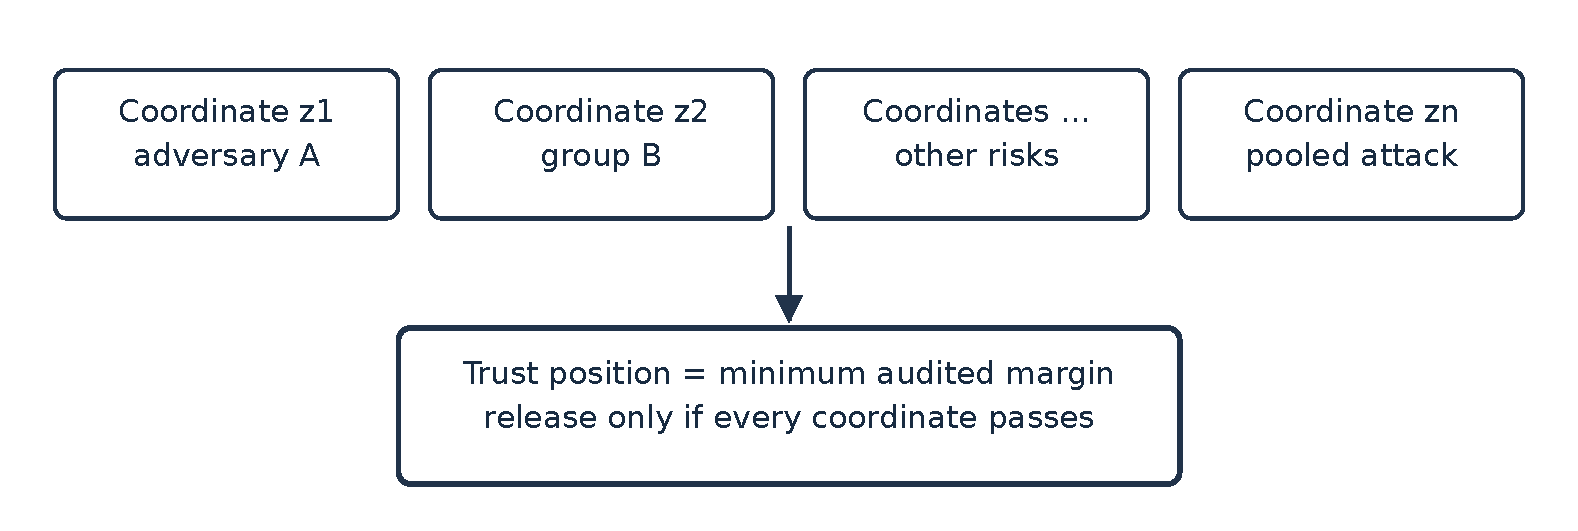
\includegraphics[width=.94\linewidth]{diagrams/trust_vector.pdf}
\caption{The $n$-dimensional trust position uses independently bounded risk coordinates $z_j=1-\overline r_j/\tau_j$. The labels illustrate declared coordinates, not numerical results.}
\label{fig:trust-vector}
\end{figure}


\subsection{The neural model and what its output means}

Encode a proposed release and its environment as $x(\theta)\in\mathbb R^d$:
mechanism parameters, sample fraction, key entropy and sparsity, auxiliary
information quality, number and overlap of prior releases, access controls,
population shifts and target-group indicators. All features must be available
\emph{before} certification and their provenance recorded. A transparent
baseline is a regularised logistic model; our nonlinear proposal model is
\begin{align}
 H_0&=x, &H_{\ell+1}&=\rho(H_\ell W_\ell+b_\ell),\quad 0\leq\ell<L,\\
 \widehat{\boldsymbol r}_{\phi}(x)
   &=\sigma(H_LW_{\rm out}+b_{\rm out})\in(0,1)^n,
 &\mathcal L(\phi)&=-\sum_{i,j}w_{ij}
  [y_{ij}\log\widehat r_{ij}+(1-y_{ij})\log(1-\widehat r_{ij})].
 \label{eq:neural-risk}
\end{align}
The \texttt{neural\_trust} module fixes $L=1$; \texttt{sentry\_r} makes $L$
configurable.
The label $y_{ij}$ is the \emph{observed success of an attack} on a separate
scenario draw, with a zero label for a failed or abstaining attack as specified
in the threat model. Unevaluated pairs have $w_{ij}=0$; repeated attacks sharing
one auxiliary file are clustered by file rather than treated as independent.
The sigmoid outputs are predicted attack frequencies, not audited margins or
probabilities that a release is safe, and no ordering of them across harm classes is implied.
Train on past mechanism--adversary scenarios, hold out whole populations,
release programmes and vintages, and keep the final audit draws out of all
training, tuning, calibration and feature selection. Compare log loss, Brier
score and reliability diagrams with the logistic and frequency baselines, both
overall and by group \citep{guo2017}. A calibration plot is a diagnostic, never a certificate
for the highest-risk individual.

The neural model proposes a \emph{finite} shortlist $\Theta_0$: it ranks
candidates by their largest predicted risk-to-tolerance ratio; utility enters
only the final choice among certified candidates. For each candidate and $j$, run $B_{\theta
j}$ fresh, conditionally identically distributed Bernoulli attacks and count
$K_{\theta j}$ successes. Fix the sample sizes before observing final outcomes.
With $M=|\Theta_0|n$ prespecified inspected coordinates,
define the exact one-sided bound
\begin{equation}
 \overline r_{\theta j}=
 \begin{cases}
 1,&K_{\theta j}=B_{\theta j},\\
 F^{-1}_{\mathrm{Beta}(K_{\theta j}+1,\,B_{\theta j}-K_{\theta j})}
      (1-\alpha/M),&K_{\theta j}<B_{\theta j}.
 \end{cases}\label{eq:neural-audit}
\end{equation}
Certification uses \eqref{eq:trust-position} and \eqref{eq:neural-audit}, never
the neural output. The final choice may maximise $U$ among certified candidates,
provided the shortlist was fixed without looking at these final audit draws.

Figure \ref{fig:neural-workflow} makes the separation between development
and final evidence explicit. The arrows into the final gate carry audit
bounds and tolerances; the network contributes only the fixed shortlist.
\begin{figure}[H]
\centering
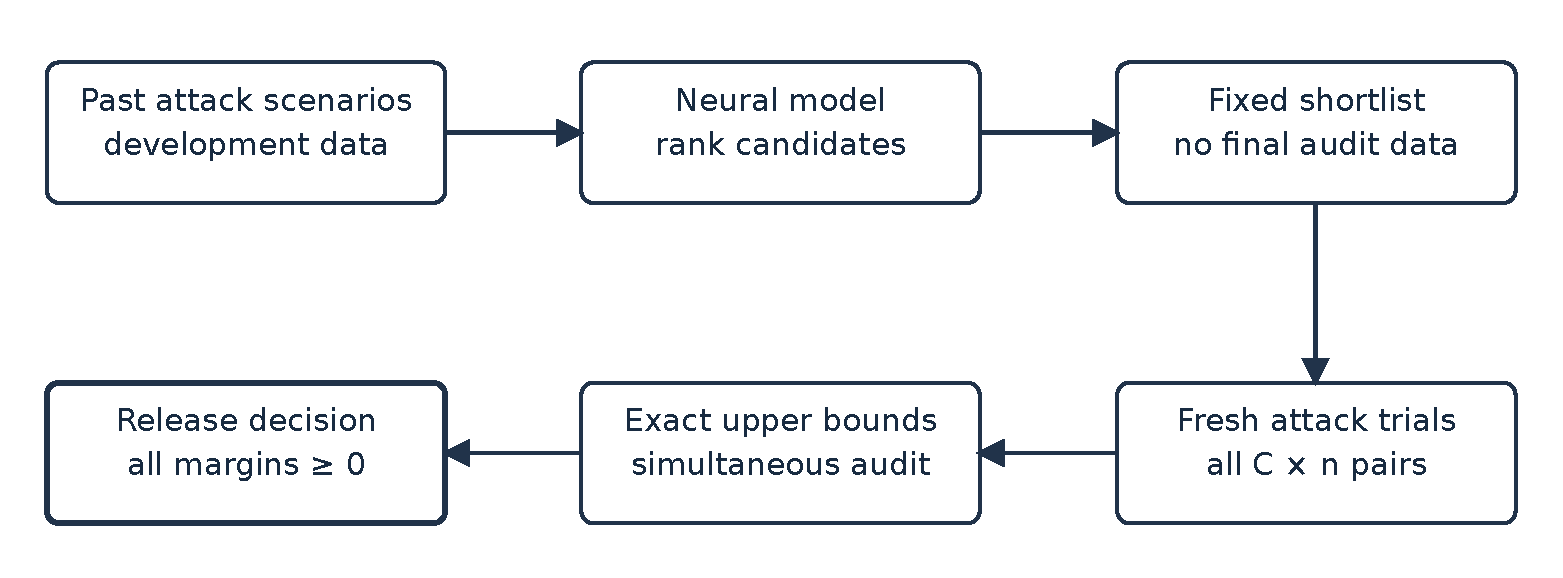
\includegraphics[width=.94\linewidth]{diagrams/neural_workflow.pdf}
\caption{The neural network ranks candidates; independent attack trials and exact simultaneous upper bounds decide. $C=|\Theta_0|$ and $n$ is the number of risk coordinates.}
\label{fig:neural-workflow}
\end{figure}


\begin{proposition}[Selection-safe finite-family certification]\label{prop:neural-gate}
Condition on development information $\mathcal D$ and its resulting finite
shortlist, candidate releases, scenarios and sample sizes. Suppose each final
audit count is $\mathrm{Binom}(B_{\theta j},r_j(\theta))$ conditional on
$\mathcal D$; auxiliary information sampled afresh is included in this
experiment, whereas fixed auxiliary information is conditioned upon. Then
with probability at
least $1-\alpha$, simultaneously for every inspected pair,
$r_j(\theta)\leq\overline r_{\theta j}$. Consequently the rule selecting any
candidate with $T(\theta)\geq0$ has probability at most $\alpha$ of certifying
a candidate whose risk exceeds a declared tolerance in any coordinate.
\end{proposition}
\begin{proof}
For one pair the event that the exact upper bound falls below the true risk
has probability at most $\alpha/M$ by inversion of the binomial lower-tail
test (Appendix \ref{app:neural}). A union bound over the $M$ pairs gives the
simultaneous statement, without requiring independence between pairs. On this
event every certified candidate satisfies $r_j(\theta)\leq\tau_j$ for all
$j$, regardless of which certified candidate the final rule selects.
Taking expectation over $\mathcal D$ gives the unconditional guarantee.
\end{proof}

If the release, attack, shortlist or group definitions change in response to
final outcomes, the conditional argument no longer applies. Freeze and restart
with untouched audit draws, or replace the fixed-sample bound by the anytime
procedure of the main text (the section on adaptive attacks and anytime-valid certification) with an explicit multiplicity
allocation. Binomial sampling covers attack-draw variability conditional on a
fixed population and mechanism. It does not cover uncertain input data, unknown
auxiliary sources, a stronger future attacker or distribution shift. Those are
separate scenario coordinates or require a stated outer uncertainty analysis.

\subsection{What changes as the dimension grows}

The number $d$ of input features and the number $n$ of risk coordinates are
different. For widths $q_0=d,q_1,\ldots,q_L,q_{L+1}=n$, a dense forward pass
costs $O(\sum_{\ell=0}^{L}q_\ell q_{\ell+1})$ operations per scenario and
stores $O(\sum q_\ell q_{\ell+1})$ parameters; a training epoch multiplies
the cost by the number of labelled scenarios. Sparse embeddings or shared
encoders can reduce cost when many groups share structure, but cannot supply
evidence in an unseen group. A full final audit over $C$ candidates and $n$
coordinates uses $Cn$ confidence bounds and, at zero observed successes in
every coordinate, needs at least
\begin{equation}
 B\geq\left\lceil\frac{\log(\alpha/(Cn))}{\log(1-\tau_{
 \min})}\right\rceil\label{eq:neural-budget}
\end{equation}
independent trials per coordinate to certify a common minimum tolerance
$\tau_{\min}$. This is necessary and sufficient when that coordinate has
zero successes; with successes, more trials can be needed. Thus computational
amortisation by a network
does not erase the statistical cost of many simultaneous guarantees.
For an $L$-Lipschitz risk function on $[0,1]^d$, even a direct grid at
accuracy $\epsilon$ uses order $(L/\epsilon)^d$ cells. Without such
regularity, finite observations alone cannot guarantee uniform pointwise
accuracy. Report learning curves against both $d$
and $n$; do not describe merely adding hidden units as solving this problem.

For stress testing, if the full law $Q_{\theta j}$ of the deployed attack
experiment is known to satisfy
$\mathrm{TV}(P_{\theta j},Q_{\theta j})\leq\delta_j$,
bounded attack success gives
$r_{Q_{\theta j}}(\theta)\leq r_{P_{\theta j}}(\theta)+\delta_j$.
A declared and justified
bound can therefore replace $\overline r_j$ by
$\min(1,\overline r_j+\delta_j)$. Estimating $\delta_j$ from a neural
embedding alone does not justify that guarantee. Out-of-scope feature values,
new linkage data and an unbounded shift require refusal and a new assessment.

The testable methodological contribution is the combination of an audited
margin vector, a neural search model, and an independent simultaneous audit
under adaptive choice of the final candidate. Neural prediction, binomial
bounds and neural calibration individually have extensive precedents
\citep{bates2021,guo2017}; the
claim here is about their stated division of labour for a release programme,
not an untested claim of superior empirical performance. The accompanying
\texttt{privacy\_risk.neural\_trust} module includes a seeded synthetic demonstration of the search
and audit interface. It cannot validate the existing tables in this paper.
An empirical extension must preregister targets and populations, compare the
network with the logistic and frequency baselines at fixed audit budgets,
report selective utility and worst-group failures, and rerun every pooled
attack on held-out real programmes.

\section{SENTRY-R: scenario-enriched neural triage for release review}\label{sec:sentry}

We name the implementable extension \emph{SENTRY-R}, shorthand for
scenario-enriched neural triage for release review. This names the specified
workflow, not a claim that its
components are individually new or that a fitted network has improved real
release decisions. Its separation of three data streams is central:
\emph{untrusted scenario proposals}, \emph{measured development attacks}, and
\emph{untouched final audits}. The implementation supports any finite input
dimension $d$ and any finite number $n$ of declared risk coordinates. A deeper
network predicts attack frequencies for search; it does not certify a release.

\subsection{LLM-assisted scenario expansion and evidence provenance}

Let $\mathcal F_t$ denote the information available before development round
$t$, including past mechanisms, validated scenario specifications and measured
attacks. A language model proposes descriptions and numeric scenario features
$Q_t=G_t(\mathcal F_t,\xi_t)$. A deterministic validator checks the predeclared
feature names and bounds and the scenario identifier. The calling code, not
the language model, writes the source metadata: the model name and the
SHA-256 hash of the exact prompt. The validator does
not treat free-form text or a language-model risk estimate as an observed
success. A separate attack evaluator then draws $Z_{ti}$ under the accepted
scenario and records $K_{tj}=\sum_{i=1}^{B_{tj}}s_j(Z_{ti})$, together with
its experiment identifier and sampling unit. The retraining history grows by
\begin{equation}
 \mathcal F_{t+1}=\mathcal F_t\vee\sigma\!\left(Q_t,\operatorname{valid}(Q_t),
 \{K_{tj},B_{tj},\operatorname{provenance}_{tj}\}_{j\in\mathcal J}\right).
 \label{eq:sentry-filtration}
\end{equation}
The language model can change which \emph{development} experiment is run next;
it does not directly change a network weight or label. Source identifiers,
scenario hashes and an explicit partition label make the update inspectable.
Treating repeated targets or auxiliary files as independent Bernoulli trials
would break the specified sampling model. Human review is still required to
establish whether a proposed adversary, harm definition and auxiliary source
are plausible and permissible.

Let $\mathcal D=\mathcal F_{t_*}$ be all such development information at a
chosen stopping time $t_*$, including model weights and hyperparameter
selection. A separate validation set holds out entire release programmes;
final audit draws are excluded from $\mathcal D$. Conditional on $\mathcal D$,
freeze the coordinate definitions, policy tolerances, $C$ shortlisted
candidates, the family error $\alpha$ and the planned sample sizes
$B_{\theta j}$. The implementation writes all of these, with a named
tolerance owner, an expiry date and every development evidence identifier,
into one hashed freeze record. The final audit reads $\alpha$ from that
record and refuses to run if the record has changed, if the expiry date has
passed, if any trial count differs from the plan, or if an audit evidence
identifier was used in development. An optional append-only ledger refuses a
second audit of the same freeze. These checks bind an audit to its freeze.
On their own they do not prove the order of events, since the freeze hash has
no key or trusted time stamp. An optional keyed ledger records a stronger
local history: each instrumented stage, from the language model's proposal through
review, measurement, training and freeze to the audit, is appended to one
hash-chained file, each entry signed with HMAC-SHA256 under a key the operator
holds, and an entry is refused unless the entries it depends on are already on
the chain. The same ledger holds each programme's error budget and debits
every recorded audit's $\alpha$ against it. New measurement entries also commit
the full measured row, so changed features or counts are refused when recording
a training artifact. These checks apply when provenance and proposal lineage
are retained. Base evidence, reviewer identities and evaluator authenticity
remain caller-controlled, and an operator can omit provenance or relabel data.
The audit debit occurs after outcomes are supplied; it does not prevent an
operator from obtaining or discarding outcomes outside the recorded path. A
service must reserve budget before draws, preserve every attempt and anchor
chain heads outside the operator's control. A key holder can otherwise rewrite
the file. Under the stated statistical assumptions, Proposition
\ref{prop:neural-gate} guarantee then applies even if the \emph{development}
sequence used an LLM adaptively, provided the conditional binomial model for
the untouched final draws holds. A final audit reused as development data, or
an LLM proposal generated from its outcomes, invalidates that conditioning.
Figure \ref{fig:sentry-loop} shows the implemented boundary. It reads from left
to right and then down. A scenario proposed by a language model passes a fixed
schema and a named review, and it can add a scenario but never an outcome. Only
counted development attacks train the deep proposal model, whose ranking fixes a
shortlist of candidate settings. Only the fresh final audit, with simultaneous
bounds over every coordinate, reaches the release decision. The note under the
first box states the rule the figure is there to show: proposal text never
supplies a training label or a release certificate.
\begin{figure}[tbp]
\centering
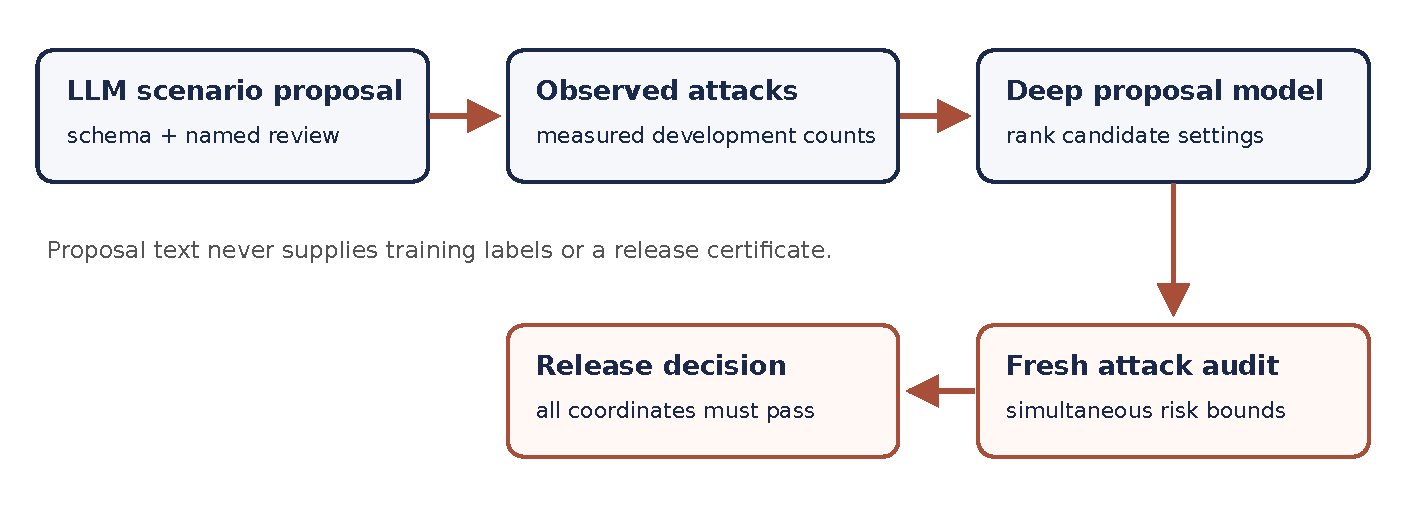
\includegraphics[width=0.95\linewidth]{diagrams/sentry_r_loop.pdf}
\caption{SENTRY-R development and decision boundary. The LLM's scenario proposal is checked against a fixed schema; only measured development attacks enter the deep model. Its ranking freezes a shortlist before a fresh, independent final audit.}
\label{fig:sentry-loop}
\end{figure}


\subsection{A deep model trained on counted attack outcomes}

The \texttt{privacy\_risk.sentry\_r} module provides a depth-$L$ fully connected
ReLU model with common width $q$, including the depth-zero logistic baseline.
Training features $x_i\in\mathbb R^d$ are standardised using \emph{training}
means and scales only. With $h_i^0=x_i$, for $\ell=0,\ldots,L-1$ define
\begin{equation}
 h_i^{\ell+1}=\rho(h_i^\ell W_\ell+b_\ell),\quad
 a_{ij}=\left(h_i^L W_{\mathrm o}+b_{\mathrm o}\right)_j,\quad
 p_{ij}=\sigma(a_{ij}),\quad \rho(z)=\max\{0,z\}.
 \label{eq:sentry-deep}
\end{equation}
For each observed development pair $(i,j)$ let $K_{ij}\in\{0,\ldots,B_{ij}\}$
be the count of successes in $B_{ij}\geq1$ trials. The implementation
minimises the binomial negative log likelihood, without its constant
combinatorial term, and a ridge term:
\begin{equation}
 \mathcal L(\phi)= -\frac{1}{B_\bullet}\sum_{i,j}
 \left[K_{ij}\log p_{ij}+(B_{ij}-K_{ij})\log(1-p_{ij})\right]
 +\frac{\lambda}{2}\sum_{\ell=0}^{L}\|W_\ell\|_F^2,
 \quad B_\bullet=\sum_{i,j}B_{ij}.
 \label{eq:sentry-count-loss}
\end{equation}
Here $W_L=W_{\rm o}$; a weight attached to trial count is appropriate only if
the count's sampling design was fixed without peeking at those outcomes. To
see exactly what is learned, assume $K\mid x,B\sim\mathrm{Binom}(B,\pi_j(x))$
with $B$ determined before outcomes. For a fixed $x,B$, the expected
unregularised loss minus its value at $p=\pi_j(x)$ is
\begin{equation}
 \frac{B}{B_\bullet}\,D_{\mathrm{KL}}
 \left(\mathrm{Bern}(\pi_j(x))\,\|\,\mathrm{Bern}(p)\right)\geq0.
 \label{eq:sentry-proper}
\end{equation}
Thus the ideal unrestricted conditional predictor is the attack success
frequency $\pi_j(x)$ on the \emph{development} distribution; finite data,
regularisation, optimiser error and population shift prevent equality in an
actual trained model. No neural output is a confidence limit on an individual
or a new population.

The model is fitted by backpropagation. With $P=(p_{ij})$, $K=(K_{ij})$ and
$B=(B_{ij})$, the output-logit derivative is $(B\odot P-K)/B_\bullet$, and the
hidden-layer gradients follow by the chain rule in the usual way
\citep[ch.~6]{goodfellow2016}. The package includes a finite-difference check of
the derivatives.

\subsection{Training, scale and falsification}

The network uses seeded mini-batches, Adam, gradient clipping and early
stopping on a separate held-out programme. Depth zero is trained on the same
counted outcomes as a logistic baseline. For $N$ development rows and $E$
epochs, the dense leading arithmetic order is
$O\{EN[dq+(L-1)q^2+qn]\}$ for $L\geq1$, with
$O\{dq+(L-1)q^2+qn\}$ weights; the logistic case has $O(ENdn)$
arithmetic. This is a computational scaling statement, not a statistical
sample-size promise. The final $Cn$ confidence bounds and independent attack
trials remain necessary whatever the prediction speed. Unknown groups and
out-of-domain features trigger a new assessment rather than an extrapolated
certificate.

A valid empirical evaluation must compare deep and logistic rankings at fixed
shortlist sizes and audit budgets on held-out \emph{real} programmes; report
log loss, Brier score, worst-group calibration, selected utility and false
gates; repeat pooled-vintage attacks; and show uncertainty across programmes.
This package currently provides a seeded synthetic end-to-end demonstration,
not such an evaluation. Table \ref{tab:sentry-synthetic} is regenerated by
\texttt{scripts/sentry\_r\_benchmark.py}. For each of ten seeds it draws
three disjoint programmes from one toy law: 320 training rows, 100 rows used
only for early stopping, and 2,000 test rows used only for the reported loss.
Both models train until 150 epochs pass without improvement, and no best
epoch reaches the cap. Trained to convergence, the logistic model has a
slightly lower test log loss than the three-layer model in all ten
replicates. The mean paired gap is smaller than the spread of either model
across replicates. The table shows that the pipeline runs, not that depth
helps. The test programmes come from the same law and feature range as the
training data, so they do not test shift.
\begin{table}[H]
\centering
\small
\caption{Synthetic SENTRY-R comparison over 10 seeded replicates of the toy law. Each replicate draws 320 training rows, 100 rows used only for early stopping (patience 150 epochs, cap 6000) and 2000 test rows used only for the reported losses. Entries are mean (standard deviation) across replicates; smaller is better. The last row is the paired deep-minus-logistic test log loss (range 0.0004 to 0.0050; deep lower in 0 of 10). These are not results on real release programmes.}
\label{tab:sentry-synthetic}
\begin{tabular}{lrrr}
\toprule
Proposal model & Test log loss & Test Brier score & Best epoch (range) \\
\midrule
Logistic & 0.2556 (0.0043) & 0.0727 (0.0017) & 404--898 \\
Three-layer ReLU & 0.2576 (0.0047) & 0.0735 (0.0018) & 79--402 \\
\midrule
Deep minus logistic & 0.0020 (0.0014) & & \\
\bottomrule
\end{tabular}
\end{table}



\section{Falsification and validation}\label{sec:falsify}

Reproducing the equations of Sections \ref{sec:setup} to \ref{sec:dp} in
software is an implementation check, not empirical validation. Evidence for the
scenario model must be capable of contradiction. We propose six tests, each
with a stated failure consequence, and report how the simulation of Section
\ref{sec:sim} performs against them.

\begin{enumerate}
\item \textbf{Linkage calibration.} Posterior probabilities from \eqref{eq:post}
must agree with held-out match frequencies within prespecified bands. Figure
\ref{fig:calib} shows the test passing for the correct model with a mean gap of
0.007 and failing for a misspecified covariate precision with a gap of 0.049,
while the two risk estimates differ by 0.007. Failure means the risk figure is not
supported, whatever its value.

\item \textbf{Population-frequency validation.} The model behind
\eqref{eq:rho} must predict held-out or externally benchmarked key frequencies.
In Section \ref{sec:sim} the fitted law recovers the mean population cell size
to within 1 per cent and the journalist risk to between 8 and 25 per cent, and
the direction of the error is conservative. Failure means the journalist figure
should be replaced by a bound.

\item \textbf{Adversary stress test.} A materially stronger plausible feature
set must not push the upper risk bound above $\tau$. In the simulation, an adversary whose
covariate is twice as precise raises the simulated risk by between 1 and 76 per
cent across the 45 settings of the grid, with a median of 40 per cent. This is
why the robust risk \eqref{eq:rob}, and not the nominal risk, is the coordinate
in Figure \ref{fig:frontier}. Capability and modelling are separate things, and
a second check records the difference: an adversary that keeps its information
but assumes the covariate is noisier than it is loses only 0.007 of its success
rate while its calibration gap grows sevenfold, so a risk figure alone will not
reveal the mistake. The record swapping lever described in Section
\ref{sec:sim} was removed on the same principle. Failure of the test means the
release fails or the scenario is revised in writing.

\item \textbf{Mechanism monotonicity.} Where stronger protection is claimed to
reduce risk, violations must be investigated rather than smoothed. Every row of
Table \ref{tab:kanon} violates the nominal bound on the supremum control, and
the investigation of that violation is Proposition \ref{prop:kanon}.

\item \textbf{Composition test.} Simulated joint attacks under \eqref{eq:joint}
must be compared with the marginal bound \eqref{eq:boole} and evaluated against
a programme tolerance. In Section \ref{sec:composition} the comparison fails by
a factor of 1.6 at two releases. Failure means the programme, not the release,
is the object that needs governing.

\item \textbf{Temporal transport.} An assessment must fail or be re-estimated
when new registers, linkage methods or data vintages move observed attack
performance outside its prespecified range. This is the test that the expiry
date $d$ in Definition \ref{def:thresh} enforces, and it is the only one of the
six that cannot be run at assessment time.
\end{enumerate}

\section{Operational protocol}\label{sec:protocol}

The governance record should follow five stages, in this order, with the output
of each written down before the next begins.

\begin{enumerate}
\item \textbf{Declare} the attack scenario $a$, the target set $T$, the harm
class $h$, the uncertainty set $H_a$ and the loss $\mathcal{L}$.
\item \textbf{Compute} the point estimate $\widehat{R}_a$, the bound
$\overline{R}_{1-\alpha}$ and the number of replicates $B$, with the dependence structure
of the replicates stated.
\item \textbf{Review} whether the declared scenario is plausibly conservative,
using the tests of Section \ref{sec:falsify}.
\item \textbf{Apply} the tolerance $\tau$ through the named owner $o$, using
rule \eqref{eq:admiss}.
\item \textbf{File} the complete record with the expiry date $d$ and evidence
sufficient to reproduce the computation.
\end{enumerate}

Exposure and harm remain distinct throughout. The risk $R_a$ measures the
probability of successful exposure; the tolerance $\tau(h)$ reflects the
consequence class, the legal duties and the public value of the release. The
owner owns the residual risk. The analyst owns the correctness of the
calculation. These are separate responsibilities and should sit with separate
people.

For a programme, two further items belong in the record: the joint attack
simulation under \eqref{eq:joint} with its own tolerance, and, where a formal
mechanism is used, the accountant's running total with the accounting method
named. Neither can be inferred from the single-release records.

\section{Discussion}\label{sec:disc}

The argument of this paper is that a release decision has three parts that
should be separately visible, and that most of the difficulty in practice comes
from collapsing them. Section \ref{sec:experiment} shows that the standard risk
measures are theorems about one linkage experiment, so that changing the
experiment changes the measure; Section \ref{sec:est} shows that the resulting
figure is an estimate whose uncertainty belongs in the decision rule; Section
\ref{sec:gov} shows that the tolerance is a policy quantity that a stated relative harm weight
already pins down. The two negative results are the ones with the most
immediate consequence for institutions. A $k$-anonymous release does not guarantee a risk of $1/k$ for the people in
it once the adversary holds anything beyond the key (Table \ref{tab:kanon}), and a programme of low-risk releases can be
attacked far above the bound its marginals imply (Table \ref{tab:comp}). Section \ref{sec:eval} shows what
the second costs on a release system rather than in a construction. On the
synthetic register, every suppression policy calibrated on one release leaves the
pooled programme above the 0.12 tolerance; only the noisy-count releases meet it,
at a large loss of loan-level utility.

Four limitations apply. First, the simulation is synthetic.
It establishes that the phenomena occur under a transparent data generating
process and that the estimators behave as the propositions say, and it cannot
establish the magnitudes an agency would see on its own register; those depend
on the auxiliary data actually available, which is exactly the quantity a
declared scenario has to guess. Second, the framework represents harm through a
scalar $c_h$ within a declared class $h$. Harms that fall on groups rather than
individuals, and harms that arise from correct inference about a population
rather than identification of a person, are outside it, and the second of these
is precisely what \citet{dwork2014} argue is not a privacy violation at all.
Third, the joint attack in Section \ref{sec:composition} is one pooling rule
among many. It gives a lower bound on what a pooling adversary achieves, so it
supports the negative result of Proposition \ref{prop:nopool}, but no
simulation can deliver the supremum over rules that a formal guarantee delivers
by construction. Fourth, the neural proposal model is illustrated only on
independent synthetic attack trials. Its output has no established calibration
or utility benefit on the credit and census data reported here, and the final
audit remains conditional on the declared attack scenario.

Four extensions look tractable. The frontier estimation in Section
\ref{sec:ru} could be given a proper inferential treatment, since the frontier is a functional of an estimated set and its selected point
is biased in the same way as any quantity chosen by maximising an estimate. The risk budget of Proposition
\ref{prop:budget} could be extended from the union event to a joint accountant
that admits dependence, which would need a composition theorem for
scenario-conditional risk under a stated dependence class. The implied tolerance
of Proposition \ref{prop:tau} could be estimated from revealed institutional
behaviour, since agencies have been making these decisions for decades and
their past choices identify $\kappa$ under the framework. And the calibration
test of Section \ref{sec:falsify} could be developed into a formal
specification test with a distribution under the null.

The recommendation is unchanged from the short version of this argument. Publish, alongside each release decision, the risk
estimate, the uncertainty bound and the number of replicates behind it, the
tolerance, the adversary specification, the mechanism setting, the named owner
and the expiry date. For a programme, publish the joint simulation as well. That
record does not remove judgement from the decision. It puts judgement in the
policy quantity where it belongs and leaves the probability calculation
reproducible and open to being proved wrong.

\subsection{What a release committee should take from this}

Three decisions follow from the argument, and they are the only three that need a
committee. The first is the tolerance, its accountable owner and its expiry date,
which Definition \ref{def:thresh} makes a record rather than a habit. The
second is whether that tolerance is asserted of each release or of the programme,
which Section \ref{sec:eval} shows is not a matter of wording: on the synthetic
register, at a tolerance of 0.12 and with the minimum cell count chosen by the
upper bound, the per-release reading of the same rule permits a release the
programme reading forbids, and the difference between them is
32{,}581 released loans against 23{,}068. The
third is the adversary specification, written down, so that the assumption can be
disagreed with explicitly instead of inherited silently.

A fourth choice is easy to miss because the arithmetic hides it. The measures of
Section \ref{sec:three} protect different people. The marketer measure is an
average over the released records, and a release can meet a tolerance on that
average while a particular record in it is identified with near certainty. The
prosecutor measure in its supremum form protects the most exposed record instead,
and the subgroup bounds of Section \ref{sec:eval} are the operational form of
the same idea. Which one an institution reports is an ethical choice about whose
protection the threshold is for, not a technical preference, and the framework
supports either as long as the committee says which it has chosen.

\subsection*{Data and code availability}

The numerical results and figures in the original sections are generated by
this repository's experiment pipeline, with the configuration and recorded
outputs in \texttt{artifacts-paper/}. The manuscript's numerical checks can be
run with \texttt{scripts/check\_paper\_numbers.py}; numerical reproducibility
is a separate claim from the new neural method. The new
\texttt{privacy\_risk.neural\_trust} module implements a vector risk
prediction, a finite-shortlist proposal and an independent simultaneous
binomial audit. Its seeded demonstration is synthetic and produces no inputs
to the original empirical tables or figures. Validation of neural ranking on
held-out real release programmes remains future work. The two public microdata
files described in Section \ref{sec:real} are loaded through the
\texttt{wooldridge} package by the original pipeline.

\subsection*{Acknowledgements}

An earlier version was prepared for the Workshop on Data Security and Privacy of
the Banco de Portugal and the Irving Fisher Committee, Lisbon, September 2026.
The views are the author's own.

\appendix

\section{Proofs}\label{app:proofs}

\begin{proof}[Proof of Proposition \ref{prop:recip}]
Condition on $S_t = 1$ and $K_a(X_t) = k$. By Assumption \ref{as:key} the
released key of every record equals its confidential key, and by Assumption
\ref{as:obs} the adversary observes $k$. The compatible set is therefore
$\{j \in I : K_a(X_j) = k\}$, which has cardinality $f_k$ by \eqref{eq:freq}
and contains $t$. By Assumption \ref{as:exch} the adversary's information is
invariant to permutations of that set, and by Assumption \ref{as:unif} it
selects each member with probability $1/f_k$. Exactly one member is correct,
so
\[
\Prob\{\delta_a = t \mid S_t = 1, K_a(X_t) = k, f_k\}
= \sum_{j=1}^{f_k} \frac{1}{f_k}\ind{j = t} = \frac{1}{f_k} . \qedhere
\]
\end{proof}

\begin{proof}[Proof of Proposition \ref{prop:kanon}]
By \eqref{eq:pros} and Proposition \ref{prop:recip}, $\sup_{t \in I}
R_{\mathrm{pros}}(t,\theta) = 1/\min_{k : f_k > 0} f_k$. Hence $\sup_t
R_{\mathrm{pros}} \leq \tau$ if and only if $\min_k f_k \geq 1/\tau$, and since
$f_k$ is an integer this is $\min_k f_k \geq \lceil 1/\tau \rceil$, which is the
definition of $k$-anonymity with $k = \lceil 1/\tau\rceil$.

For the failure claim, drop Assumption \ref{as:exch}. Let the release publish a confidential
variable $y$ alongside the key, let a key class have $f_k = k$ members with
distinct values of $y$, and let the adversary observe $z_t = y_t + \sigma \xi$ with $\xi$ standard normal and
$\sigma$ small relative to the within-class spacing of $y$. The posterior
\eqref{eq:post} concentrates on the member whose $y$ is nearest $z_t$, and as
$\sigma \downarrow 0$ the success probability of the maximum-posterior rule
tends to one, while $k$-anonymity holds for every $\sigma$. Therefore
$\sup_t R_a^{\mathrm{in}} > 1/k$ for all sufficiently small $\sigma$.
\end{proof}

\begin{proof}[Proof of Proposition \ref{prop:cert}]
With zero successes the one-sided Clopper--Pearson upper limit solves $(1 -
U)^B = \alpha$, giving $\overline{R}_{1-\alpha} = 1 - \alpha^{1/B}$ as in \eqref{eq:cp0}.
Then $\overline{R}_{1-\alpha} \leq \tau$ if and only if $\alpha^{1/B} \geq 1 - \tau$.
Taking logarithms, and noting $\log \alpha < 0$ and $\log(1-\tau) < 0$, this is
$B^{-1}\log\alpha \geq \log(1-\tau)$, that is $B \geq \log\alpha /
\log(1-\tau)$. Since $\log(1-\tau) = -\tau + O(\tau^2)$, the right side is
$-\log\alpha/\tau + O(1)$ as $\tau \downarrow 0$.
\end{proof}

\begin{proof}[Proof of Proposition \ref{prop:plugin}]
For any occupied key class, $f_k \leq F_k$ by \eqref{eq:freq}, hence $1/f_k
\geq 1/F_k$ pointwise, and monotonicity of expectation gives the first claim,
with equality if and only if $f_k = F_k$ almost surely for every class the
average touches. The second claim is Jensen's inequality applied to the convex
function $x \mapsto 1/x$ on $(0, \infty)$, which is strict unless $f_k$ is
degenerate.
\end{proof}

\begin{proof}[Proof of Proposition \ref{prop:point}]
At $R_a = \tau$, asymptotic symmetry of the estimator gives
$\Prob(\widehat{R}_a \leq R_a) \to 1/2$, so the point-estimate rule releases
with probability tending to $1/2$. A valid one-sided $(1-\alpha)$ upper bound
satisfies $\Prob\{R_a \leq \overline{R}_{1-\alpha}\} \geq 1 - \alpha$, hence
$\Prob\{\overline{R}_{1-\alpha} < R_a\} \leq \alpha$. At the boundary, release under
\eqref{eq:admiss} implies $\overline{R}_{1-\alpha} \leq \tau = R_a$, an event of
probability at most $\alpha$ up to equality conventions.
\end{proof}

\begin{proof}[Proof of Proposition \ref{prop:tau}]
On the frontier the problem is $\max_r \{\lambda\varphi(r) - c_h r\}$ over
$[\underline r, \overline r]$. The objective is strictly concave because
$\varphi$ is, so a maximiser exists and is unique. Its derivative is
$\lambda\varphi'(r) - c_h$, which is strictly decreasing; under
$\varphi'(\underline r) > \kappa > \varphi'(\overline r)$ with $\kappa = c_h /
\lambda$ it is positive at $\underline r$ and negative at $\overline r$, so the
maximiser is interior and solves $\varphi'(r) = \kappa$. Monotonicity of
$\tau^\star$ in $\kappa$ follows because $\varphi'$ is strictly decreasing, so
$\tau^\star = (\varphi')^{-1}(\kappa)$ is decreasing in $\kappa$.
\end{proof}

\begin{proof}[Proof of Proposition \ref{prop:exist}]
The feasible set $\Theta_\tau = \{\theta : \sup_{t}\overline{R}_{1-\alpha}(t,\theta) \leq
\tau\}$ is closed by lower semicontinuity of the constraint function, hence
compact as a closed subset of the compact $\Theta$, and nonempty by assumption.
An upper semicontinuous function attains its maximum on a nonempty compact set.
\end{proof}

\begin{proof}[Proof of Proposition \ref{prop:boole}]
Monotonicity gives $C_i \subseteq \bigcup_j C_j$ and hence $R_i \leq R_\cup$
for every $i$, so $\max_i R_i \leq R_\cup$. Boole's inequality gives $R_\cup
\leq \sum_i R_i$, and $R_\cup \leq 1$ always, which is the upper bound.
Attainment: if the events are nested, $C_1 \supseteq C_2 \supseteq \cdots$,
then $R_\cup = R_1 = \max_i R_i$. If they are disjoint and $\sum_i R_i \leq 1$,
then $R_\cup = \sum_i R_i$; if $\sum_i R_i > 1$, a standard overlapping
construction on $[0,1]$ with Lebesgue measure, placing $C_i$ as intervals that
cover $[0,1]$, gives $R_\cup = 1$.
\end{proof}

\begin{proof}[Proof of Proposition \ref{prop:nopool}]
Fix $m \geq 2$ and an integer $k \geq 1/\nu$. Let the sample consist of
$n = k^m$ units labelled by the vectors $x = (x_1, \dots, x_m) \in \{1, \dots,
k\}^m$, all present with certainty. Let release $i$ publish the key
$K_i(x) = (x_1, \dots, x_{i-1}, x_{i+1}, \dots, x_m)$, that is all coordinates
except the $i$th. Each key class of release $i$ contains exactly $k$ units, so
the release is $k$-anonymous and, under Assumptions \ref{as:key} to
\ref{as:unif}, $R_i = 1/k \leq \nu$.

Now let the adversary hold all $m$ releases and know the target's full label.
The candidate set from release $i$ is $\{x : K_i(x) = K_i(t)\}$, which is the
set of units agreeing with $t$ in all coordinates except possibly the $i$th.
The intersection over $i = 1, \dots, m$ of these sets is $\{t\}$, because a
unit in the intersection agrees with $t$ in every coordinate: for coordinate
$j$, membership in the candidate set of any release $i \neq j$ forces
$x_j = t_j$, and $m \geq 2$ guarantees such an $i$ exists. Hence
$\delta_a^{(m)}$ that selects the unique element of the intersection satisfies
$R_{\mathrm{pool}} = 1$. Since $\nu$ was arbitrary and
$(R_1, \dots, R_m) = (1/k, \dots, 1/k)$ can be made arbitrarily small while
$R_{\mathrm{pool}} = 1$, no function of the marginals can bound
$R_{\mathrm{pool}}$ from above.

For the final claim, let $A_i(t)$ be the candidate set of release $i$ and
$G_m(t) = \bigcap_{i \leq m} A_i(t)$, and suppose the adversary selects
uniformly from $G_m(t)$. Then $G_{m+1}(t) \subseteq G_m(t)$ and $t \in G_m(t)$
for every $m$, so $1/|G_{m+1}(t)| \geq 1/|G_m(t)|$ pathwise and taking
expectations gives monotonicity. Since $G_m(t) \subseteq A_i(t)$ for each
$i \leq m$, the same argument gives $R_{\mathrm{pool}} \geq \max_{i \leq m}
\E[1/|A_i(t)|] = \max_i R_i$.
\end{proof}

\begin{proof}[Proof of Proposition \ref{prop:budget}]
The objective is strictly concave and the constraint set is compact and convex,
so a unique maximiser exists. Since $\varphi$ is increasing, the constraint
binds. The Lagrangian is $\sum_i w_i\varphi(r_i) - \mu(\sum_i r_i -
\tau_{\mathrm{prog}})$ and the first-order conditions are $w_i\varphi'(r_i) =
\mu$ for every $i$, which is \eqref{eq:water}; concavity makes them sufficient.
For $\varphi = \log$ the conditions read $w_i / r_i = \mu$, so $r_i \propto
w_i$, and the constraint fixes the constant at $\tau_{\mathrm{prog}}/\sum_j
w_j$. For $\varphi(r) = a + b r^{\gamma}$ with $b < 0$ and $\gamma < 0$, which
is increasing and strictly concave on $(0,\infty)$, we have $\varphi'(r) = b
\gamma r^{\gamma - 1}$, so \eqref{eq:water} reads $w_i r_i^{\gamma - 1} =
\mu / (b\gamma)$ and hence $r_i \propto w_i^{1/(1-\gamma)}$, which is
\eqref{eq:power}.
\end{proof}

\begin{proof}[Proof of Proposition \ref{prop:attack-threshold}]
At posterior probability $p$, acting has expected payoff
$V(p)=ph-(1-p)c_f-c_a=p(h+c_f)-(c_f+c_a)$. Since $h+c_f>0$,
$V(p)\ge0$ if and only if $p\ge(c_f+c_a)/(h+c_f)$. If this ratio exceeds
one, no posterior below certainty justifies the attack, which gives the truncation
in \eqref{eq:attack-threshold}.
\end{proof}

\begin{proof}[Proof of Proposition \ref{prop:anytime}]
For fixed $u\in(0,1)$, the Bernoulli likelihood ratio through time $B$ between
risk $u$ and risk $r_0$ is a nonnegative $r_0$-martingale with initial value
one. Integrating these likelihood-ratio martingales against the
$\mathrm{Beta}(a,b)$ density preserves the martingale property by Tonelli's
theorem and gives exactly \eqref{eq:eprocess}. Ville's inequality for a
nonnegative martingale yields \eqref{eq:ville}. The event that $r_0$ exits
$\mathcal C_B$ at some time is the event that $E_B(r_0)\ge1/\alpha$ at some
time, so its probability is at most $\alpha$.
\end{proof}

\begin{proof}[Proof of Proposition \ref{prop:dpbound}]
Let $x$ and $x'$ be the databases in which $H$ is true and false respectively;
they differ in one individual's record, so they are neighbouring, and by
hypothesis the remaining records have the same distribution under both. For any
observed output set $E$ of positive probability, \eqref{eq:dp} with
$\delta_{\mathrm{dp}} = 0$ gives the likelihood ratio bound
$\Prob\{M(x) \in E\} / \Prob\{M(x') \in E\} \leq e^\varepsilon$. Bayes' rule in odds form gives
\[
\frac{\Prob(H \mid M \in E)}{1 - \Prob(H \mid M \in E)}
= \frac{p}{1-p}\cdot\frac{\Prob\{M(x) \in E\}}{\Prob\{M(x') \in E\}}
\leq \frac{p}{1-p}e^{\varepsilon} ,
\]
and solving for $\Prob(H \mid M \in E)$ gives \eqref{eq:dppost}. With
$\delta_{\mathrm{dp}} > 0$ the same steps give the exact bound
\[
\frac{\Prob(H \mid M \in E)}{1 - \Prob(H \mid M \in E)}
\leq \frac{p}{1-p}\Bigl(e^{\varepsilon}
+ \frac{\delta_{\mathrm{dp}}}{\Prob\{M(x') \in E\}}\Bigr) ,
\]
which is unbounded for rare $E$, so no uniform posterior bound holds when
$\delta_{\mathrm{dp}} > 0$. With probability at least
$1 - O(\delta_{\mathrm{dp}}/(1-e^{-\varepsilon}))$ over outputs, a bound of the
form \eqref{eq:dppost} holds with a slightly inflated $\varepsilon$
\citep{kasiviswanathan2014}.
\end{proof}

\section{Expanded derivations}\label{app:derivations}

This appendix expands the calculations used in the text, so that each reported
quantity can be reconstructed without treating an intermediate identity as
given.

\subsection{From joint success to membership-conditional risk}

Let $A_t=\{\delta_a(Z_t,Y_\theta)=t\}$ and $B_t=\{S_t=1\}$. Since a released
record cannot equal an unsampled target, $A_t\subseteq B_t$, and
\begin{equation}
R_a^{\mathrm{unc}}(t,\theta)
 =\Prob(A_t\cap B_t\mid\mathcal{B}_a)
 =\Prob(A_t\mid B_t,\mathcal{B}_a)\Prob(B_t\mid\mathcal{B}_a)
 =\pi_t R_a^{\mathrm{in}}(t,\theta),
\end{equation}
which is \eqref{eq:factor}. If the auxiliary information changes the adversary's
belief about membership, the last factor is $\Prob(B_t\mid\mathcal{B}_a)$ and not
the design probability $\pi_t$; using $\pi_t$ requires that $\mathcal{B}_a$ carry
no information about who was sampled.

\subsection{Bayesian linkage from comparison vectors}

Let $\gamma_{tj}=\gamma(Z_t,Y_j)$ be a comparison vector, and write
$m(\gamma)=p(\gamma\mid H_{tj}=1)$ and $u(\gamma)=p(\gamma\mid H_{tj}=0)$ for its
density under a match and a non-match, with likelihood ratio
$\Lambda_{tj}=m(\gamma_{tj})/u(\gamma_{tj})$. Under the usual assumptions that the fields of a comparison vector are
conditionally independent given the match status \citep{fellegi1969}, and that the
comparison vectors of distinct candidates are conditionally independent of one
another, Bayes' theorem and division by $\prod_\ell u(\gamma_{t\ell})$ give
\begin{equation}
p_{tj}=\frac{q_{tj}\Lambda_{tj}}
 {q_{t0}\Lambda_{t0}+\sum_{\ell\in I}q_{t\ell}\Lambda_{t\ell}},
\end{equation}
where $\Lambda_{t0}=1$, because under the no-match hypothesis every candidate is
scored by its non-match density and the division leaves one. This is
\eqref{eq:post} with $L=\Lambda$. Exact exchangeable matching is the case
of equal likelihood and prior weight on each of the $f_k$ compatible records and
zero weight elsewhere, giving $1/f_k$ for each. For two candidates,
\begin{equation}
\frac{p_{tj}}{p_{t\ell}}
=\frac{q_{tj}}{q_{t\ell}}\cdot\frac{L_{tj}}{L_{t\ell}} ,
\label{eq:posterior-odds-link}
\end{equation}
so the reciprocal-frequency figure is valid only when both ratios equal one inside
the key class. Equation \eqref{eq:posterior-odds-link} is where informative side
information enters.

\subsection{Journalist risk under binomial thinning}

Conditional on $F_k=v$, Bernoulli sampling gives $f_k\mid F_k=v\sim
\mathrm{Binomial}(v,\pi)$, so $\Prob(F_k=1,f_k=1)=\pi\Prob(F_k=1)$ and
$\Prob(f_k=1)=\sum_{v\ge1}v\pi(1-\pi)^{v-1}\Prob(F_k=v)$. Dividing the first by
the second gives \eqref{eq:rho}. For a parametric frequency law $g(v;\eta)$ the
plug-in estimator is
\begin{equation}
\widehat\rho_k=
\frac{\pi g(1;\widehat\eta)}
 {\sum_{v\ge1}v\pi(1-\pi)^{v-1}g(v;\widehat\eta)} ,
\end{equation}
and the analyst must carry the uncertainty in $\widehat\eta$ through
\eqref{eq:delta-risk}, or refit $g$ inside each replicate.

\subsection{Exact binomial bounds and simultaneous control}

If $X=\sum_b C_t^{(b)}=x$, the one-sided Clopper--Pearson upper endpoint is
\begin{equation}
\overline{R}_{1-\alpha}(x,B)=
\mathrm{Beta}^{-1}_{1-\alpha}(x+1,B-x),\qquad x<B,
\label{eq:cp-general}
\end{equation}
and one when $x=B$, where $\mathrm{Beta}^{-1}_q(a,b)$ is the $q$th quantile of a
beta distribution. At $x=0$ the beta distribution function is $F(u)=1-(1-u)^B$,
so $F(\overline{R})=1-\alpha$ recovers \eqref{eq:cp0}.

If $T$ holds $q$ targets and the decision uses their maximum, separately valid
$(1-\alpha)$ intervals do not give a $(1-\alpha)$ file-level statement. Bonferroni control uses targetwise error $\alpha/q$. Section \ref{sec:kanon} needs
the lower form, since it reports the worst target, so writing
$\underline{R}_{\alpha/q,t}$ for a one-sided lower limit,
\begin{equation}
\Prob\left\{R_t\ge \underline{R}_{\alpha/q,t}\ \text{for every }t\in T\right\}
\ge 1-\sum_{t\in T}\frac{\alpha}{q}=1-\alpha ,
\label{eq:bonf}
\end{equation}
and the same argument gives the upper form when the decision uses a maximum.
This is conservative but valid without independence, and it is what Section
\ref{sec:kanon} uses for the worst target. A max-statistic bootstrap can replace
it when the resampling scheme preserves dependence across targets
\citep{efron1993}.

\subsection{Nested estimator for simulation and input uncertainty}

Draw outer replicates $s=1,\dots,S$. In each, redraw the confidential sample
according to its design, refit any auxiliary model, apply the mechanism, and run
$B_s$ conditional attacks. With $\widehat R_s=B_s^{-1}\sum_b C_{sb}$ and
$\overline R=S^{-1}\sum_s \widehat R_s$, an analysis-of-variance decomposition is
\begin{equation}
\widehat V_{\mathrm{within}}
 =\frac1S\sum_{s=1}^S\frac{\widehat R_s(1-\widehat R_s)}{B_s},\qquad
\widehat V_{\mathrm{between}}
 =\frac{1}{S-1}\sum_{s=1}^S(\widehat R_s-\overline R)^2
   -\widehat V_{\mathrm{within}},
\end{equation}
the second truncated at zero when the finite estimate falls slightly negative.
The variance of $\overline R$ is then approximately
$(\widehat V_{\mathrm{between}}+\widehat V_{\mathrm{within}})/S$ for independent
outer replicates. Percentile or studentised outer bootstrap bounds avoid relying
on normality near zero. Section \ref{sec:nested} reports both terms.

\subsection{Tangency and boundary cases}

On a differentiable frontier $u=\varphi(r)$, maximise
$J(r)=\lambda\varphi(r)-c_hr$. Then
\begin{equation}
J'(r)=\lambda\varphi'(r)-c_h,\qquad
J''(r)=\lambda\varphi''(r)<0,
\end{equation}
so the first-order condition is sufficient and gives $\varphi'(r)=c_h/\lambda$.
If $c_h/\lambda\ge\varphi'(\underline r)$ the optimum is the safest boundary
$\underline r$; if $c_h/\lambda\le\varphi'(\overline r)$ it is the highest-risk
boundary $\overline r$. These cases complete Proposition \ref{prop:tau} when its
interiority condition fails.

For the programme allocation, allow $r_i=0$ and attach multipliers $\xi_i$ to the
non-negativity constraints. The Karush--Kuhn--Tucker conditions are
\begin{equation}
w_i\varphi_i'(r_i)-\mu+\xi_i=0,\quad \xi_i r_i=0,\quad
\mu\Big(\tau_{\mathrm{prog}}-\sum_i r_i\Big)=0,\quad \mu,\xi_i\ge0 ,
\end{equation}
so active releases equalise weighted marginal value, and a release receives zero
budget only when its marginal value at zero is no greater than the constraint multiplier
\citep{boyd2004}. This is the general form behind \eqref{eq:water}.

\subsection{Predictive value of an alleged relationship}

Let $D$ be the event that a stated relationship holds and $A$ the event that the
adversary alleges it. Bayes' theorem gives
\begin{equation}
\Prob(D\mid A)=\frac{p s}{p s+(1-p)(1-q)} ,
\qquad p=\Prob(D),\ s=\Prob(A\mid D),\ q=\Prob(A^c\mid D^c) ,
\label{eq:ppv}
\end{equation}
the sensitivity $s$ and specificity $q$ of the allegation. The quantity that
matters for harm is the left side, not $s$. When $p$ is small, as it is for
borrower--lender pairs, a specificity close to one still leaves a modest
predictive value, and Section \ref{sec:credit} reports the four cells of the
table so that \eqref{eq:ppv} can be checked as an identity rather than believed.

\subsection{Residual disclosure from published totals}

Let cells $c$ carry published totals $T_c=\sum_b x_{bc}$, where $x_{bc}$ is
contributor $b$'s amount. Stacking the published totals gives a linear system
$Ax=T$. A contribution $x_{bc}$ is determined by the release if and only if it is constant
on the feasible set $\{x : Ax=T,\ x\ge 0\}$ intersected with whatever else the
adversary knows, which for a participating institution includes its own row. The
non-negativity constraint is not decoration: it is what makes a zero total
disclosive, and it is what linear-programming attacks on suppressed tables
exploit. Two familiar cases follow at once. A cell with one contributor gives
$x_{bc}=T_c$. A cell with two contributors gives the other's amount to either of
them by subtraction. Requiring three contributors per published cell removes both, which is why that
rule is standard. Counting those two cases gives a lower bound on what the release
determines, not the whole of it, and it does not address the differencing attack
below.

\subsection{Differencing across consecutive releases}

Let $n_{c,m}$ and $T_{c,m}$ be the count and total published for cell $c$ in month
$m$. If $n_{c,m+1}-n_{c,m}=1$ and exactly one relationship moved, the arriving
amount is $T_{c,m+1}-T_{c,m}$. The adversary does not observe the number of moves.
Under a model in which arrivals $A$ and departures $D$ are independent Poisson
counts with mean $\lambda$, the posterior that an observed unit change came from a
single move is
\begin{equation}
\Prob(A=1,D=0\mid |A-D|=1)
=\frac{\Prob(A=1)\Prob(D=0)}
 {\sum_{|a-d|=1}\Prob(A=a)\Prob(D=d)} .
\label{eq:diffpost}
\end{equation}
The inference is therefore probabilistic, and its strength falls as the cell
becomes busier. Section \ref{sec:credit} evaluates \eqref{eq:diffpost} on the
simulated register.

\section{Simulation details}\label{app:sim}

\paragraph{Generation.} District and occupation categories are drawn from
distributions with probabilities proportional to $j^{-0.9}$ and $j^{-0.8}$
respectively, which produces the skewed cell sizes and the population uniques
reported in Section \ref{sec:sim}. Ages are drawn uniformly on $[18, 88)$ and
then thinned towards younger ages, so that the oldest bands are the sparse ones.
All draws use a single seeded generator.

\paragraph{Attack.} Targets are drawn uniformly with replacement from the
released records, except in the per-target experiment of Section
\ref{sec:kanon}, where each named target is attacked 250 times. The reported
lower bound for the worst target is the one-sided Clopper--Pearson limit from
those 250 replicates, taken at $0.05$ divided by the number of targets examined,
because that target is selected on its own estimate.
The adversary blocks on the target's district and sex, which it observes without
error. Within the block it evaluates the likelihood of the observed age band and
occupation group under the error model that generated them, with the neighbour
count of each candidate band handled so that the declared model and the
generating model agree at the boundary bands, and multiplies by the normal
density of the noisy covariate. It selects the maximum-posterior candidate and
abstains only when the total likelihood vanishes. Replicates within a setting
are independent draws of the target and of the adversary's information, so
\eqref{eq:mc} and the Clopper--Pearson bound apply to that draw, conditional on
the realised sample and mechanism output. They do not cover sampling
variability, and an institution reusing one auxiliary file across replicates
would not have even this much independence.

\paragraph{Grid and frontier.} The 45 mechanism settings are evaluated with
1,200 replicates each for both members of the uncertainty set, and the robust
risk is the larger point estimate with its own bound. Utility is the negative of
the average of three root mean squared errors, for the mean of $y$ by district,
by five-year age band and by occupation, each computed against the population
truth over target categories that the release can report with at least three
records and normalised by the standard deviation of $y$, plus a penalty of 0.5
times the average share of target categories left unreportable. Age and
occupation estimates are formed from the released classification, so a release
with 20-year bands or three occupation groups can only supply a piecewise
constant answer to an analysis stated at five-year bands or twelve occupations.
The frontier is the nondominated subset in the plane of the risk bound and this
utility. In the allocation of Section \ref{sec:composition} the fitted curve is
evaluated on $(0, \tau_{\mathrm{prog}}]$ with a numerical lower bound of
$10^{-3}$ on each share, which is inactive at the reported optimum.

\paragraph{Credit register.} The register of Section \ref{sec:credit} draws
borrowers with a sector, region and size class, gives each between one and four
lending relationships with larger firms holding more, and draws exposures
lognormally within size class and arrears at rates that vary by sector and size.
Six monthly vintages are generated by giving each relationship a start month and a
duration. The linkage attack blocks on region, requires an exact match on the
sector and size class, and multiplies by the density of a reading of log exposure
with standard deviation 0.6. Success is scored at the relationship, so recovering a
different relationship of the correct borrower counts as a failure; the
borrower-level figure is reported beside it. The published aggregates are totals by
region, sector and size class, and the differencing comparison uses the counts of
those cells across consecutive vintages, which is a separate lever from the
minimum cell count applied to the loan-level file.

\paragraph{Composition.} The four releases share one sample, so all dependence
between them is the dependence an agency would face when publishing several
products from one collection. Candidate sets are the key classes of each
release after suppression. A target suppressed from a release contributes zero
to that release's marginal risk and does not narrow the intersection, so the
pooled figure is what an adversary achieves using the releases that contain the
target. Reported marginal and pooled risks are means of $1/|A_i(t)|$ and
$1/|G_m(t)|$ over the same 20,000 targets rather than Bernoulli draws, which
removes selection noise without changing the estimand.

\section{Mathematical details for the audited margin vector}\label{app:neural}

\paragraph{Exploratory real-data runs.} The repository also holds a
state-held-out pilot of the proposal model on the public Census file and a later
comparison of linear, neural and quadratic proposers on the same file
(\texttt{scripts/realdata\_neural\_pilot.py} and
\texttt{scripts/realdata\_neural\_comparison.py}). Their linear baselines were
not trained to convergence and their differences lie within bootstrap intervals,
so they are not evidence for or against the procedure, and nothing in this paper
rests on them.

\paragraph{Experiment and estimand.}
Let $\mathcal D$ contain all development observations, candidate generation,
neural fitting, tuning, scenario definitions and proposed releases. Conditional
on $\mathcal D$, the shortlist $\Theta_0$, its cardinality $C$, and all
sample sizes $B_{\theta j}\geq1$ are fixed. An audit draw $Z_{\theta ji}$
includes the target, auxiliary data when freshly sampled, and any randomness
in the declared attack. The measurable success indicator
$S_{\theta ji}=s_{\theta j}(Z_{\theta ji})$ is one exactly when the declared
harm criterion is met. For fixed $(\theta,j)$ assume the draws are identically
distributed and independent conditional on $\mathcal D$, with law
$P_{\theta j}$. Thus
\begin{equation}
 r_j(\theta)=\int s_{\theta j}(z)\,dP_{\theta j}(z),\qquad
 K_{\theta j}=\sum_{i=1}^{B_{\theta j}}S_{\theta ji}\mid\mathcal D
 \sim\operatorname{Binom}(B_{\theta j},r_j(\theta)).
 \label{eq:neural-experiment}
\end{equation}
The risk is conditional on a frozen release and on the audit design. If target
records or auxiliary files are reused, the resulting dependent observations
must be treated as one sampling unit or justified by another valid confidence
procedure. Independence across distinct $(\theta,j)$ pairs is unnecessary.
For a finite population sampled without replacement, the binomial assumption
is inappropriate unless the attack design supplies independent replacement
draws; a hypergeometric or design-based bound is needed instead.

\paragraph{Exact inversion.}
Write $b=B_{\theta j}$, $k=K_{\theta j}$,
$\gamma=\alpha/(Cn)$, and
$F_p(k)=\sum_{t=0}^{k}\binom{b}{t}p^t(1-p)^{b-t}$. For $k<b$,
$F_p(k)$ is continuous and strictly decreasing in $p\in(0,1)$.
The upper endpoint $u(k)$ is the unique solution of $F_{u(k)}(k)=\gamma$;
set $u(b)=1$. The binomial--beta identity gives
\begin{equation}
 F_p(k)=1-I_p(k+1,b-k),\qquad
 u(k)=F^{-1}_{\operatorname{Beta}(k+1,b-k)}(1-\gamma).
 \label{eq:neural-inversion}
\end{equation}
For any fixed true $p$, the event $\{u(K)<p\}$ is a lower-tail set of
integer counts: by monotonicity it equals $\{F_p(K)<\gamma\}$, apart from
the harmless equality boundary. If $k_*$ is the largest count in this set,
$\Pr_p\{u(K)<p\}=F_p(k_*)<\gamma$; if the set is empty the probability is
zero. Hence $\Pr_p\{p\leq u(K)\}\geq1-\gamma$ for every $p\in[0,1]$.
The possible strict inequality reflects the discreteness of the count.

\paragraph{Familywise selection.}
Define the event
\begin{equation}
 E=\bigcap_{\theta\in\Theta_0}\bigcap_{j\in\mathcal J}
 \{r_j(\theta)\leq\overline r_{\theta j}\}.
 \label{eq:neural-good-event}
\end{equation}
Conditional on every development history for which the assumptions hold,
$\Pr(E^c\mid\mathcal D)\leq\sum_{\theta,j}\gamma=\alpha$.
Any measurable decision rule $\widehat\theta$ using the complete vector of
final bounds, including the choice of the greatest utility among accepted
candidates, satisfies the deterministic implication
\begin{equation}
 E\ \Longrightarrow\
 \bigl[\widehat\theta\text{ accepted}\bigr]\ \Longrightarrow\
 \max_{j\in\mathcal J}\frac{r_j(\widehat\theta)}{\tau_j}\leq1.
 \label{eq:neural-implication}
\end{equation}
The probability of a false certification is therefore at most $\alpha$
conditionally and, by $\Pr(E^c)=\E[\Pr(E^c\mid\mathcal D)]$, unconditionally.
This is a frequentist guarantee for the declared finite family; it is not a
posterior probability that a particular accepted release is safe. An audit
outcome used to add candidates, alter scenarios, retrain the network or select
sample sizes destroys the conditioning argument unless a separate sequential
or adaptive design is proved valid.

\paragraph{Budget and an illustrative calculation.}
At $k=0$, equation \eqref{eq:neural-inversion} simplifies to
$u(0)=1-\gamma^{1/b}$. Consequently $u(0)\leq\tau$ if and only if
$(1-\tau)^b\leq\gamma$, equivalently
\begin{equation}
 b\geq\left\lceil\frac{\log\gamma}{\log(1-\tau)}\right\rceil.
 \label{eq:neural-budget-proof}
\end{equation}
For illustration only, $C=4$, $n=2$, $\alpha=0.05$ and $\tau=0.12$ give
$\gamma=0.00625$ and $b=40$. The zero-success endpoint is approximately
$0.11916$ at $b=40$, but approximately $0.12202$ at $b=39$.
These numbers do not establish the risk of any real release. The total number
of attack trials is $\sum_{\theta,j}B_{\theta j}$; when each of $Cn$ pairs
uses the same $b$, it is $Cnb$. For small $\tau$,
$-\log(1-\tau)=\tau+O(\tau^2)$, so the zero-success requirement grows as
$\log(Cn/\alpha)/\tau$ per pair. The neural output dimension changes this
multiplicity even when its input feature dimension $d$ stays fixed.

\paragraph{Neural objective and its limits.}
Let $\pi_j(x)=\Pr(Y_j=1\mid X=x)$ in the development distribution. For a
positive weight $w_j(x)$ depending only on $x$ and $j$, the conditional
expected binary cross entropy at a predicted probability $q$ is
\begin{equation}
 \ell_x(q)=-w_j(x)[\pi_j(x)\log q+(1-\pi_j(x))\log(1-q)],
 \quad \ell_x'(q)=w_j(x)\frac{q-\pi_j(x)}{q(1-q)},
 \label{eq:neural-proper}
\end{equation}
with $\ell_x''(q)>0$ at its unique minimum $q=\pi_j(x)$ whenever
$0<\pi_j(x)<1$. Outcome-dependent weights instead change that minimiser.
The implemented one-hidden-layer ReLU model is fitted by ordinary
backpropagation of this objective \citep[ch.~6]{goodfellow2016}; the gradients are
textbook ones, and fitting does not make the predictions exact. Write $W_1$ and
$W_2$ for its fitted input-to-hidden and hidden-to-output weight matrices. Then
ReLU's Lipschitz constant of one and sigmoid's scalar derivative at most
$1/4$ give the predictor sensitivity bound
$\|\widehat{\boldsymbol r}(x)-\widehat{\boldsymbol r}(x')\|_2
\leq\|W_2\|_2\|W_1\|_2\|x-x'\|_2/4$.
It controls changes in \emph{predictions}, not errors relative to actual
risks, and is no substitute for the audit.

\paragraph{The input dimension.}
Suppose, as an additional assumption, the true conditional risk is
$L$-Lipschitz in $\|\cdot\|_\infty$ on $[0,1]^d$. A grid of spacing
$h\leq\epsilon/L$ lets a value at a nearby grid point approximate the
true risk to within $\epsilon$, requiring at most
$(1+\lceil L/\epsilon\rceil)^d$ grid points. Estimating those values adds
sampling cost at each point; the grid count alone already grows exponentially
in $d$. If no regularity links unsampled inputs to observed inputs, two risk
functions can agree on every observed feature vector and disagree arbitrarily
at an unobserved vector, so there is no distribution-free uniform interpolation
guarantee. Structural assumptions may help prediction, but the finite-family
audit guarantee above does not rely on them.

\paragraph{Distribution shift.}
Using $\mathrm{TV}(P,Q)=\sup_A|P(A)-Q(A)|$ on the complete audit-draw space,
the layer-cake representation for any success function $0\leq s\leq1$ yields
$|\E_Qs-\E_Ps|\leq\mathrm{TV}(P,Q)$. If a justified deterministic bound
$\mathrm{TV}(P_{\theta j},Q_{\theta j})\leq\delta_{\theta j}$ holds for
all inspected pairs, a simultaneous deployed-risk bound is
\begin{equation}
 \overline r^{\rm deploy}_{\theta j}
 =\min\{1,\overline r_{\theta j}+\delta_{\theta j}\},\qquad
 T^{\rm deploy}(\theta)=\min_j\left(1-
 \frac{\overline r^{\rm deploy}_{\theta j}}{\tau_j}\right).
 \label{eq:neural-shift}
\end{equation}
The same familywise probability applies because the TV inequality holds
pointwise on the simultaneous coverage event. A TV estimate, itself uncertain,
needs its own valid upper bound and error allocation. A distance between neural
feature embeddings alone cannot establish a TV bound on the full experiment.

\section{SENTRY-R derivations and adaptive development}\label{app:sentry}

\paragraph{Gradients.} The depth-$L$ network is fitted by ordinary
backpropagation of the count loss \eqref{eq:sentry-count-loss}. The only
non-standard term is the output-logit derivative, $b\sigma(a)-k$ for a count of
$k$ successes in $b$ trials, which follows from the chain rule; the rest is
textbook \citep[ch.~6]{goodfellow2016}, and the package checks the derivatives
by finite differences. Adam changes the update rule, not the gradients.

\paragraph{Adaptive proposal rounds and a fixed final experiment.}
A language model, human analyst or hyperparameter search may use the measured
\emph{development} history repeatedly. Let $T$ be an almost surely finite
stopping time for that history, and condition on $\mathcal D=\mathcal F_T$.
Let the now fixed finite family have $M(\mathcal D)=C(\mathcal D)n(\mathcal D)$
positive coordinates, with $\gamma(\mathcal D)=\alpha/M(\mathcal D)$.
Assume for every fixed pair that its \emph{new final} count has conditional
law
$K_{\theta j}\mid\mathcal D\sim\mathrm{Binom}(B_{\theta j},r_j(\theta))$,
where $B_{\theta j}$, the release, tolerance, sampling frame and attack were
fixed by $\mathcal D$ and the final draws were not used to construct it.
By the exact inversion of Appendix \ref{app:neural},
\begin{equation}
 \Pr\!\left\{r_j(\theta)>\overline r_{\theta j}\mid\mathcal D\right\}
 \leq\gamma(\mathcal D),\qquad
 \Pr\!\left\{\exists(\theta,j):r_j(\theta)>\overline r_{\theta j}
               \mid\mathcal D\right\}\leq\alpha.
 \label{eq:sentry-adaptive-development}
\end{equation}
The second inequality is a union bound \emph{conditional} on the complete
adaptive development history; the number and identity of pairs may depend on
that history. On its complementary event, every accepted candidate satisfies
every declared tolerance. Integrating over $\mathcal D$ proves an
unconditional error probability no greater than $\alpha$. No claim follows
for scenarios omitted from the declared family or for a final audit that has
influenced development. In particular, feeding a final audit result back to
an LLM and then trying another candidate with the same nominal $\alpha$
is an unaccounted additional selection step. The code refuses a second audit
of one freeze when a ledger is kept. With the provenance ledger of
Section \ref{sec:sentry} it also charges every audit to a programme error
budget declared once on the chain, so a new freeze after a failed audit costs
budget rather than restarting at the nominal $\alpha$, and it refuses a
training run that mixes an audited freeze's development evidence with evidence
measured after that audit. What remains unprotected is the operator who holds
the key and can rewrite the whole file.

\paragraph{Why measured trials cannot be replaced by language-model labels.}
The proper-scoring identity in \eqref{eq:sentry-proper} assumes
$\E[K_{ij}\mid X_i=x,B_{ij}=b]=b\pi_j(x)$. Replacing $K_{ij}$ by a
model-generated estimate $\widetilde K_{ij}$ changes the minimiser to
$\E[\widetilde K_{ij}/B_{ij}\mid X_i=x]$, which need not equal
$\pi_j(x)$. A prompt that asserts a small risk is therefore no statistical
evidence of small risk, even when its prose is plausible. The software
refuses generated success counts, sets the proposal's model name and prompt
hash itself, and refuses a final audit that reuses a development evidence
identifier. These checks rest on labels the caller supplies, so source
integrity and experimental independence still require institutional checks.

\paragraph{Sensitivity versus validity.}
The network acts on standardised inputs $u_k=(x_k-\mu_k)/s_k$, with training
means $\mu_k$ and scales $s_k>0$, so
$\|u-u'\|_2\leq\max_k s_k^{-1}\|x-x'\|_2$. For a fixed network with widths
$q_m$, the spectral-norm bound in raw features is
\begin{equation}
 \|\widehat{\boldsymbol r}(x)-\widehat{\boldsymbol r}(x')\|_2
 \leq\frac14\left(\prod_{m=1}^{L+1}\|W_m\|_2\right)
 \max_k s_k^{-1}\,\|x-x'\|_2.
 \label{eq:sentry-lipschitz}
\end{equation}
It uses ReLU's unit Lipschitz constant and sigmoid's derivative at most $1/4$.
The bound is for \emph{predictions} at fixed weights. It provides no bound on
$\|\widehat{\boldsymbol r}-\boldsymbol r\|$ or on risk under new auxiliary
information. The certification statement is instead obtained from fresh
final audit data and the declared experimental law.


\begin{thebibliography}{99}

\bibitem[Balle et~al.(2020)]{balle2020}
Balle, B., Barthe, G., Gaboardi, M., Hsu, J. and Sato, T. (2020) Hypothesis
testing interpretations and R\'enyi differential privacy. In \emph{Proceedings
of the 23rd International Conference on Artificial Intelligence and
Statistics}, Proceedings of Machine Learning Research \textbf{108},
2496--2506.

\bibitem[Bates et~al.(2021)]{bates2021}
Bates, S., Angelopoulos, A.~N., Lei, L., Malik, J. and Jordan, M.~I. (2021)
Distribution-free, risk-controlling prediction sets. arXiv:2101.02703.

\bibitem[Golle(2006)]{golle2006}
Golle, P. (2006) Revisiting the uniqueness of simple demographics in the US
population. In \emph{Proceedings of the 5th ACM Workshop on Privacy in
Electronic Society}, 77--80.

\bibitem[Gomatam et~al.(2005)]{gomatam2005}
Gomatam, S., Karr, A.~F., Reiter, J.~P. and Sanil, A.~P. (2005) Data
dissemination and disclosure limitation in a world without microdata: a
risk--utility framework for remote access analysis servers. \emph{Statistical
Science}, \textbf{20}(2).

\bibitem[Gr\"unwald et~al.(2024)]{grunwald2024}
Gr\"unwald, P., de~Heide, R. and Koolen, W.~M. (2024) Safe testing.
\emph{Journal of the Royal Statistical Society, Series B}, \textbf{86}(5),
1091--1128.

\bibitem[Guo et~al.(2017)]{guo2017}
Guo, C., Pleiss, G., Sun, Y. and Weinberger, K.~Q. (2017)
On calibration of modern neural networks. \emph{Proceedings of Machine
Learning Research}, \textbf{70}, 1321--1330.

\bibitem[Abowd et~al.(2022)]{abowd2022}
Abowd, J.~M., Ashmead, R., Cumings-Menon, R., Garfinkel, S., Heineck, M.,
Heiss, C., Johns, R., Kifer, D., Leclerc, P., Machanavajjhala, A., Moran, B.,
Sexton, W., Spence, M. and Zhuravlev, P. (2022) The 2020 Census Disclosure
Avoidance System TopDown Algorithm. \emph{Harvard Data Science Review},
Special Issue 2.

\bibitem[Abowd(2018)]{abowd2018}
Abowd, J.~M. (2018) The U.S. Census Bureau adopts differential privacy. In
\emph{Proceedings of the 24th ACM SIGKDD International Conference on Knowledge
Discovery and Data Mining}, 2867. ACM, New York.

\bibitem[Abowd and Schmutte(2019)]{abowd2019}
Abowd, J.~M. and Schmutte, I.~M. (2019) An economic analysis of privacy
protection and statistical accuracy as social choices. \emph{American Economic
Review}, \textbf{109}(1), 171--202.

\bibitem[Abowd et~al.(2023)]{abowd2023}
Abowd, J.~M., Adams, T., Ashmead, R., Darais, D., Dey, S., Garfinkel, S.~L.,
Goldschlag, N., Kifer, D., Leclerc, P., Lew, E., Moore, S., Rodr\'iguez, R.~A.,
Tadros, R.~N. and Vilhuber, L. (2023) A simulated reconstruction and
reidentification attack on the 2010 US Census: full technical report. US Census
Bureau Center for Economic Studies Working Paper CES-23-63.

\bibitem[Bank of England(2023)]{boe2023}
Bank of England (2023) \emph{Confidentiality of statistical data and Bank
statistical publications}. Statistics and Regulatory Data Division, London.

\bibitem[Benjamini and Hochberg(1995)]{benjamini1995}
Benjamini, Y. and Hochberg, Y. (1995) Controlling the false discovery rate: a
practical and powerful approach to multiple testing. \emph{Journal of the Royal
Statistical Society, Series B}, \textbf{57}(1), 289--300.

\bibitem[Berger(1985)]{berger1985}
Berger, J.~O. (1985) \emph{Statistical Decision Theory and Bayesian Analysis},
2nd edn. Springer, New York.

\bibitem[Bethlehem et~al.(1990)]{bethlehem1990}
Bethlehem, J.~G., Keller, W.~J. and Pannekoek, J. (1990) Disclosure control of
microdata. \emph{Journal of the American Statistical Association},
\textbf{85}(409), 38--45.

\bibitem[Boyd and Vandenberghe(2004)]{boyd2004}
Boyd, S. and Vandenberghe, L. (2004) \emph{Convex Optimization}. Cambridge
University Press, Cambridge.

\bibitem[Brown et~al.(2001)]{brown2001}
Brown, L.~D., Cai, T.~T. and DasGupta, A. (2001) Interval estimation for a
binomial proportion. \emph{Statistical Science}, \textbf{16}(2), 101--133.

\bibitem[Bun and Steinke(2016)]{bun2016}
Bun, M. and Steinke, T. (2016) Concentrated differential privacy:
simplifications, extensions, and lower bounds. In \emph{Theory of Cryptography
Conference}, 635--658.

\bibitem[ECB(2022)]{ecb2022}
European Central Bank (2022) \emph{AnaCredit: the analytical credit dataset.
Reporting manual and methodological notes}. European Central Bank, Frankfurt am
Main.

\bibitem[Carlini et~al.(2022)]{carlini2022}
Carlini, N., Chien, S., Nasr, M., Song, S., Terzis, A. and Tram\`er, F. (2022)
Membership inference attacks from first principles. In \emph{Proceedings of the
2022 IEEE Symposium on Security and Privacy}, 1897--1914.

\bibitem[Clopper and Pearson(1934)]{clopper1934}
Clopper, C.~J. and Pearson, E.~S. (1934) The use of confidence or fiducial
limits illustrated in the case of the binomial. \emph{Biometrika},
\textbf{26}(4), 404--413.

\bibitem[Cohen and Nissim(2020)]{cohen2020}
Cohen, A. and Nissim, K. (2020) Towards formalizing the GDPR's notion of
singling out. \emph{Proceedings of the National Academy of Sciences},
\textbf{117}(15), 8344--8352.

\bibitem[Cox(1980)]{cox1980}
Cox, L.~H. (1980) Suppression methodology and statistical disclosure control.
\emph{Journal of the American Statistical Association}, \textbf{75}(370),
377--385.

\bibitem[Darling and Robbins(1967)]{darling1967}
Darling, D.~A. and Robbins, H. (1967) Confidence sequences for mean, variance,
and median. \emph{Proceedings of the National Academy of Sciences},
\textbf{58}(1), 66--68.

\bibitem[de~Montjoye et~al.(2013)]{demontjoye2013}
de~Montjoye, Y.-A., Hidalgo, C.~A., Verleysen, M. and Blondel, V.~D. (2013)
Unique in the crowd: the privacy bounds of human mobility. \emph{Scientific
Reports}, \textbf{3}, 1376.

\bibitem[de~Montjoye et~al.(2015)]{demontjoye2015}
de~Montjoye, Y.-A., Radaelli, L., Singh, V.~K. and Pentland, A.~S. (2015) Unique
in the shopping mall: on the reidentifiability of credit card metadata.
\emph{Science}, \textbf{347}(6221), 536--539.

\bibitem[Desai et~al.(2016)]{desai2016}
Desai, T., Ritchie, F. and Welpton, R. (2016) \emph{Five Safes: designing data
access for research}. University of the West of England.

\bibitem[Dick et~al.(2023)]{dick2023}
Dick, T., Dwork, C., Kearns, M., Liu, T., Roth, A., Vietri, G. and Wu, Z.~S.
(2023) Confidence-ranked reconstruction of census microdata from published
statistics. \emph{Proceedings of the National Academy of Sciences},
\textbf{120}(8), e2218605120.

\bibitem[Dinur and Nissim(2003)]{dinur2003}
Dinur, I. and Nissim, K. (2003) Revealing information while preserving privacy.
In \emph{Proceedings of the 22nd ACM Symposium on Principles of Database
Systems}, 202--210.

\bibitem[Dong et~al.(2022)]{dong2022}
Dong, J., Roth, A. and Su, W.~J. (2022) Gaussian differential privacy.
\emph{Journal of the Royal Statistical Society, Series B}, \textbf{84}(1),
3--37.

\bibitem[Drechsler(2011)]{drechsler2011}
Drechsler, J. (2011) \emph{Synthetic Datasets for Statistical Disclosure
Control: Theory and Implementation}. Springer, New York.

\bibitem[Duchi et~al.(2018)]{duchi2018}
Duchi, J.~C., Jordan, M.~I. and Wainwright, M.~J. (2018) Minimax optimal
procedures for locally private estimation. \emph{Journal of the American
Statistical Association}, \textbf{113}(521), 182--201.

\bibitem[Duncan et~al.(2001)]{duncan2001}
Duncan, G.~T., Keller-McNulty, S.~A. and Stokes, S.~L. (2001) Disclosure risk
vs. data utility: the R--U confidentiality map. Technical Report 121,
National Institute of Statistical Sciences, Research Triangle Park, NC.

\bibitem[Duncan and Lambert(1989)]{duncan1989}
Duncan, G.~T. and Lambert, D. (1989) The risk of disclosure for microdata.
\emph{Journal of Business and Economic Statistics}, \textbf{7}(2), 207--217.

\bibitem[Duncan et~al.(2011)]{duncanelliot2011}
Duncan, G.~T., Elliot, M. and Salazar-Gonz\'alez, J.-J. (2011)
\emph{Statistical Confidentiality: Principles and Practice}. Springer, New
York.

\bibitem[Dwork(2006)]{dwork2006a}
Dwork, C. (2006) Differential privacy. In \emph{Automata, Languages and
Programming (ICALP)}, 1--12.

\bibitem[Dwork et~al.(2006)]{dwork2006b}
Dwork, C., McSherry, F., Nissim, K. and Smith, A. (2006) Calibrating noise to
sensitivity in private data analysis. In \emph{Theory of Cryptography
Conference}, 265--284.

\bibitem[Dwork et~al.(2015)]{dwork2015}
Dwork, C., Feldman, V., Hardt, M., Pitassi, T., Reingold, O. and Roth, A. (2015)
The reusable holdout: preserving validity in adaptive data analysis.
\emph{Science}, \textbf{349}(6248), 636--638.

\bibitem[Dwork and Roth(2014)]{dwork2014}
Dwork, C. and Roth, A. (2014) The algorithmic foundations of differential
privacy. \emph{Foundations and Trends in Theoretical Computer Science},
\textbf{9}(3--4), 211--407.

\bibitem[Dwork et~al.(2010)]{dwork2010}
Dwork, C., Rothblum, G.~N. and Vadhan, S. (2010) Boosting and differential
privacy. In \emph{Proceedings of the 51st IEEE Symposium on Foundations of
Computer Science}, 51--60.

\bibitem[Efron and Tibshirani(1993)]{efron1993}
Efron, B. and Tibshirani, R.~J. (1993) \emph{An Introduction to the Bootstrap}.
Chapman and Hall, New York.

\bibitem[Elamir(2004)]{elamir2004}
Elamir, E.~A.~H. (2004) Analysis of re-identification risk based on log-linear
models. In \emph{Privacy in Statistical Databases}, Lecture Notes in Computer
Science 3050, 273--281. Springer, Berlin.

\bibitem[El~Emam et~al.(2011)]{elemam2011}
El~Emam, K., Jonker, E., Arbuckle, L. and Malin, B. (2011) A systematic review
of re-identification attacks on health data. \emph{PLOS ONE}, \textbf{6}(12),
e28071.

\bibitem[Elliot and Dale(1999)]{elliot1999}
Elliot, M. and Dale, A. (1999) Scenarios of attack: the data intruder's
perspective on statistical disclosure risk. \emph{Netherlands Official
Statistics}, \textbf{14}, 6--10.

\bibitem[Elliot et~al.(2020)]{elliot2020}
Elliot, M., Mackey, E. and O'Hara, K. (2020) \emph{The Anonymisation
Decision-Making Framework}, 2nd edn. UK Anonymisation Network, Manchester.

\bibitem[Fellegi and Sunter(1969)]{fellegi1969}
Fellegi, I.~P. and Sunter, A.~B. (1969) A theory for record linkage.
\emph{Journal of the American Statistical Association}, \textbf{64}(328),
1183--1210.

\bibitem[Fienberg and McIntyre(2004)]{fienbergmcintyre2004}
Fienberg, S.~E. and McIntyre, J. (2004) Data swapping: variations on a theme by
Dalenius and Reiss. In \emph{Privacy in Statistical Databases}, Lecture Notes
in Computer Science 3050, 14--29. Springer, Berlin.

\bibitem[Fischetti and Salazar-Gonz\'alez(2001)]{fischetti2001}
Fischetti, M. and Salazar-Gonz\'alez, J.-J. (2001) Solving the cell suppression
problem on tabular data with linear constraints. \emph{Management Science},
\textbf{47}(7), 1008--1027.

\bibitem[Foster and Stine(2008)]{foster2008}
Foster, D.~P. and Stine, R.~A. (2008) $\alpha$-investing: a procedure for
sequential control of expected false discoveries. \emph{Journal of the Royal
Statistical Society, Series B}, \textbf{70}(2), 429--444.

\bibitem[Franconi and Polettini(2004)]{franconi2004}
Franconi, L. and Polettini, S. (2004) Individual risk estimation in
$\mu$-Argus: a review. In \emph{Privacy in Statistical Databases}, Lecture
Notes in Computer Science 3050, 262--272. Springer, Berlin.

\bibitem[Ganta et~al.(2008)]{ganta2008}
Ganta, S.~R., Kasiviswanathan, S.~P. and Smith, A. (2008) Composition attacks and
auxiliary information in data privacy. In \emph{Proceedings of the 14th ACM
SIGKDD International Conference on Knowledge Discovery and Data Mining},
265--273. ACM, New York.

\bibitem[Garfinkel et~al.(2019)]{garfinkel2019}
Garfinkel, S., Abowd, J.~M. and Martindale, C. (2019) Understanding database
reconstruction attacks on public data. \emph{Communications of the ACM},
\textbf{62}(3), 46--53.

\bibitem[Hanley and Lippman-Hand(1983)]{hanley1983}
Hanley, J.~A. and Lippman-Hand, A. (1983) If nothing goes wrong, is everything
all right? Interpreting zero numerators. \emph{Journal of the American Medical
Association}, \textbf{249}(13), 1743--1745.

\bibitem[Hotz et~al.(2022)]{hotz2022}
Hotz, V.~J., Bollinger, C.~R., Komarova, T., Manski, C.~F., Moffitt, R.~A.,
Nekipelov, D., Sojourner, A. and Spencer, B.~D. (2022) Balancing data privacy
and usability in the federal statistical system. \emph{Proceedings of the
National Academy of Sciences}, \textbf{119}(31).

\bibitem[Trottini and Fienberg(2002)]{trottini2002}
Trottini, M. and Fienberg, S.~E. (2002) Modelling user uncertainty for
disclosure risk and data utility. \emph{International Journal of Uncertainty,
Fuzziness and Knowledge-Based Systems}, \textbf{10}(5), 511--527.

\bibitem[HHS(2012)]{hhs2012}
US Department of Health and Human Services (2012) Guidance regarding methods for
de-identification of protected health information in accordance with the HIPAA
Privacy Rule. Office for Civil Rights, Washington, DC.

\bibitem[Howard et~al.(2020)]{howard2020}
Howard, S.~R., Ramdas, A., McAuliffe, J. and Sekhon, J. (2020) Time-uniform
Chernoff bounds via nonnegative supermartingales. \emph{Probability Surveys},
\textbf{17}, 257--317.

\bibitem[Howard et~al.(2021)]{howard2021}
Howard, S.~R., Ramdas, A., McAuliffe, J. and Sekhon, J. (2021) Time-uniform,
nonparametric, nonasymptotic confidence sequences. \emph{Annals of Statistics},
\textbf{49}(2), 1055--1080.

\bibitem[Hsu et~al.(2014)]{hsu2014}
Hsu, J., Gaboardi, M., Haeberlen, A., Khanna, S., Narayan, A., Pierce, B.~C. and
Roth, A. (2014) Differential privacy: an economic method for choosing epsilon.
In \emph{Proceedings of the 27th IEEE Computer Security Foundations Symposium},
398--410.

\bibitem[Hundepool et~al.(2012)]{hundepool2012}
Hundepool, A., Domingo-Ferrer, J., Franconi, L., Giessing, S., Nordholt, E.~S.,
Spicer, K. and de~Wolf, P.-P. (2012) \emph{Statistical Disclosure Control}.
Wiley, Chichester.

\bibitem[IFC(2016)]{ifc2016}
Irving Fisher Committee on Central Bank Statistics (2016) \emph{Combining micro
and macro statistical data for financial stability analysis}. IFC Bulletin 41,
Bank for International Settlements, Basel.

\bibitem[Isra\"el et~al.(2017)]{israel2017}
Isra\"el, J.-M., Damia, V., Bonci, R. and Watfe, G. (2017) The Analytical Credit
Dataset: a magnifying glass for analysing credit in the euro area. Occasional
Paper 187, European Central Bank, Frankfurt am Main.

\bibitem[Jagielski et~al.(2020)]{jagielski2020}
Jagielski, M., Ullman, J. and Oprea, A. (2020) Auditing differentially private
machine learning: how private is private SGD? In \emph{Advances in Neural
Information Processing Systems 33}, 22205--22216.

\bibitem[Jim\'enez et~al.(2012)]{jimenez2012}
Jim\'enez, G., Ongena, S., Peydr\'o, J.-L. and Saurina, J. (2012) Credit supply
and monetary policy: identifying the bank balance-sheet channel with loan
applications. \emph{American Economic Review}, \textbf{102}(5), 2301--2326.

\bibitem[Johari et~al.(2022)]{johari2022}
Johari, R., Koomen, P., Pekelis, L. and Walsh, D. (2022) Always valid inference:
continuous monitoring of A/B tests. \emph{Operations Research}, \textbf{70}(3),
1806--1821.

\bibitem[Kairouz et~al.(2017)]{kairouz2017}
Kairouz, P., Oh, S. and Viswanath, P. (2017) The composition theorem for
differential privacy. \emph{IEEE Transactions on Information Theory},
\textbf{63}(6), 4037--4049.

\bibitem[Karr et~al.(2006)]{karr2006}
Karr, A.~F., Kohnen, C.~N., Oganian, A., Reiter, J.~P. and Sanil, A.~P. (2006)
A framework for evaluating the utility of data altered to protect
confidentiality. \emph{The American Statistician}, \textbf{60}(3), 224--232.

\bibitem[Kasiviswanathan and Smith(2014)]{kasiviswanathan2014}
Kasiviswanathan, S.~P. and Smith, A. (2014) On the semantics of differential
privacy: a Bayesian formulation. \emph{Journal of Privacy and
Confidentiality}, \textbf{6}(1), 1--16.

\bibitem[Kenny et~al.(2021)]{kenny2021}
Kenny, C.~T., Kuriwaki, S., McCartan, C., Rosenman, E.~T.~R., Simko, T. and
Imai, K. (2021) The use of differential privacy for census data and its impact
on redistricting: the case of the 2020 U.S. Census. \emph{Science Advances},
\textbf{7}(41), eabk3283.

\bibitem[Khwaja and Mian(2008)]{khwaja2008}
Khwaja, A.~I. and Mian, A. (2008) Tracing the impact of bank liquidity shocks:
evidence from an emerging market. \emph{American Economic Review},
\textbf{98}(4), 1413--1442.

\bibitem[Kifer and Machanavajjhala(2011)]{kifer2011}
Kifer, D. and Machanavajjhala, A. (2011) No free lunch in data privacy. In
\emph{Proceedings of the 2011 ACM SIGMOD International Conference on Management
of Data}, 193--204.

\bibitem[Kifer and Machanavajjhala(2014)]{kifer2014}
Kifer, D. and Machanavajjhala, A. (2014) Pufferfish: a framework for
mathematical privacy definitions. \emph{ACM Transactions on Database Systems},
\textbf{39}(1), 1--36.

\bibitem[Lai(1976)]{lai1976}
Lai, T.~L. (1976) On confidence sequences. \emph{Annals of Statistics},
\textbf{4}(2).

\bibitem[Li et~al.(2007)]{li2007}
Li, N., Li, T. and Venkatasubramanian, S. (2007) $t$-closeness: privacy beyond
$k$-anonymity and $\ell$-diversity. In \emph{Proceedings of the 23rd IEEE
International Conference on Data Engineering}, 106--115.

\bibitem[Machanavajjhala et~al.(2007)]{machanavajjhala2007}
Machanavajjhala, A., Kifer, D., Gehrke, J. and Venkitasubramaniam, M. (2007)
$\ell$-diversity: privacy beyond $k$-anonymity. \emph{ACM Transactions on
Knowledge Discovery from Data}, \textbf{1}(1), 3.

\bibitem[McSherry and Talwar(2007)]{mcsherry2007}
McSherry, F. and Talwar, K. (2007) Mechanism design via differential privacy.
In \emph{Proceedings of the 48th IEEE Symposium on Foundations of Computer
Science}, 94--103.

\bibitem[Mironov(2017)]{mironov2017}
Mironov, I. (2017) R\'enyi differential privacy. In \emph{Proceedings of the 30th
IEEE Computer Security Foundations Symposium}, 263--275.

\bibitem[Narayanan and Shmatikov(2008)]{narayanan2008}
Narayanan, A. and Shmatikov, V. (2008) Robust de-anonymization of large sparse
datasets. In \emph{Proceedings of the 2008 IEEE Symposium on Security and
Privacy}, 111--125.

\bibitem[Neyman and Pearson(1933)]{neyman1933}
Neyman, J. and Pearson, E.~S. (1933) On the problem of the most efficient tests
of statistical hypotheses. \emph{Philosophical Transactions of the Royal
Society of London, Series A}, \textbf{231}, 289--337.

\bibitem[ONS(2022)]{ons2022}
Office for National Statistics (2022) Protecting personal data in Census 2021
results. Methodology article, Newport.

\bibitem[Ramdas et~al.(2023)]{ramdas2023}
Ramdas, A., Gr\"unwald, P., Vovk, V. and Shafer, G. (2023) Game-theoretic
statistics and safe anytime-valid inference. \emph{Statistical Science},
\textbf{38}(4), 576--601.

\bibitem[Reiter(2005)]{reiter2005}
Reiter, J.~P. (2005) Estimating risks of identification disclosure in
microdata. \emph{Journal of the American Statistical Association},
\textbf{100}(472), 1103--1112.

\bibitem[Rinott and Shlomo(2006)]{rinott2006}
Rinott, Y. and Shlomo, N. (2006) A generalized negative binomial smoothing
model for sample disclosure risk estimation. In \emph{Privacy in Statistical
Databases}, 82--93.

\bibitem[Rocher et~al.(2019)]{rocher2019}
Rocher, L., Hendrickx, J.~M. and de~Montjoye, Y.-A. (2019) Estimating the
success of re-identifications in incomplete datasets using generative models.
\emph{Nature Communications}, \textbf{10}, 3069.

\bibitem[Ruggles et~al.(2019)]{ruggles2019}
Ruggles, S., Fitch, C., Magnuson, D. and Schroeder, J. (2019) Differential
privacy and census data: implications for social and economic research.
\emph{AEA Papers and Proceedings}, \textbf{109}, 403--408.

\bibitem[Shlomo and Skinner(2010)]{shlomoskinner2010}
Shlomo, N. and Skinner, C. (2010) Assessing the protection provided by
misclassification-based disclosure limitation methods for survey microdata.
\emph{Annals of Applied Statistics}, \textbf{4}(3).

\bibitem[Shokri et~al.(2017)]{shokri2017}
Shokri, R., Stronati, M., Song, C. and Shmatikov, V. (2017) Membership inference
attacks against machine learning models. In \emph{Proceedings of the 2017 IEEE
Symposium on Security and Privacy}, 3--18.

\bibitem[Skinner(2012)]{skinner2012}
Skinner, C. (2012) Statistical disclosure risk: separating potential and harm.
\emph{International Statistical Review}, \textbf{80}(3), 349--368.

\bibitem[Skinner and Elliot(2002)]{skinner2002}
Skinner, C.~J. and Elliot, M.~J. (2002) A measure of disclosure risk for
microdata. \emph{Journal of the Royal Statistical Society, Series B},
\textbf{64}(4), 855--867.

\bibitem[Skinner and Shlomo(2008)]{skinner2008}
Skinner, C.~J. and Shlomo, N. (2008) Assessing identification risk in survey
microdata using log-linear models. \emph{Journal of the American Statistical
Association}, \textbf{103}(483), 989--1001.

\bibitem[Snoke et~al.(2018)]{snoke2018}
Snoke, J., Raab, G.~M., Nowok, B., Dibben, C. and Slavkovic, A. (2018) General
and specific utility measures for synthetic data. \emph{Journal of the Royal
Statistical Society, Series A}, \textbf{181}(3), 663--688.

\bibitem[Stadler et~al.(2022)]{stadler2022}
Stadler, T., Oprisanu, B. and Troncoso, C. (2022) Synthetic data: anonymisation
groundhog day. In \emph{Proceedings of the 31st USENIX Security Symposium},
1451--1468.

\bibitem[Steinke et~al.(2023)]{steinke2023}
Steinke, T., Nasr, M. and Jagielski, M. (2023) Privacy auditing with one (1)
training run. In \emph{Advances in Neural Information Processing Systems 36},
49268--49280.

\bibitem[Sweeney(2000)]{sweeney2000}
Sweeney, L. (2000) Simple demographics often identify people uniquely. Data
Privacy Working Paper 3, Carnegie Mellon University, Pittsburgh.

\bibitem[Sweeney(2002)]{sweeney2002}
Sweeney, L. (2002) $k$-anonymity: a model for protecting privacy.
\emph{International Journal of Uncertainty, Fuzziness and Knowledge-Based
Systems}, \textbf{10}(5), 557--570.

\bibitem[Templ et~al.(2015)]{templ2015}
Templ, M., Kowarik, A. and Meindl, B. (2015) Statistical disclosure control for
micro-data using the R package sdcMicro. \emph{Journal of Statistical
Software}, \textbf{67}(4), 1--36.

\bibitem[Tian and Ramdas(2021)]{tian2021}
Tian, J. and Ramdas, A. (2021) Online control of the familywise error rate.
\emph{Statistical Methods in Medical Research}, \textbf{30}(4), 976--993.

\bibitem[van der Vaart(1998)]{vandervaart1998}
van der Vaart, A.~W. (1998) \emph{Asymptotic Statistics}. Cambridge University
Press, Cambridge.

\bibitem[Ville(1939)]{ville1939}
Ville, J. (1939) \emph{\'Etude critique de la notion de collectif}. Gauthier--Villars,
Paris.

\bibitem[Vovk and Wang(2021)]{vovk2021}
Vovk, V. and Wang, R. (2021) E-values: calibration, combination and
applications. \emph{Annals of Statistics}, \textbf{49}(3), 1736--1754.

\bibitem[Wald(1945)]{wald1945}
Wald, A. (1945) Sequential tests of statistical hypotheses. \emph{Annals of
Mathematical Statistics}, \textbf{16}(2), 117--186.

\bibitem[Wan et~al.(2015)]{wan2015}
Wan, Z., Vorobeychik, Y., Xia, W., Clayton, E.~W., Kantarcioglu, M., Ganta, R.,
Heatherly, R. and Malin, B.~A. (2015) A game theoretic framework for analyzing
re-identification risk. \emph{PLOS ONE}, \textbf{10}(3), e0120592.

\bibitem[Wasserman and Zhou(2010)]{wasserman2010}
Wasserman, L. and Zhou, S. (2010) A statistical framework for differential
privacy. \emph{Journal of the American Statistical Association},
\textbf{105}(489), 375--389.

\bibitem[Waudby-Smith and Ramdas(2024)]{waudbysmith2024}
Waudby-Smith, I. and Ramdas, A. (2024) Estimating means of bounded random
variables by betting. \emph{Journal of the Royal Statistical Society, Series
B}, \textbf{86}(1), 1--27.

\bibitem[Willenborg and de~Waal(1996)]{willenborg1996}
Willenborg, L. and de~Waal, T. (1996) \emph{Statistical Disclosure Control in
Practice}. Lecture Notes in Statistics 111. Springer, New York.

\bibitem[Willenborg and de~Waal(2001)]{willenborg2001}
Willenborg, L. and de~Waal, T. (2001) \emph{Elements of Statistical Disclosure
Control}. Springer, New York.

\bibitem[Woo et~al.(2009)]{woo2009}
Woo, M.-J., Reiter, J.~P., Oganian, A. and Karr, A.~F. (2009) Global measures
of data utility for microdata masked for disclosure limitation. \emph{Journal
of Privacy and Confidentiality}, \textbf{1}(1), 111--124.

\end{thebibliography}

\end{document}
